\documentclass[11pt,openany]{book}
\usepackage[utf8]{inputenc}

\makeatletter 
\setlength{\@fptop}{30pt} 
\makeatother

\usepackage[
  style=apa,
  backend=biber,
  doi=true,
  url=true
]{biblatex}


\addbibresource{A.bib}

\usepackage{tocloft}

\setlength{\cftbeforesecskip}{0pt}
\setlength{\cftbeforesubsecskip}{0pt}
\setlength{\cftbeforesubsubsecskip}{0pt}

\usepackage[ngerman]{babel}
\usepackage[dvipsnames]{xcolor}
\definecolor{DarkMagenta}{RGB}{150,0,150}
\usepackage[colorlinks=true,linkcolor=DarkMagenta, citecolor=DarkMagenta, urlcolor=DarkMagenta]{hyperref}
\usepackage{siunitx}
\usepackage{caption}
\usepackage{booktabs} % Für professionelle Tabellengrenzen
\usepackage{array}
\usepackage{dsfont}
\usepackage{bm} 
\usepackage{tikz}
\usepackage{booktabs}   % Für kableExtra und stargazer (schöne Linien)
\usepackage{longtable}  % Falls die Tabelle über eine Seite geht
\usepackage{placeins}
\usepackage{array}
\usetikzlibrary{decorations.pathreplacing}
\usepackage{tabularx}
\usepackage{multirow}
\usepackage{microtype}
%\usepackage{multirow}
\usepackage{subcaption}
\usepackage{float}
\usepackage{todonotes}
\usepackage{csquotes}

\usepackage{mathtools}
\usepackage{amsmath, amssymb, amsthm,thmtools}
\theoremstyle{plain}
\newtheorem{defi}{Definition}           % Globaler Zähler, kein section
\newtheorem{lem}[defi]{Lemma}           % Gleicher Zähler wie defi
\newtheorem{bsp}[defi]{Beispiel}        % Gleicher Zähler wie defi
\newtheorem{theo}[defi]{Theorem}   
\theoremstyle{remark}                    % Gleicher Zähler wie defi
\newtheorem{bem}[defi]{Bemerkung}       % Gleicher Zähler wie defi
\newtheorem{vor}[defi]{Voraussetzung}   % Gleicher Zähler wie defi
\theoremstyle{definition}
\newtheorem{alg}[defi]{Algorithmus}
%\newtheorem{defi}{Definition}[section]
%\newtheorem{lem}{Lemma}[section]
%\newtheorem{bsp}{Beispiel}[section]
%\newtheorem{theo}{Theorem}[section]
%\newtheorem{bem}{Bemerkung}[section]
%\newtheorem{vor}{Vorraussetzung}[section]
% Formatierung der Nummerierung: Abschnitt.Punktnummer
\renewcommand{\thedefi}{\arabic{chapter}.\arabic{defi}}
\renewcommand{\thelem}{\arabic{chapter}.\arabic{lem}}
\renewcommand{\thebsp}{\arabic{chapter}.\arabic{bsp}}
\renewcommand{\thetheo}{\arabic{chapter}.\arabic{theo}}
\renewcommand{\thebem}{\arabic{chapter}.\arabic{bem}}
\renewcommand{\thevor}{\arabic{chapter}.\arabic{vor}}
\renewcommand{\thealg}{\arabic{chapter}.\arabic{alg}}

\DeclarePairedDelimiter\abs{\lvert}{\rvert}%
\DeclarePairedDelimiter\norm{\lVert}{\rVert}%

\numberwithin{defi}{chapter}
\numberwithin{lem}{chapter}
\numberwithin{bsp}{chapter}
\numberwithin{theo}{chapter}
\numberwithin{bem}{chapter}
\numberwithin{vor}{chapter}
\numberwithin{alg}{chapter}


\usepackage{titlesec}
%\renewcommand{\part}[1]{%
%  \chapter*{#1}
%  \addcontentsline{toc}{part}{#1}
%}

% Swap the definition of \abs* and \norm*, so that \abs
% and \norm resizes the size of the brackets, and the 
% starred version does not.
\makeatletter
\let\oldabs\abs
\def\abs{\@ifstar{\oldabs}{\oldabs*}}
%
\let\oldnorm\norm
\def\norm{\@ifstar{\oldnorm}{\oldnorm*}}
\makeatother



\newcommand{\R}{\mathbb{R}} % Reelle Zahlen
\newcommand{\WR}{(\Omega, \mathcal{A}, \mathbb{P})}
\newcommand{\BO}{\mathcal{B}(\R)} 
\newcommand{\N}{\mathcal{N}}
\newcommand{\LW}{\mathcal{L}}
\newcommand{\PW}{\mathbb{P}} 
\newcommand{\E}{\mathbb{E}} 
\newcommand{\Var}{\mathrm{Var}} 
\newcommand{\F}{\mathcal{F}}
\newcommand{\ZF}{Z_F}
\newcommand{\qF}{q_\alpha(F)}
\newcommand{\1}{\mathds{1}}
\newcommand{\indep}{\perp\!\!\!\perp}
\newcommand{\QS}{\mathrm{QS}}
\newcommand{\CRPS}{\mathrm{CRPS}}
\newcommand{\rc}{\mathrm{rc}}
\newcommand{\mg}{\mathrm{mg}}
\newcommand{\MCB}{\mathrm{MCB}}
\newcommand{\DSC}{\mathrm{DSC}}
\newcommand{\UNC}{\mathrm{UNC}}
\newcommand{\TCRPS}{Continous\- Ranked\- Probability\- Score}
\newcommand{\h}{\,\mathrm{h}}
\newcommand{\C}{\,^\circ\mathrm{C}}



\usepackage{caption}

\captionsetup[table]{
    position=top,
    justification=raggedright,
    singlelinecheck=false
}
\usepackage{listings}
\usepackage{xcolor}
\lstset{
  basicstyle=\ttfamily\footnotesize,
  breaklines=true,
  breakatwhitespace=true,
  columns=fullflexible,
  xleftmargin=2em,
  xrightmargin=2em
}

\usepackage{graphicx}
\usepackage{geometry}
\usepackage{verbatim}


%\usepackage{fontspec}
\geometry{
 a4paper,
 total={170mm,257mm},
 left=30mm,
 right=30mm,
 top=25mm,
 }
 
 \begin{document}
 %\iffalse
 \begin{titlepage}
    \vspace*{4cm}
    \centering

    {\huge\bfseries Statistische Evaluation und Vergleich probabilistischer Temperaturvorhersagen\par}
    \vspace{2cm}

     {\LARGE Universität Greifswald\\
    Institut für Mathematik und Informatik\par}

     \vspace{1.5cm}
     
{\large
Bachelorarbeit\\
zur Erlangung des akademischen Grades\\
Bachelor of Science (B.Sc.) Mathematik mit Informatik
}

   

\vfill
\raggedright

{\large
    \begin{tabular}{ll}
        Autor: & Harro Johannes Rejewski\\
        Matrikelnummer: & 156508\\
        Studiengang: & B.Sc. Mathematik mit Informatik\\
        Erstbetreuer: & Prof. Dr. Michael Höhle \\
        Zweitbetreuer: & Dr. Matti Lyko\\
        Abgabedatum: & 28.09.2026 \\
    \end{tabular}
    }

    \vspace{5cm}


\end{titlepage}
 %\fi
 
 \newpage
 
 \tableofcontents
 %\iffalse
 \chapter{Einleitung}

\section{Probabilistische Vorhersagen}
\raggedbottom
\glqq Kennt eine Intelligenz sämtliche Naturgesetze und den vollständigen Zustand der Welt, wäre sie dadurch in der Lage, Vergangenheit und Zukunft zu berechnen\grqq{}. Das ist die Idee des sogenannten \glqq Laplaceschen Dämons\grqq{} \parencite{deamon-out}, welcher auf den französischen Mathematiker Pierre-Simon Laplace zurückgeht \parencite{laplace1814essai}. Der Dämon nimmt dabei die Rolle einer allwissenden Entität ein. 

Hinter diesem Gedankenexperiment verbirgt sich neben einem streng deterministischen Weltbild auch ein grundlegendes menschliches Bedürfnis: zu wissen, was in der Zukunft geschehen wird. Dieses Bedürfnis offenbart sich konkret in zahlreichen Situationen. Unternehmen müssen abschätzen, wie sich Nachfrage und Preise entwickeln könnten, Banken berücksichtigen die erwartete Wirtschaftsentwicklung bei der Festlegung von Zinsen, Epidemiolog*innen beobachten mögliche Entwicklungen von Krankheitsgeschehen und in der Landwirtschaft entscheiden erwartete Veränderungen von Temperatur und Niederschlag über Anbau und Ernte. Fragen nach der Zukunft sind damit allgegenwärtig und für die Gesellschaft essenziell \parencite{prediction}.

Der Laplacesche Dämon lässt jedoch auf sich warten. Bereits die Annahme, dass die Welt vollständig deterministischen Gesetzmäßigkeiten folgt, ist nicht unumstritten \parencite{determinism}. Doch selbst unter der Annahme eines deterministischen Weltbildes folgt daraus nicht zwangsläufig eine vollständige Vorhersagbarkeit der Zukunft. Denn deterministische Systeme können aufgrund ihrer Dynamik schwer vorhersehbar sein \parencite{Shermer1995}. Insbesondere bei chaotischen Systemen wie dem Wetter können kleinste Unsicherheiten im Ausgangszustand zu erheblichen Unterschieden in der weiteren Entwicklung führen \parencite{dwd_ensemble_vorhersage}. So bleibt der Dämon letztlich eine Wunschvorstellung, eine Chimäre, wie \textcite{Shermer1995} festhält. Eine vollständige Kenntnis der Zukunft ist somit vorerst unerreichbar. Es bleibt uns also nichts anderes übrig, als auf Vorhersagen zurückzugreifen, die mit Unsicherheit behaftet sind. Vorhersagen stehen also in jenem Spannungsfeld zwischen dem menschlichen Wunsch nach Gewissheit und der tatsächlichen Unsicherheit der Zukunft.

Moderne mathematische Vorhersagen versuchen, zukünftige Entwicklungen auf Grundlage von Daten, Wahrscheinlichkeiten und überprüfbaren Modellen abzuschätzen \parencite{prediction}. Die zentrale Herausforderung besteht also nicht darin, die Zukunft mit absoluter Sicherheit vorherzusagen, sondern darin, die vorhandenen Informationen möglichst sinnvoll zu nutzen und die verbleibende Unsicherheit angemessen zu quantifizieren \parencite{wilks,gneiting2014probabilistic}. Dennoch wird diese Unsicherheit in der Praxis nicht immer explizit berücksichtigt. Stattdessen beschränken sich einige Vorhersagen auf punktuelle Aussagen oder vage Formulierungen, ohne Unsicherheiten systematisch zu quantifizieren \parencite{gneiting2014probabilistic}. Genau an dieser Stelle setzt diese Arbeit an.

Eine Möglichkeit, diese Unsicherheit explizit zu berücksichtigen, sind probabilistische Vorhersagen \parencite{gneiting2014probabilistic}. Dabei wird der Vorhersagegegenstand selbst als Zufallsvariable modelliert und eine Vorhersage durch eine (bedingte) Wahrscheinlichkeitsverteilung anstelle eines einzelnen Punktwertes beschrieben. Während eine deterministische Wettervorhersage beispielsweise lautet: \glqq Morgen wird es regnen\grqq{} oder \glqq Morgen werden es $15\C$\grqq{}, könnte eine probabilistische Vorhersage stattdessen lauten: \glqq Das Regenrisiko beträgt morgen $75\%$\grqq{} oder \glqq Die Temperatur morgen entspricht der Realisierung einer normalverteilten Zufallsvariablen mit Mittelwert $15\C$ und Standardabweichung $2\C$\grqq{}. Während die Angabe eines Regenrisikos im Alltag bereits üblich ist, erscheint die Beschreibung einer Temperatur durch eine Wahrscheinlichkeitsverteilung zunächst ungewohnt, obwohl beide Vorhersagen auf demselben probabilistischen Prinzip beruhen.

Auf rein deterministische Aussagen reduziert, können verschiedene probabilistische Vorhersagen identisch erscheinen. So implizieren sowohl ein vorhergesagtes Regenrisiko von $51\%$ als auch von $90\%$, dass bei einer Entscheidungsregel mit einem Schwellenwert von $50\%$ die deterministische Aussage \glqq Morgen wird es regnen\grqq{} getroffen wird. Ebenso führen zwei Temperaturvorhersagen mit demselben Mittelwert von $15\C$, aber unterschiedlichen Standardabweichungen zur gleichen Punktvorhersage von $15\C$. Der Unterschied liegt jedoch in der quantifizierten Unsicherheit. Eine größere Standardabweichung bedeutet, dass ein breiterer Bereich möglicher Temperaturen plausibel ist. Diese zusätzliche Information ermöglicht es, Entscheidungen an die Unsicherheit der Vorhersage anzupassen, etwa vorsorglich einen zusätzlichen Pullover einzupacken oder Aktivitäten flexibler zu planen.

Durch die explizite Quantifizierung von Unsicherheit können probabilistische Vorhersagen daher prinzipiell bessere Entscheidungen ermöglichen. Die Quantifizierung von Unsicherheit bedeutet jedoch nicht, dass eine probabilistische Vorhersage auch eine gute Vorhersage ist. Auch probabilistische Vorhersagen können systematische Fehler aufweisen oder ihre Unsicherheit unangemessen abbilden. Für den praktischen Nutzen einer Vorhersage ist es daher ebenso wichtig zu beurteilen, wie gut sie tatsächlich ist und welche Fehler und Schwachstellen mit ihr verbunden sind.

Diese systematische Beurteilung der Güte von Vorhersagen ist Gegenstand der Vorhersageevaluation oder Verifikation \parencite{wilks}. Für probabilistische Vorhersagen stellt dies eine besondere Herausforderung dar, weil nicht einzelne vorhergesagte Werte, sondern vollständige Vorhersageverteilungen hinsichtlich ihrer Güte bewertet werden müssen. Zudem liegen in der Regel nur endlich viele Beobachtungen eines möglicherweise zeitlich nicht stationären Systems vor. Dabei ist insbesondere von Interesse, ob die vorhergesagten Wahrscheinlichkeiten mit der tatsächlichen Häufigkeit des Eintretens übereinstimmen und ob die Unsicherheit der Vorhersagen angemessen abgebildet wird.

Die Evaluation der Güte probabilistischer Vorhersagen ist daher nicht trivial. Sie stellt das zentrale Thema der vorliegenden Arbeit dar. Dabei betrachten wir das Thema im Hinblick auf Temperaturvorhersagen, weswegen wir uns auf die Evaluation kontinuierlicher Vorhersagegegenstände fokussieren. Dazu werden in der vorliegenden Arbeit sowohl aktuelle als auch klassische Evaluationsmethoden probabilistischer Vorhersagen theoretisch vorgestellt, implementiert und angewendet. Ziel ist es, einen Überblick über verschiedene Möglichkeiten zur Beurteilung probabilistischer Vorhersagen zu geben und damit eine Orientierung dafür zu schaffen, wie eine Evaluation aufgebaut werden kann, welche Methoden sich für die Untersuchung unterschiedlicher Aspekte der Vorhersagegüte eignen und wie diese angewendet werden können. Die Ziele der Arbeit fassen wir im nächsten Abschnitt zusammen.

\section{Ziele der Arbeit}
Diese Arbeit gliedert sich in einen theoretischen und einen praktischen Teil. Der theoretische Teil behandelt stochastische Grundlagen und ausgewählte statistische Methoden zur Evaluation probabilistischer Vorhersagen für kontinuierliche Vorhersagegegenstände. Der Inhalt orientiert sich dabei maßgeblich an \textcite{gneiting2023regression} sowie \textcite{gneiting2014probabilistic}, wobei auf dieser Grundlage eigene Schwerpunkte gesetzt und ausgewählte Aspekte durch eigene Illustrationen vertieft werden. Ziel ist es, einen mathematischen Überblick über die Evaluation probabilistischer Vorhersagen zu geben und die theoretischen Grundlagen der verwendeten Evaluationsmethoden zu vermitteln.  

Dazu werden in Kapitel \ref{chap:Grundlagen} zunächst die mathematische Struktur sowie die grundlegenden Begriffe zur Evaluation probabilistischer Vorhersagen eingeführt. In den Kapiteln \ref{chap:classic_calibration}, \ref{chap:quant_cal} und \ref{chap:cal_relation} widmen wir uns anschließend dem Aspekt der Kalibrierung, wobei wir neben klassischen Kalibrierungsbegriffen auch eine auf Quantilen basierende Kalibrierung betrachten. Der zweite Schwerpunkt der Arbeit liegt auf der Bewertung probabilistischer Vorhersagen mithilfe von Scores, die in Kapitel \ref{chap:scoring} methodisch eingeführt und hinsichtlich ihrer Eigenschaften betrachtet werden. Abschließend werden in Kapitel \ref{chap:score_decomp} Möglichkeiten zur Zerlegung dieser Scores vorgestellt, die eine differenzierte Betrachtung der Güte probabilistischer Vorhersagen ermöglichen. 

Im praktischen Teil der Arbeit werden die im theoretischen Teil vorgestellten Methoden zur Evaluation und zum Vergleich probabilistischer Vorhersagen auf ein konkretes Beispiel angewendet. Zunächst beschreiben wir dazu in Kapitel \ref{chap:nwp} allgemein numerische Wettervorhersagemodelle. Anschließend werden in Kapitel \ref{chap:data} die für die vorliegende Arbeit ausgewählten Daten beschrieben. Diese umfassen die Temperaturvorhersagen des numerischen Wettervorhersagemodells ICON-D2-EPS \parencite{reinert2025icon_dwd} sowie die Beobachtungsdaten des HOSTRADA \parencite{krahenmann_high-resolution_2018}. Dabei betrachten wir die 24- und 48-Stunden Vorhersagen für den Zeitraum November 2025. In Kapitel \ref{chap:meth} beschreiben wir das Evaluationsvorgehen. Dabei erläutern wir insbesondere, wie aus den ICON-D2-EPS-Modellvorhersagen probabilistische Vorhersagen erstellt werden können. Anschließend untersuchen wir die verschiedenen Vorhersagen anhand der im theoretischen Teil eingeführten Kalibrierungs- und Bewertungsmaße für die voliegenden Daten. Die Ergebnisse dieser Evaluation werden in Kapitel \ref{chap:res} dargestellt. Abschließend diskutieren wir in Kapitel \ref{chap:discuss} die Ergebnisse des praktischen Teils und reflektieren den Nutzen der verwendeten Evaluationsmethoden.

\section{Hinweis zum bereitgestellten Material}
\label{sec:material}
Der vollständige Code, die Quelldateien dieser Arbeit sowie die für die Reproduktion der Analysen erforderlichen Dateien sind über das GitHub-Repository
\begin{quote}
    \url{https://github.com/harro-rejewski/bachelor_thesis.git}
\end{quote}
verfügbar. Weitere Informationen zur Implementierung finden sich in Abschnitt \ref{sec:sofware}.

 %\fi
 
 %\iffalse
 %Theorem 5.3 (vgl. Theorem 3.1 in \textcite{aktuellesPaper}, basierend auf \textcite{jordan})
%Theorem 5.3 (vgl. \parencite[Theorem 3.1]{aktuellesPaper}; Jordan et al., 2022)
%Warum Brauchen wir Schärfe und Kalibrieung warum nicht kalibibireung allein
\part{Theoretischer Teil}


\chapter{Grundlagen} \label{chap:Grundlagen}
Für das Verständnis dieses und der folgenden Kapitel werden grundlegende Kenntnisse der Wahrscheinlichkeitstheorie vorausgesetzt. Insbesondere sollten die Begriffe von Zufallsvariablen, Verteilungen, Verteilungsfunktionen, Erwartungswerten und bedingten Wahrscheinlichkeiten bekannt sein. Weiter verwenden wir zudem teilweise eher maßtheoretische Konzepte wie $\sigma$-Algebren oder Markovkerne.

Als allgemeines Nachschlagewerk zur Wahrscheinlichkeitstheorie eignet sich
\textcite{klenke2020wahrscheinlichkeitstheorie}. Für eine übersichtliche aber trotzdem formale
Darstellung der Grundlagen von Wahrscheinlichkeitsräumen kann das erste Kapitel des Vorlesungsskripts von \textcite{vanHandel2007} herangezogen werden. \textcite{grimmett2020probability} bietet ebenfalls eine umfassende
Einführung in die Wahrscheinlichkeitstheorie. Ergänzend werden die für die weiteren Ausführungen relevanten, stärker maßtheoretisch geprägten Begriffe Markovkern und „fast sicher“ in Appendix \ref{seq:stoch_explain} grundlegend erläutert.


In diesem Kapitel führen wir in Abschnitt \ref{seq:perd_space} den theoretischen Rahmen für die Betrachtung probabilistischer Vorhersagen ein. Dazu definieren wir den Vorhersageraum als eine mathematische Struktur, die eine Vorhersagesituation und die darin enthaltenen relevanten Größen formalisiert. Die grundlegende Perspektive besteht darin, sowohl die probabilistische Vorhersage als auch den Vorhersagegegenstand als Zufallsgrößen zu verstehen. Alle folgenden Aspekte der Evaluation probabilistischer Vorhersagen, die wir hier betrachten beruhen auf diesem Grundgedanken. Anschließend stellen wir in Abschnitt \ref{seq:cal_sharp} mit Kalibrierung, Schärfe und Scores die zentralen Aspekte zur Evaluation probabilistischer Vorhersagen vor.

\section{Vorhersageraum} \label{seq:perd_space}
Wir definieren den Vorhersageraum orientiert an \textcite[Definition 2.1]{strahl2017cross} und beschreiben darin die für eine probabilistische Vorhersagesituation relevanten Zufallsgrößen.

\begin{defi}[Vorhersageraum] \label{def::room}
Sei $(\Omega, \mathcal{A}, \mathbb{P})$ ein Wahrscheinlichkeitsraum und $\mathcal{A}_0 \subseteq \mathcal{A}$ eine $\sigma$-Algebra.
Ein \emph{Vorhersageraum} ist ein Tupel $(F, Y)$ mit:
\begin{itemize}
    \item $Y: \Omega \to \R$ ist eine Zufallsvariable auf $\WR$.
    \item $F: \Omega \times \BO \to [0,1]$ ist ein Markovkern von $(\Omega, \mathcal{A}_0)$ nach $(\R, \BO)$.
\end{itemize}{}
\end{defi}

\noindent
$Y$ ist nach dieser Definition der Vorhersagegegenstand, während $F$ die Vorhersage bzw. Vorhersageverteilung beschreibt. Dabei ist die Vorhersage selbst zufällig, also eine zufällige bedingte Verteilungsfunktion: Je nachdem, welches Ereignis $\omega \in \Omega$ eintritt, sind unterschiedliche Vorhersageverteilungen möglich.

Die $\sigma$-Algebra $\mathcal{A}_0$ nennen wir die Informationsmenge der Vorhersage. Sie beschreibt die zur Erstellung der Vorhersage verfügbare Information. 

Im Folgenden identifizieren wir die Vorhersage $F$ über ihre Verteilungsfunktion und schreiben
$F(\omega,y) \coloneqq F(\omega,(-\infty,y]), \;\;y \in \mathbb{R}$. Der Einfachheit halber lassen wir das Argument $\omega$ häufig weg und schreiben  $F \coloneqq F(\omega,\cdot)$. Entsprechend schreiben wir auch $F(y)\coloneqq F(\omega,y)$. Das folgende Beispiel soll das Setting verdeutlichen.

\begin{bsp}[Vorhersageraum]\label{bsp::Room}
Wir wollen die Temperatur in Celsius für morgen vorhersagen. Als Information sind zwei unterschiedliche Punktvorhersagen von heute (d.h. $24$ Stunden vor dem Zielzeitpunkt) gegeben. Diese dienen als Grundlage für eine probabilistische Vorhersage.

Wir übersetzen dieses Szenario jetzt in die Schreibweise des Vorhersageraums aus Definition \ref{def::room}. Zunächst wollen wir den Ereignisraum definieren.

\begin{itemize}
    \item Sei $\omega_1 \coloneqq$ wahre Temperatur morgen, $\omega_2 \coloneqq  \text{Punktvorhersage}_1$ , $\omega_3 \coloneqq \text{Punkt\-vorhersage}_2$
    \item Ein Elementarereignis beschreiben wir als das Tupel $\omega = (\omega_1, \omega_2, \omega_3)$. Es entspricht einer möglichen gemeinsamen Realisation der wahren Temperatur zum Zielzeitpunkt sowie der beiden am Vortag erstellten Punktvorhersagen.
    \item Den \emph{Ereignisraum} können wir entsprechend folgendermaßen aufschreiben: 
    \[
    \Omega \subseteq [-273.15\C \;, \infty) \times [-273.15\C \; ,\infty) \times [-273.15\C \; ,\infty) \subseteq \R^3,
    \] 
    wobei wir im Folgenden der Einfachheit halber die Einheit weglassen.
    \item Der Vorhersagegegenstand $Y$ ist damit die Projektion einer Realisation $\omega$ auf dessen erste Komponente
    \[
    Y: \Omega \to \R, \quad \omega \mapsto \omega_1. 
    \]
    \item Als nächstes wollen wir die probabilistische Vorhersage erzeugen. Dazu stehen uns die zwei Punktvorhersagen zur Verfügung. Die Informationsmenge ist damit die durch diese Punktvorhersagen erzeugte $\sigma$-Algebra. D.h.
    \[
    \mathcal A_0=\sigma(\omega_1,\omega_2).
    \]
    Die wahre Temperatur $\omega_1$ ist zum Vorhersagezeitpunkt unbekannt und geht daher nicht als Information in die Vorhersage ein; andernfalls wäre die Vorhersage trivial, weil der Vorhersagegegenstand bereits bekannt wäre.
    \item Nun spezifizieren wir die Vorhersage. Für dieses Beispiel (andere Vorhersagen sind denkbar) modellieren wir die Temperatur als eine normalverteilte Zufallsvariable mit konstanter Varianz von $2$. Den Erwartungswert der Normalverteilung bestimmen wir durch den Mittelwert der beiden Punktvorhersagen. Damit ist die probabilistische Vorhersage 
    \[
    F:\Omega\times\mathcal B(\mathbb R)\to[0,1]
    \] 
    gegeben durch 
    \[
    F(\omega,\cdot)=\mathcal{N} \Big(\tfrac12(\omega_2+\omega_3),2\Big),
    \]
    wobei wir mit $\mathcal{N}(\mu,\sigma^2)$ eine Normalverteilung mit Mittelwert $\mu$ und Varianz $\sigma^2$ bezeichnen.
    \item Die Information, die diese Vorhersage tatsächlich verwendet, ist die lineare Kombination $\omega_2+\omega_3$. Daher gilt
    \[
    \sigma(F)=\sigma(\omega_2+\omega_3)\subseteq \mathcal{A}_0,
    \]
    wobei $\sigma(F)$ die erzeugte $\sigma$-Algebra durch den Markovkern $F$ beschreibt. Genauer handelt es sich dabei um die kleinste $\sigma$-Algebra sodass die Abbildung $\omega \mapsto F(\omega,x)$ für alle $x \in \mathbb{Q}$ messbar ist \parencite{strahl2017cross}. In diesem Beispiel nutzt die Vorhersage also nicht die gesamte verfügbare Information aus $\mathcal A_0$.
\end{itemize}
 
\end{bsp}{}

\noindent
Empirisch betrachten wir Vorhersage-Beobachtungspaare der Form
\begin{equation}\label{eq:stich}
    (F_1,y_1),\dotsc,(F_n,y_n).
\end{equation}Wir interpretieren diese als Stichproben der gemeinsamen Verteilung von $(F,Y)$ unter dem Wahrscheinlichkeitsmaß $\PW$ des Vorhersageraums \parencite{gneiting2023regression}.
Formal lässt sich diese Sichtweise durch eine Repräsentation auf Basis des zugrundeliegenden Wahrscheinlichkeitsraums $(\Omega, \mathcal{A}, \mathbb{P})$  präzisieren. Auf Ebene der Realisationen $\omega^{(i)} \in \Omega$ schreiben wir
\[
(F_i,y_i)
=\bigl(F(\omega^{(i)},\cdot),Y(\omega^{(i)})\bigr),\qquad i=1,\dotsc,n,
\]
wobei wir die $\omega^{(i)}$ als Realisationen unter $\PW$ verstehen. 

Damit legen wir jedoch lediglich die Marginalverteilung der Stichproben fest. Das heißt, wir behandeln die Tupel so, als stammten sie aus derselben Verteilung, ohne ihre gemeinsame Verteilung vollständig zu spezifizieren. Insbesondere werden keine Unabhängigkeitsannahmen getroffen; Abhängigkeiten zwischen den Paaren bleiben im gewissen Rahmen erlaubt, sind aber unmodelliert.

Für Temperaturvorhersagen hingegen werden Vorhersage-Beobachtungspaare typischerweise aus Messungen zu verschiedenen Zeitpunkten und an unterschiedlichen Orten (z.B. Messstationen) gewonnen \parencite{gneiting2014calibration, vannitsem_statistical_2021}. Dabei liegen häufig räumliche und zeitliche Dynamiken vor. In unserem Vorhersageraum-Setting werden diese Strukturen jedoch nicht explizit modelliert. Das ist insofern vertretbar, weil sich die Bewertung von Vorhersagen primär auf das Zusammenspiel von Vorhersage und Beobachtung konzentriert, nicht auf den gesamten Datenentstehungsprozess. Für Kalibrierung ist es daher nicht unbedingt notwendig, räumliche oder zeitliche Abhängigkeiten der Daten vollständig zu modellieren. Kalibrierung ist hiernach zunächst eine Eigenschaft der gemeinsamen Verteilung  $(F,Y)$. Abhängigkeitsstrukturen können dennoch wichtig sein, z.B. Autokorrelationen von Vorhersagefehlern. Entsprechend gibt es andere Konzeptionen von Vorhersageräumen, die etwa serielle Abhängigkeiten explizit berücksichtigen. Siehe hierzu etwa \textcite[Definition 2.2]{strahl2017cross}. 

Allgemein sowie in dieser Arbeit beschränken wir uns praktisch meistens nur auf die gemeinsame Verteilung von $(F,Y)$, ohne weitere Aspekte der zugrunde liegenden stochastischen Struktur explizit zu modellieren \parencite{gneitingCombining2013}. Liegen mehrere verschiedene Vorhersagen vor, können wir den Vorhersageraum um diese als zusätzliche Markovkerne erweitern.


\begin{bsp}[Stichprobe aus dem Vorhersageraum]
Wir betrachten den Vorhersageraum aus Beispiel \ref{bsp::Room}. Unter einem impliziten Wahrscheinlichkeitsmodell $\PW$ im Vorhersageraum kann eine Stichprobe aus $\omega^{(1)}, \omega^{(2)}, \omega^{(3)} \in \Omega \;$ mit $\;\omega^{(i)} = (\omega_1^{(i)}, \omega_2^{(i)}, \omega_3^{(i)}),\; i \in \{1,2,3\},$ folgendermaßen aussehen:
\[
\omega^{(1)} = (20\C, 17\C, 21\C), 
\;\omega^{(2)} = (25\C, 22\C, 24\C),
\;\omega^{(3)} = (17\C, 17\C, 18\C).
\]
Diese Stichprobe aus Temperaturmessung und Punktvorhersagen könnte beispielsweise an drei verschieden Tagen oder Orten entstanden sein. Daraus ergeben sich für die Vorhersage-Beobachtungspaare
\[
(F_i,y_i) \quad  \text{mit} \quad F_i=F(\omega^{(i)},\cdot)  \quad \text{und} \quad y_i = Y(\omega^{(i)})= \omega_1^{(i)}
\]
folgende Werte
\[
\left(\N\left(19,2\right),20\right),
\left(\N(23,2),25\right),
\left(\N(17.5\;,2),17\right). 
\]
Diese Vorhersage-Beobachtungspaare können wir nun nutzen, um die Güte der Vorhersage zu bewerten.
\end{bsp}{}


\section{Kalibrierung und Schärfe} \label{seq:cal_sharp}
Wollen wir probabilistische Vorhersagen beurteilen, so sind nach \textcite{gneiting2014probabilistic} zwei wichtige Eigenschaften zu beachten: Kalibrierung und Schärfe der Vorhersage. Kalibrierung beschreibt, inwieweit die vorhergesagten Verteilungen der tatsächlichen Verteilung des Vorhersagegegenstandes entspricht. Dabei fordern wir, dass die Beobachtungen wie zufällige Ziehungen aus den Vorhersageverteilungen erscheinen (gegeben der Information auf der die konkreten Vorhersageverteilungen beruhen). Diesem Begriff können wir uns auf verschiedene Weise nähern.

Schärfe beschreibt hingegen, wie eng beziehungsweise konzentriert die Vorhersageverteilung ist und ist damit eine Eigenschaft der Vorhersage selbst, unabhängig von den Beobachtungen. Eine eine Punktvorhersage wäre somit eine maximal scharfe Vorhersage. Der Begriff der Schärfe ist jedoch weniger eindeutig definiert als der der Kalibrierung. Schärfe wird daher häufig implizit über Scores oder Schärfekomponenten einer Score Zerlegung berücksichtigt.

Vorhersagen hoher Güte kennzeichnen sich durch eine hohe Schärfe unter Wahrung der Kalibrierung. Eine sehr scharfe, aber schlecht kalibrierte Vorhersage macht viele Fehler, während eine gut kalibrierte, aber sehr breite Vorhersage nur begrenzten Informationsgehalt liefert. Praktisch muss zwischen beiden Aspekten abgewägt werden. Im Folgenden Beispiel sollen diese Ideen illustriert werden.

\begin{bsp}[Kalibrierung und Schärfe von probabilistischen Vorhersagen]\label{bsp:cal_sharp}
Gegeben sei eine Zufallsvariable $Y$ mit
\[
Y \mid Z \sim
\begin{cases}
\mathcal{N}(10,4), & \text{falls}\; Z = 0 \\
\mathcal{N}(7,1), &  \text{falls}\; Z = 1
\end{cases}
\] 
und eine Zufallsvariable $Z$ mit
\[
\PW(Z=1)=\PW(Z=0)=\frac{1}{2}.
\]

Im Kontext von Temperaturvorhersagen können wir $Y$ als die vorherzusagende Temperatur und $Z$ als einen zufälligen latenten Atmosphärenzustand für einen bestimmten Tag interpretieren. Wir betrachten nun mehrere probabilistische Vorhersagen. Zunächst betrachten wir konstante Vorhersagen $F_i$, die keinen Zugriff auf weitere Informationen (den latenten Zustand $Z$) haben:

\begin{itemize}
    \item $F_1=\frac{1}{2}\mathcal{N}(10,4)+\frac{1}{2}\mathcal{N}(7,1)$. Diese Vorhersage entspricht der marginalen Verteilung von $Y$ und ist somit perfekt kalibriert.
    \item $F_2=\mathcal{N}(12,1)$. Diese Vorhersage ist schlecht kalibriert. Sie besitzt einen positiven Bias und erfasst den Charakter des Vorhersagegegenstandes nicht. Sie ist aber schärfer als Vorhersage $F_1$.
    \item $F_3=\mathcal{N}(12,6)$. Diese Vorhersage ist weder scharf noch kalibriert.
\end{itemize}
Deutlich werden diese Eigenschaften im linken Plot aus Abbildung \ref{fig:cal_sharp_visu}.

Es stellt sich nun die Frage, wie wir eine schärfere Vorhersage als $F_1$ erhalten können, ohne dabei die Kalibrierung zu verlieren. Die Lösung besteht darin, zusätzliche Informationen zu nutzen. Angenommen, wir kennen den latenten Zustand $Z$. Dann kann die Vorhersage
\[
F_4= \begin{cases}
\mathcal{N}(10,4), & \text{falls}\; Z = 0 \\
\mathcal{N}(7,1), &  \text{falls}\; Z = 1
\end{cases}
\]
verwendet werden. Sie ist kalibriert, da sie genau der bedingten Verteilung $Y\mid Z$ entspricht. Gleichzeitig ist sie schärfer als $F_1$, da sie die zusätzliche Information über den latenten Zustand nutzt und dadurch die jeweils relevante Vorhersageverteilung auswählen kann. Sie ist im rechten Plot von Abbildung \ref{fig:cal_sharp_visu} dargestellt. Die Schärfe beschreibt somit bei kalibrierten Vorhersagen, wie stark die vorhergesagte Verteilung auf verschiedene Vorhersagesituation angepasst ist.

Im diesem Beispiel haben wir die Vorhersagen hinsichtlich des Begriffs der Auto-Kalibrierung überprüft. Dieser Begriff wird im folgenden Kapitel genauer erläutert.
\end{bsp}

\begin{figure}
    \centering
    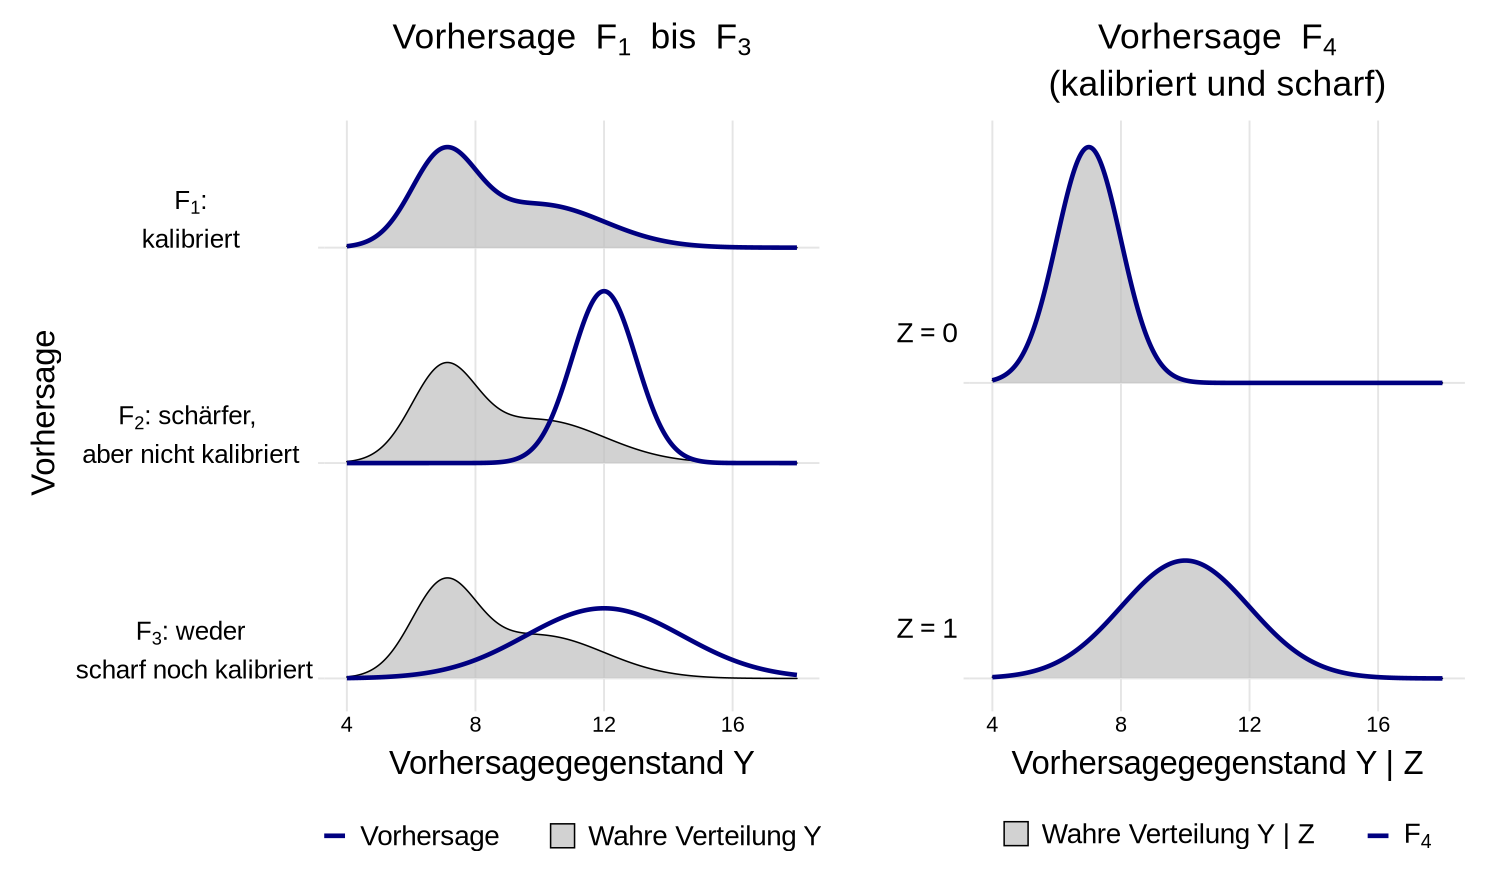
\includegraphics[width=\linewidth]{figs/cal_sharp_visu_Rplot.png}
    \caption{ Verteilung der Vorhersagen im Vergleich zur wahren Verteilung aus Beispiel \ref{bsp:cal_sharp}.
    }
    \label{fig:cal_sharp_visu}
\end{figure}{}

Zur quantitativen Gesamtbewertung der Vorhersagegüte werden schließlich Scoring-Rules oder Scores verwendet \parencite{gneitingMakingPoint2011}. Dabei handelt es sich um Funktionen, die einer probabilistischen Vorhersage anhand von Verifikationsdaten einen numerischen Wert zuordnen. Auf diese Weise lassen sich unterschiedliche Vorhersagen einfach vergleichen; ein besserer Score entspricht einer höheren Vorhersagegüte. Zudem lassen sich einige Scores in Komponenten zerlegen, die wiederum Kalibrierung und Schärfe getrennt widerspiegeln, wodurch Stärken und Schwächen von Vorhersagen deutlich werden können \parencite{arnold2024decompositions}.




\chapter{Klassische Kalibrierungskonzepte}\label{chap:classic_calibration}
In diesem Kapitel widmen wir uns dem ersten wichtigen Kriterium zur Evaluation probabilistischer Vorhersagen: der Kalibrierung. Hierzu führen wir drei grundlegenden Begriffe der Kalibrierung ein. Die formale Definition des Vorhersageraums aus Definition \ref{def::room} dient dabei als Rahmen, innerhalb dessen wir diese Begriffe definieren. Im Mittelpunkt steht insbesondere die Frage, wie sich die stochastische Konzeption von Kalibrierung empirisch übersetzten lässt. Schließlich werden dazu Reliabilitätsdiagramme vorgestellt, die eine visuelle, empirische Beurteilung der Kalibrierung ermöglichen.

\section{Auto-Kalibrierung} \label{sec:auto_cal}
Im Folgenden beschreiben wir mit $\mathcal{L}$ eine bedingte oder unbedingte Wahrscheinlichkeitsverteilung identifiziert durch ihre Verteilungsfunktion. Wir schreiben \[\mathcal{L}(Y \mid F)\coloneqq\mathcal{L}(Y \mid \sigma(F))\] für die bedingte Verteilung von $Y$ gegeben der, durch die Vorhersage $F$ erzeugten $\sigma$-Algebra.

\begin{defi}[Auto-Kalibrierung \parencite{gneiting2023regression}]
\label{def::auto}
Eine Vorhersage $F$ heißt \emph{auto-kalibriert} bzgl. $Y$, wenn sie, gegeben der von ihr verwendeten Information, ideal ist. D.h.
\begin{equation}
\LW(Y \mid F) = F \qquad \text{fast sicher}
\end{equation}
oder äquivalent
\begin{equation}\label{eq:auto}
\forall y \in \R: \;  \PW(Y \le y \mid F) = F(y) \qquad \text{fast sicher}.
\end{equation}{}
\end{defi}

Eine auto-kalibrierte Vorhersage reproduziert somit exakt die Struktur des Vorhersagegegenstands, gegeben der Information, die die Vorhersage nutzt; sie nutzt ihre Information optimal. Bei der Überprüfung von Vorhersagen hinsichtlich ihrer Kalibrierung ist Auto-Kalibrierung daher das eigentliche Ziel.

\begin{bsp}[Ideale und marginale Vorhersage sind auto-kalibriert \texorpdfstring{\parencite[Example 2.4]{gneitingCombining2013,Gneiting2007}})]  \label{bsp:auto_kal}
Sei $Y$ ein Vorhersagegegenstand mit 
\[
Y = \mu + \varepsilon \quad \text{wobei} \quad \mu,\; \varepsilon \sim \N(0,1), \quad \mu \indep \varepsilon.
\]
Dabei kann $\mu$ als zufälliger latenter Zustand (z.B. letzter Zustand der Atmosphäre) und $\varepsilon$ als unabhängiges Rauschen interpretiert werden. Wir betrachten jetzt zwei probabilistische Vorhersagen.
\begin{itemize}
    \item Sei $F_1 \coloneqq \N(\mu,1)$. Wir nennen $F_1$ die \emph{ideale Vorhersage}, weil sie den Zustand $\mu$ kennt und optimal verwendet. Daraus ergibt sich die zugehörige Information $\sigma(F_1)=\sigma(\mu)$.
    \item Sei $F_2 \coloneqq \N(0,2)$ die zweite Vorhersage. Wir bezeichnen sie als \emph{marginale Vorhersage}. Sie ist konstant und verwendet keine zusätzliche Information. Daher ist die zugehörige Informationsmenge die triviale $\sigma$-Algebra,  $\sigma(F_2)=\{\emptyset, \Omega\}$.
    \item Für die bedingten Vorhersagen erhalten wir
        \begin{align*}
            \LW(Y \mid F_1)&=\LW(Y \mid \mu)=\N(\mu,1), \\
            \LW(Y \mid F_2)&=\LW(Y)=\N(0,2).
        \end{align*}
    Somit sind sowohl $F_1$ als auch $F_2$ jeweils auto-kalibriert.
\end{itemize}
Dieses Beispiel verdeutlicht außerdem, dass Auto-Kalibrierung allein nicht ausreicht, um die Qualität einer Vorhersage zu bewerten. Obwohl sowohl $F_1$ als auch $F_2$ auto-kalibriert sind, liefert $F_1$ aufgrund der zusätzlichen Information über $\mu$ die deutlich präzisere (schärfere) und damit bessere Vorhersage. 
\end{bsp}{}


Für kontinuierliche Größen wie Temperatur gibt es im Allgemeinen empirisch keine gute Möglichkeit, Auto-Kalibrierung direkt zu überprüfen \parencite{gneitingCombining2013}, weshalb Auto-Kalibrierung eher ein theoretisches Ideal ist. Der Grund hierfür ist, dass sich die Vorhersageverteilungen in der Praxis häufig von Beobachtung zu Beobachtung unterscheiden, sodass die bedingte Verteilung von $Y$ gegeben $F$ empirisch nicht zuverlässig, selbst mit vielen Daten, geschätzt werden kann. Daher greift man auf andere, schwächere Konzepte der Kalibrierung zurück. Im Folgenden führen wir hierzu die probabilistische und die marginale Kalibrierung ein.

%independence erläutern
%Vielleicht noch isotone Kalibrierung erwähen


\section{Marginale Kalibrierung}\label{sec:marg_cal}
\subsection{Definition}
Eine erste einfache Möglichkeit zur Überprüfung von Kalibrierung besteht darin zu untersuchen, ob Vorhersagegegenstand und Vorhersage im Mittel (d.h. über alle Vorhersagesituationen hinweg) dieselbe Verteilung besitzen. Diese Form der Kalibrierung bezeichnen wir als \emph{marginale Kalibrierung}.

\begin{defi}[Marginale Kalibrierung \parencite{gneiting2023regression}]
Die Vorhersage $F$ heißt \emph{marginal kalibriert}  bzgl. $Y$, falls
\[
\forall y \in \R: \; \; \PW(Y \leq y) = \E_\PW \big[F(y)\big],
\]
wobei der Erwartungswert bezüglich der zufälligen Vorhersage $F$ gebildet wird.
\end{defi}{}

%Marginale Kalibrierung bedeutet, dass die marginale Verteilung der Vorhersagen mit der marginalen Verteilung des Vorhersagegegenstands übereinstimmt.


\subsection{Empirische Überprüfung}
Empirisch betrachten wir nun Vorhersage-Beobachtungspaare der Form \eqref{eq:stich}. Zunächst definieren wir empirische Versionen der marginalen Vorhersageverteilung und der marginalen Verteilungsfunktion des Vorhersagegegenstands.

%gneiting resin 2023
\begin{defi}[Empirisch marginale Vorhersageverteilung und empirisch marginale Verteilung des Vorhersagegegenstandes \parencite{gneiting2023regression}]
Seien Vorhersage-Beobachtungspaare der Form \eqref{eq:stich} gegeben und $y \in \R$. Dann lautet die empirische marginale Vorhersage oder mittlere Vorhersage
\begin{equation} \label{eq:F_mg}
   \hat{F}_{mg}(y)\coloneqq\frac{1}{n}\sum_{i=1}^{n}F_i(y). 
\end{equation}
Die empirisch marginale Verteilung des Vorhersagegegenstandes schreiben wir als
\begin{equation} \label{eq:Y_mg}
\widehat{\PW}(Y \leq y)\coloneqq\frac{1}{n}\sum_{i=1}^{n}\mathds{1}\{y_i\leq y\}.
\end{equation}

\end{defi}

Für Temperaturvorhersagen bedeutet dies, dass die über die betrachteten Vorhersagezeitpunkte oder Orte aggregierte Verteilung der vorhergesagten Temperaturen mit der entsprechenden marginalen Verteilung der tatsächlich beobachteten Temperaturen übereinstimmt. Die Vorhersage erfasst damit das zugrunde liegende Klimaniveau \parencite{Gneiting2007}.

Marginale Kalibrierung können wir jetzt visuell überprüfen, indem wir die mittlere Vorhersage gegen die empirische marginale Verteilungsfunktion des Vorhersagegegenstands abbilden. Wir nennen diese Darstellung das \emph{marginale Reliabilitätsdiagramm} \parencite[B.3]{gneiting2023regression}. Liegen die Werte annähernd auf der Diagonalen, ist die marginale Kalibrierung erfüllt. Eine $S$-förmige Abweichung deutet auf eine überdispersive, während eine inverse $S$-Form auf eine unterdispersive marginale Vorhersage hinweist. Zusätzlich weist eine systematische Verschiebung der Kurve über oder unter der Diagonalen auf einen Bias in der Vorhersage hin. Das folgende Beispiel illustriert die Interpretation des Diagramms für  nicht marginal kalibrierte Vorhersagen.

% überdispersive Vorhersage mit negativem Bias, $F = \N(3,50)$; überdispersive Vorhersage mit positivem Bias, $F = \N(7,50)$.

\begin{bsp}[Interpretation des marginalen Reliabilitätsdiagramms] \label{bsp:marg_cal}
Zur Veranschaulichung der Interpretation marginaler Reliabilitätsdiagramme betrachten wir eine Zufallsvariable
\[
Y \sim \N(5,25).
\]
Abbildung \ref{fig:marg_cal} zeigt die marginalen Reliabilitätsdiagramme acht verschiedener statischer probabilistischer Vorhersagen mit prototypischen Fehlern. Hierzu wurden $500$ unabhängige Beobachtungen von $Y$ simuliert und mit den statischen Vorhersagen zu Vorhersage-Beobachtungspaaren zusammengeführt. Dadurch lassen sich verschiedene Formen der Abweichungen von marginalen Kalibrierung veranschaulichen. Wir betrachten folgende Vorhersagen:
\begin{itemize}
\item[(a)] eine unterdispersive Vorhersage $F=\N(5,8)$, bei der die vorhergesagte Varianz kleiner als die tatsächliche Varianz von $Y$ ist.

\item[(b)] eine überdispersive Vorhersage $F=\N(5,50)$, bei der die vorhergesagte Varianz größer als die tatsächliche Varianz ist.

\item[(c)] mit $F=\N(3,25)$ liegt der Erwartungswert der Vorhersage unterhalb des tatsächlichen Erwartungswerts. Es liegt daher ein negativer Bias vor.

\item[(d)] mit $F=\N(7,25)$ liegt der Erwartungswert der Vorhersage oberhalb des tatsächlichen Erwartungswerts, sodass ein positiver Bias vorliegt.

\item[(e)] und (f) kombinieren die zu geringe Streuung aus (a) mit dem negativen bzw. positiven Bias aus (c) bzw. (d).

\item[(g)] und (h) kombinieren die zu hohe Streuung aus (b) mit einem negativen bzw. positiven Bias aus (c) bzw. (d).
\end{itemize}
Wie Abbildung \ref{fig:marg_cal} zu entnehmen ist, lassen sich zusätzlich approximativ Konsistenzbänder einzeichnen. Die Bänder dienen dazu, zu beurteilen, ob die beobachteten Abweichungen von der marginalen Kalibrierung noch mit zufallsbedingten Schwankungen vereinbar sind. Diese wurden hier nach der Methode von \textcite{gneiting2023regression} unter Annahme marginaler Kalibrierung über ein Resampling-Verfahren auf Basis von $1000$ Replikationen erstellt. Das Verfahren ist in Appendix \ref{seq:consist_marg} beschrieben.
\end{bsp}

\begin{figure}
    \centering
    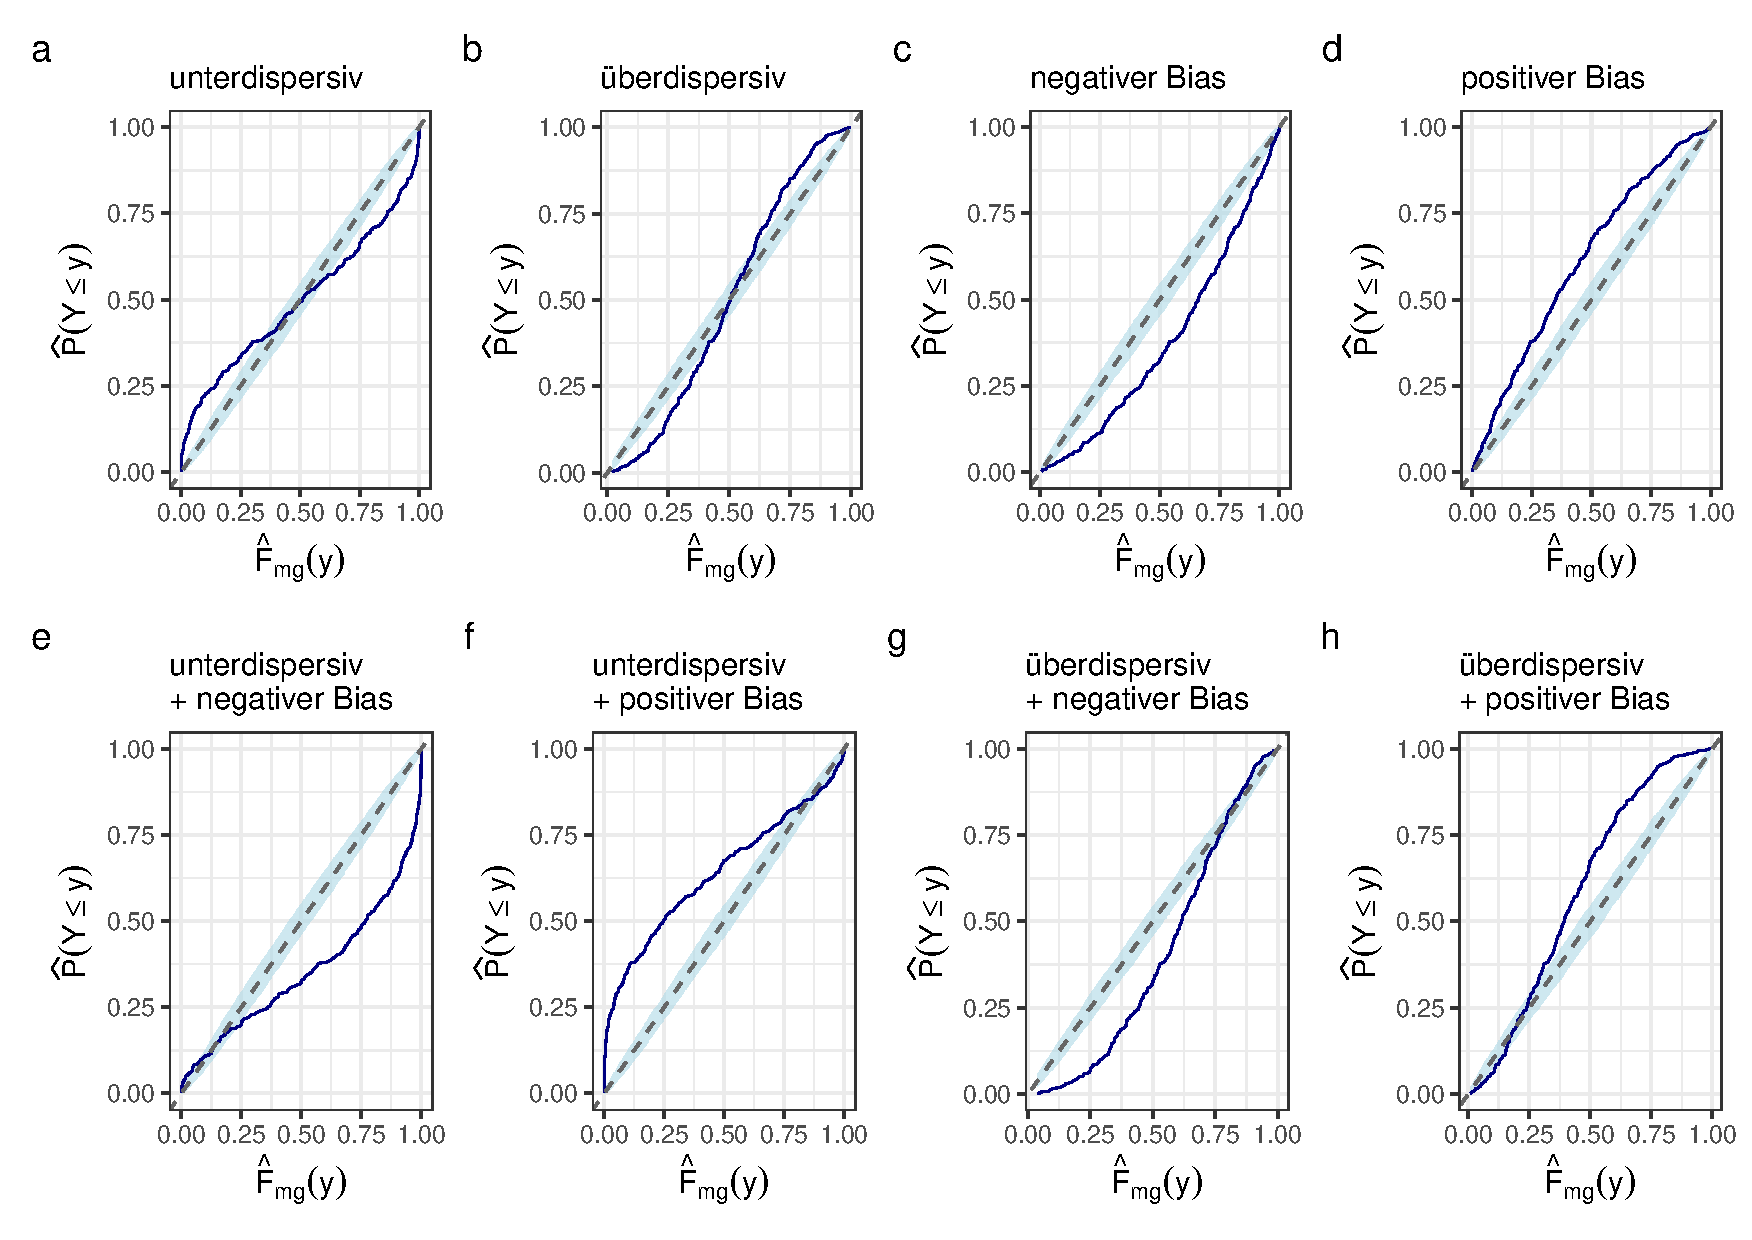
\includegraphics[width=\linewidth]{figs/marg_theo_Rplot.pdf}
    \caption{
    Marginale Reliabilitätsdiagramme zum Beispiel \ref{bsp:marg_cal}.
    }
    \label{fig:marg_cal}
\end{figure}{}


\FloatBarrier
\section{Probabilistische Kalibrierung} \label{sec:pit_cal}
\subsection{Definition} \label{sec:def_prob}
Zur Motivation probabilistischer Kalibrierung betrachten wir zunächst eine grundlegende Eigenschaft von Verteilungsfunktionen. Sei
$X \sim G$
eine Zufallsvariable mit stetiger Verteilungsfunktion $G$. 
Setzten wir nun die Zufallsvariable $X$ selbst in ihre Verteilungsfunktion $G$ ein, erhalten wir die transformierte Zufallsvariable
\begin{equation} \label{eq:pit_intro}
    G(X)
\end{equation}
Für eine stetige Verteilungsfunktion ist diese transformierte Zufallsvariable uniform gleichverteilt \parencite[Theorem 2.1.10]{CasellaBerger2002}. Sie wird als \emph{Wahrscheinlichkeitsintegraltransformation} (engl. \emph{probability integral transform}, PIT) bezeichnet \parencite{gneitingCombining2013}.

Wir können diese Eigenschaft nun nutzen, um die Güte einer probabilistischen Vorhersage zu beurteilen. Dafür betrachten wir wieder einen  Vorhersageraum $(F,Y)$. Ist die Vorhersage $F$ tatsächlich eine passende Beschreibung der Verteilung von $Y$, sollte sich $Y$ unter Anwendung der PIT genauso verhalten wie eine Beobachtung aus $F$. Daher Fordern wir: Eine Vorhersage $F$ ist probabilistisch kalibriert, sofern diese PIT-transformierte Zufallsvariable standarduniformverteilt ist. Also
\[
F(Y) \sim \mathcal{U}(0,1).
\]
Zwei Aspekte sind hier zusätzlich zu berücksichtigen. Besitzt die Verteilungsfunktion, in die die Zufallsvariable im Rahmen der PIT eingesetzt wird, Sprungstellen,  gilt die Gleichverteilung der PIT im Allgemeinen nicht, selbst wenn die Zufallsvariable tatsächlich dieser Verteilung folgt. Wir verallgemeinern daher die PIT auf beliebige Zufallsvariablen, indem wir eine randomisierte Version der Transformation betrachten \parencite{ferguson1967}. Hierzu erweitern wir den Vorhersageraum aus Definition \ref{def::room} um eine von $F$ und $Y$ unabhängige Zufallsvariable $U\sim\mathcal{U}(0,1)$ und betrachten Tupel der Form
\[
(F,Y,U).
\]
Der zweite Aspekt ist, dass im Vorhersageraumsetting die Vorhersage $F$ im Gegensatz zu $G$ in \eqref{eq:pit_intro} nicht fixiert, sondern selbst eine Zufallsgröße ist. Damit können wir nun die randomisierte PIT im Vorhersageraum definieren.


\begin{defi}[Wahrscheinlichkeitsintegral\-transfor\-ma\-tion, PIT \parencite{gneiting2023regression}]
Die Zufallsvariable $Z_F$ nennen wir Wahrscheinlichkeitsintegraltransformation (PIT) falls
\begin{equation}\label{eq:PIT}
Z_F=F(Y^-)+U(F(Y)-F(Y^-)),
\end{equation}{}wobei $F(y^-) := \lim_{x \rightarrow y^-} F(x)$ den linksseitigen Grenzwert von $F$ bezeichnet. Ist $F$ stetig, so vereinfacht sich das zu
\[
Z_F = F(Y).
\]
\end{defi}{}

\begin{defi}[Probabilistische Kalibrierung \parencite{gneiting2023regression}]
Die Vorhersage $F$ heißt \emph{probabilistisch kalibriert} bzgl. $Y$, falls
\begin{equation}\label{eq:PK1}
    Z_F \sim \mathcal{U}(0, 1) 
\end{equation}{}
oder äquivalent
\begin{equation}\label{eq:PK2}
\forall \alpha \in (0,1): \PW\big(Z_F \leq \alpha \big) = \alpha
\end{equation}{}
gilt.
\end{defi}{}

\subsection{Empirische Überprüfung}
Empirisch betrachten wir nun wieder Beobachtungen der Form \eqref{eq:stich}. Zunächst definieren wir empirische Versionen der PIT-Zufallsvariable und ihre Verteilungsfunktion.

\begin{defi}[Empirisches PIT und empirische PIT Verteilung] Seien $u_1,\dotsc,u_n$ unabhängige Realisierungen von $U$.
Die empirischen PIT-Werte erhalten wir, indem wir \eqref{eq:PIT} auf Ebene der Tupel $(F_i,y_i,u_i)$ anwenden. Es gilt
    \[
        z_i \coloneqq F_i(y_i^-) + u_i \cdot \bigl(F_i(y_i) - F_i(y_i^-)\bigr), \quad i = 1,\dots,n.
    \]
    Sind alle $F_i$ stetig, verwenden wir stattdessen
    \[
        z_i \coloneqq F_i(y_i).
    \]
    Die empirische PIT Verteilung lautet dann für $\alpha \in (0,1)$
    \begin{equation} \label{eq:emp_pit_dist}
        \widehat{\PW}(Z_F \leq \alpha) = \frac{1}{n}\sum_{i=1}^{n}\mathds{1}\{z_i\leq \alpha\}.
    \end{equation}
\end{defi}{}

Visuell können wir probabilistische Kalibrierung auf zwei verschiedene Arten überprüfen. Die erste (klassische und verbreitete) Variante ist das \emph{PIT-Histogramm} \parencite{gneiting2014probabilistic,gneitingCombining2013}. Hier überprüfen wir probabilistische Kalibrierung in der Darstellung gemäß \eqref{eq:PK1}, indem wir die empirischen PIT Werte in Form eines auf Dichte normierten Histogramms darstellen. Probabilistische Kalibrierung ist erfüllt, sofern das PIT-Histogramm annähernd flach ist. U-förmige Histogramme weisen auf unterdisperse Vorhersageverteilungen hin, während glockenförmige Histogramme auf überdisperse Vorhersageverteilungen deuten.

Die zweite Variante entspricht der Überprüfung von \eqref{eq:PK2}. Hierbei stellen wir die empirische PIT Verteilungsfunktion  \eqref{eq:emp_pit_dist} graphisch dar. Wir nennen diese Variante das \emph{PIT-Reliabilitätsdiagramm}. Der Vorteil gegenüber dem PIT-Histogramm besteht darin, dass die Darstellung nicht von der Wahl der Bins abhängt, weil unterschiedliche Binnings zu variierenden visuellen Eindrücken führen und dadurch Kalibrierungsfehler entweder verdecken oder scheinbar verstärken können \parencite{gneiting2023regression}. Das PIT-Reliabilitätsdiagramm interpretieren wir analog zum marginalen Reliabilitätsdiagramm. Abbildung \ref{fig:pit_cal} illustriert schematische Beispiele zur Einordnung des Reliabilitätsdiagramms und Histogramms.


\begin{bsp}[Interpretation des PIT-Reliabilitätsdiagramms und des PIT-Histogramms] \label{bsp:pit_cal}
Zur Veranschaulichung der Interpretation von PIT-Reliabilitäts\-diagramm und PIT-Histo\-gramm betrachten wir den Vorhersage\-gegenstand und die Vorhersagen aus Beispiel \ref{bsp:marg_cal}. In Abbildung \ref{fig:pit_cal} sind die zu den Vorhersagen korrespondierenden PIT-Reliabilitätsdiagramme und PIT-Histogramme dargestellt. Die PIT-Histogramme wurden jeweils mit $20$ Bins erstellt. Die folgenden Vorhersagen sind den jeweiligen Plots zugeordnet:
%checken, das das wirklich richtig zugeordnet ist
\begin{itemize}
\item[(a-b)] die unterdispersive Vorhersage.

\item[(c-d)] die überdispersive Vorhersage.

\item[(e-f)] die Vorhersage mit negativem Bias.

\item[(g-h)] die Vorhersage mit positivem Bias.

\item[(i-j)] und (m-n) unterdispersive Vorhersagen mit negativem beziehungsweise positivem Bias.

\item[(k-l)] und (o-p) uberdispersive Vorhersagen mit negativem beziehungsweise positivem Bias.

\end{itemize}
Dem Reliabilitätsdiagramm können wir wieder ein Konsistenzband anfügen. Das hier verwendete Verfahren ist in Appendix \ref{seq:consist_pit} beschrieben.
\end{bsp}

\begin{figure}
    \centering
    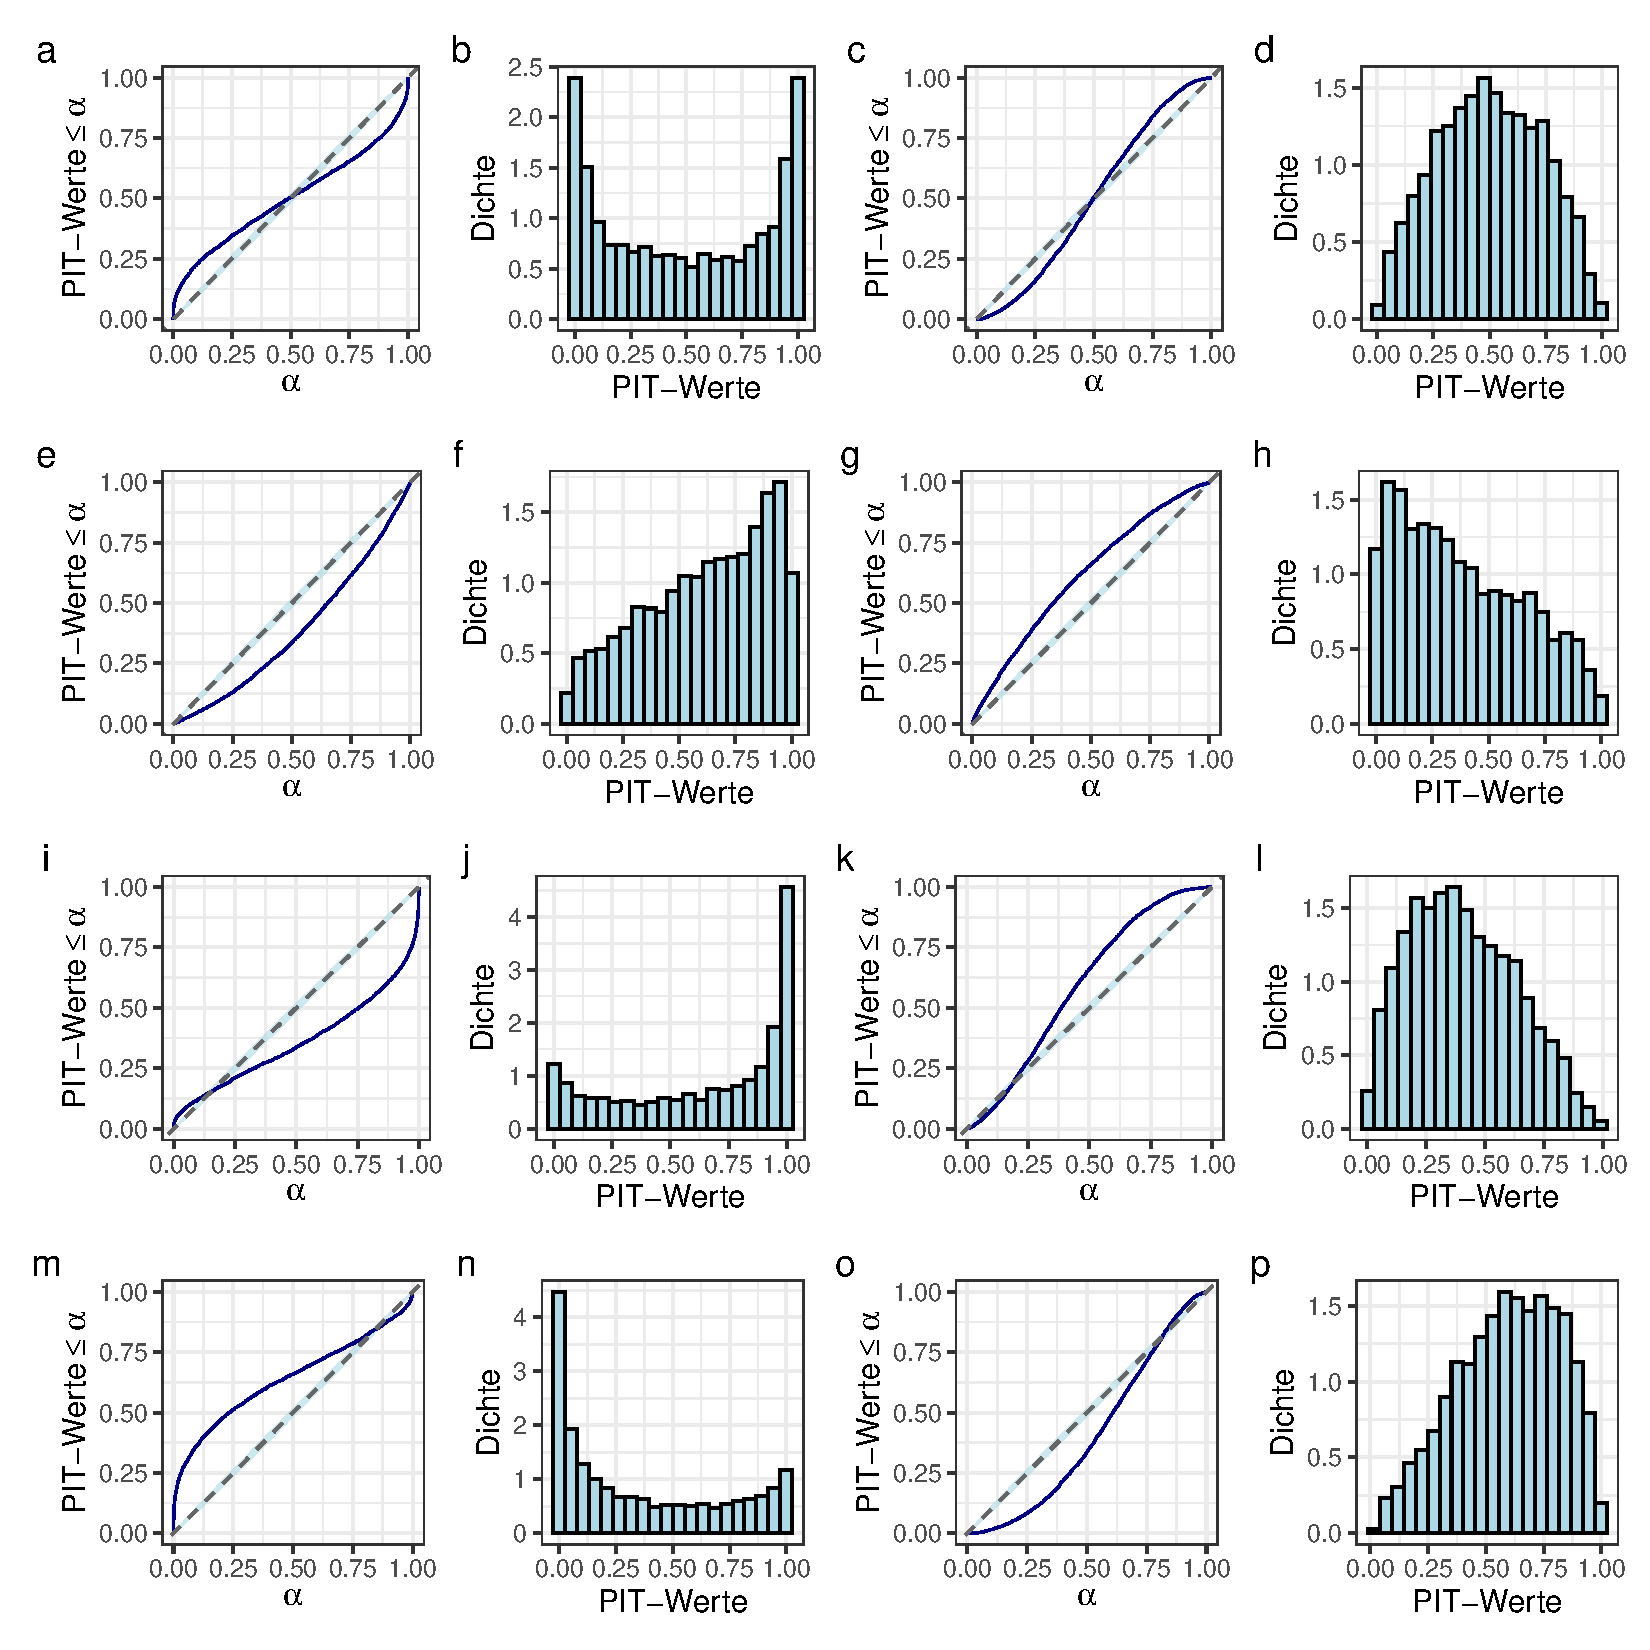
\includegraphics[width=\linewidth]{figs/pit_Rplot.pdf}
    \caption{
    Abbildung zum Beispiel \ref{bsp:pit_cal} zur Interpretation des PIT-Reliabi\-litätsdiagramms und PIT-Histogramms.
    }
    \label{fig:pit_cal}
\end{figure}{}


Der im Reliabitlitäsdiagramm gemachte Vergleich von $\widehat{\PW}(Z_F \leq \alpha)$ mit $\alpha$ ermöglicht zudem eine anschauliche Interpretation über die verschiedenen Vorhersagesituationen hinweg. Liegt beispielsweise für $\alpha=0.75$ die empirische PIT Verteilung bei \mbox{$\widehat{\PW}(Z_F\leq 0.75)=0.9$}, so liegen etwa 90\% der beobachteten Realisierungen unterhalb des jeweils vorhergesagten 75\%-Quantilniveaus. Dies deutet darauf hin, dass das 75\%-Quantil über die betrachtete Stichprobe hinweg überschätzt wird. Liegt die empirische PIT Verteilung dagegen bei $0.6$, deutet dies entsprechend auf ein unterschätztes 75\%-Quantil hin. Für das Diagramm bedeutet dies, dass Werte oberhalb der Diagonalen darauf hindeuten, dass die entsprechenden Quantile über die betrachtete Stichprobe hinweg überschätzt werden, Werte unterhalb der Diagonalen deuten tendenziell auf unterschätzte Quantile. Damit lässt sich bereits erkennen, dass die probabilistische Kalibrierung eng mit der (unbedingten) Quantilkalibrierung zusammenhängt, auf die wir im Folgenden Kapitel genauer eingehen.


\chapter{Quantilkalibrierung} \label{chap:quant_cal}
Im vorherigen Kapitel haben wir uns mit klassischen Kalibrierungsbegriffen befasst. Eine alternative Perspektive ergibt sich, wenn wir Kalibrierung auf Basis statistischer Funktionale betrachten, insbesondere zur Untersuchung bedingter Kalibrierung. Stellvertretend betrachten wir hierfür die Quantilkalibrierung, die im Folgenden detailliert vorgestellt wird.

In Abschnitt \ref{seq:T_cal} stellen wir die Grundidee der Kalibrierung auf statistischen Funktionalen vor. Anschließend betrachten wir Quantilkalibrieung in Abschnitt \ref{seq:Quantcal}. Dort führen wir zunächst den Begriff der unbedingten und bedingten $\alpha$-Quantilkalibrierung ein, bevor wir uns mit der empirischen Überprüfung von Quantilkalilbrierung in beschäftigen. Für die Untersuchung der bedingten Quantilkalibrierung erläutern wir dabei den CORP-Ansatz von \textcite{gneiting2023regression}.

\section{Kalibrierung auf statistischen Funktionalen} \label{seq:T_cal}
Bei den bisher eingeführten Kalibrierungsbegriffen haben wir jeweils die gesamte Verteilung des Vorhersagegegenstands sowie der Vorhersage betrachtet. Stattdessen kann Kalibrierung auch anhand einzelner Charakteristika einer probabilistischen Vorhersage untersucht werden, etwa des Erwartungswerts, auf Grundlage von Schwellenwerten oder Quantilen \parencite{gneiting2023regression, jordanOptimalSolutions2022}.

Das hat mehrere Vorteile. Erstens sind solche Betrachtungen oft einfacher und leichter zu interpretieren. Beispielsweise bedeutet die Kalibrierung des Erwartungswertes, dass der Erwartungswert der Vorhersage und Erwartungswert des Vorhersagegegenstands übereinstimmen. Zweitens liegt das Interesse in vielen Anwendungen nicht auf der voll\-ständigen Vorhersageverteilung, sondern nur auf bestimmten Aspekten der Verteilungen, etwa darauf, ob das 25\%- oder 75\%-Quantil korrekt getroffen wird. Drittens ermöglicht dieser Zugang eine natürliche Formulierung bedingter Kalibrierung. Anstatt wie bei der Auto-Kalibrierung auf die gesamte Vorhersage zu konditionieren, wird lediglich auf das vorhergesagte statistische Funktional bedingt. Im Fall des Erwartungswerts bedeutete es, dass der Erwartungswert des Vorhersagegegenstands bedingt auf den vorhergesagten Erwartungswert diesem entspricht. Anschaulich entspricht das der Situation, dass alle Tage mit einer vorhergesagten Durchschnittstemperatur von $20\C$ im Mittel auch tatsächlich eine Temperatur von $20\C$ aufweisen.

Gerade der letzte Aspekt ist für die Überprüfung von Kalibrierung bedeutend, denn marginale und probabilistische Kalibrierung sind unbedingt. Eine ausschließlich auf solchen unbedingten Kalibrierungsbegriffen basierende Evaluation gilt jedoch zunehmend als unzureichend  \parencite{gneiting2023regression}.

Wenn wir nur einzelne Funktionale betrachten, entspricht das der Überprüfung von Punktvorhersagen. Das erlaubt noch keine umfassende Aussage über die gesamte probabilistische Vorhersage. Deshalb betrachten wir einzelne Funktionale nicht allein, sondern Klassen ähnlicher Funktionale, etwa eine Menge an Quantilen bzw. Schwellenwerten, gemeinsam. Dadurch lassen sich Rückschlüsse über ganze Vorhersageverteilungen ziehen.

Im Rahmen der vorliegenden Arbeit konzentrieren wir uns auf die Quantilkalibrierung. Gegenüber der Schwellenwertkalibrierung besitzt sie den Vorteil, unabhängig von der Einheit des Vorhersagegegenstands zu sein \parencite{bentzienDecomposition2014}. Allerdings sind Quantile im Allgemeinen nicht notwendig reellwertig, sondern können mengenwertig auftreten.  Im Folgenden wollen wir jedoch mit reellen Werten arbeiten. Dazu müssen wir die Definition von Quantilkalibrierung entsprechend einschränken.


\section{Quantilkalibrierung} \label{seq:Quantcal}
\subsection{Definiton}
Quantile können mengenwertig sein. Das kann genau dann eintreten, wenn die Verteilungsfunktion nicht streng monoton wächst, sondern auf einem Intervall flach ist oder Sprünge besitzt. Daher unterscheiden wir zwischen unterem und oberem $\alpha$-Quantil \parencite{gneiting2023model}.

\begin{defi}[Unteres und oberes $\alpha$-Quantil  \parencite{gneiting2023model}]
Sei $\alpha \in (0,1)$. Für eine Verteilungsfunktion $F$ definieren wir das untere $\alpha$-Quantil als
\begin{equation}\label{eq:lowerquantile}
    q^-_\alpha(F)
    \coloneqq
    \sup \{ x \in \R : F(x) < \alpha \}
    =
    \inf \{ x \in \R : F(x) \ge \alpha \},
    \end{equation}
    sowie das obere $\alpha$-Quantil als
    \begin{equation}\label{eq:upperquantile}
    q^+_\alpha(F)
    \coloneqq
    \inf \{ x \in \R : F(x) > \alpha \}.
\end{equation}
\noindent
\begin{itemize}
    \item Für das untere Quantil $q^-_\alpha(Y)$ schreiben wir im Folgenden einfach nur  $q_\alpha(Y)$.
    \item Ein gültiges $\alpha$-Quantil von $F$ ist dann ein beliebiges Element aus der Menge 
    \[
    \left[q_\alpha(F),q^+_\alpha(F)\right]
    \].
\end{itemize}
\end{defi}
\noindent
Analog schreiben wir für den Vorhersagegegenstand $Y$ \begin{align*}
    q_\alpha(Y) &\coloneqq  q_\alpha(\LW(Y)) = \inf \{ x \in \R : \PW(Y \le x) \ge \alpha \},\\
    q^+_\alpha(Y)&\coloneqq q^+_\alpha(\LW(Y)) = \inf \{ x \in \R : \PW(Y \le x) > \alpha \}.
\end{align*}
Schließlich bezeichnen wir mit $\hat q_\alpha(\cdot)$ den empirischen Schätzer des unteren $\alpha$-Quantils $q_\alpha(\cdot)$. Zu dessen Berechnung verwenden wir in der vorliegenden Arbeit Definition 1 aus \textcite{hyndman1996sample}, nach der das empirische $\alpha$-Quantil durch die verallgemeinerte Inverse der empirischen Verteilungsfunktion gegeben ist.
 
Als nächstes führen wir die Quantilkalibrierung ein. In der Literatur finden sich jedoch leicht verschiedene, eng verwandte Definitionen dieser, die wir im Folgenden auflisten. Wir unterscheiden zwischen einer unbedingten Variante, die keine weitere Vorhersageinformation nutzt und einer bedingten. 

\begin{defi}[$\alpha$-Quantilkalibrierung]
Eine Vorhersage $F$ heißt \emph{unbedingt $\alpha$-quantil\-kalibriert} für ein $\alpha  \in (0,1)$  bzgl. $Y$   falls
\begin{equation}\label{eq:uncond_pm_quant_cal}
    \PW(Y \leq q_\alpha(F)) \ge \alpha \quad \text{und} \quad  \PW(Y < q^+_\alpha(F)) \leq \alpha
\end{equation}
gilt. Diese Darstellung entspricht Gleichung (10) aus \textcite{gneiting2023regression}. 

Die \emph{unbedingte $\alpha$-Quantilkalibrierung} überprüft also, ob die vorhergesagten $\alpha$-Quantile $q^\pm_{\alpha}(F)$ die korrekten marginalen Überdeckungswahrscheinlichkeiten aufweisen. Im Rahmen des Vorhersageraums ist die Vorhersage $F$ als Markovkern zufallsabhängig. Daher sind auch die induzierten Quantile $q^\pm_{\alpha}(F)$ im Allgemeinen wieder Zufallsvariablen. Die unbedingte $\alpha$-Quantilkalibrierung ist daher eine marginale Eigenschaft der gemeinsamen Verteilung $(F,Y)$. Wir betrachten nun eine leicht abgeschwächte Variante, die ausschließlich auf dem unteren vorhergesagten Quantil basiert:
\begin{equation}\label{eq:unb_quantcal_lower}
    \quad \PW(Y \leq q_\alpha(F)) \ge \alpha \quad \text{und} \quad  \PW(Y < q_\alpha(F)) \leq \alpha.
\end{equation}{}
Diese Einschränkung stellt in der Praxis keine wesentliche Einbuße dar, weil die Quantile in den meisten Fällen eindeutig sind \parencite{arnold2025isotonic}. Sie hat jedoch den Vorteil, dass wir immer eindeutige Werte für die vorhergesagten $\alpha$-Quantile verwenden.

Für \emph{bedingte $\alpha$-Quantilkalibrierung}, bedingen wir \eqref{eq:unb_quantcal_lower} auf das vorhergesagte $\alpha$-Quantil. Die Vorhersage $F$ heißt bedingt $\alpha$-quantilkalibriert für ein $\alpha \in (0,1)$ bzgl. $Y$ falls
\begin{equation}\label{eq:cond_quantcal_lower}
    \quad \PW(Y \leq q_\alpha(F) \mid q_\alpha(F)) \ge \alpha \quad \text{und} \quad  \PW(Y < q_\alpha(F) \mid q_\alpha(F)) \leq \alpha
\end{equation}{}
gilt.
Diese Definition entspricht Gleichung (2) aus \textcite{gneiting2023model}.
Im Gegensatz zur unbedingten Quantilkalibrierung wird hier nicht nur die marginale Überdeckungs\-wahrscheinlichkeit betrachtet. Stattdessen prüfen wir, ob die Vorhersagen auch bedingt auf das jeweils vorhergesagte Quantil korrekt kalibriert sind.

Die Bedingung in \eqref{eq:cond_quantcal_lower} kontrolliert weiterhin Überdeckungswahrscheinlichkeiten. Eine leicht stärkere Forderung besteht darin zu verlangen, dass das vorhergesagte Quantil exakt dem entsprechenden Quantil der bedingten Verteilung von $Y$ entspricht. Dies führt zur folgenden Definition gemäß Gleichung (10) aus \textcite{arnold2025isotonic}. Sie lautet: Die Vorhersage $F$ heißt \emph{bedingt $\alpha$-quantilkalibriert} für ein $\alpha \in (0,1)$ bzgl. $Y$ falls
\begin{equation}\label{eq:cond_alpha_quant_cal}
\quad q_\alpha\left(Y \mid q_\alpha(F)\right) = q_\alpha(F)\quad \text{fast sicher}
\end{equation}
gilt. Es besteht Äquivalenz zu \eqref{eq:cond_quantcal_lower}, sofern das bedingte $\alpha$-Quantil von $Y$ eindeutig ist. 

Diese letzte Darstellung führen wir ein, weil sie in direkter Nähe zur empirischen Überprüfung der bedingten $\alpha$-Quantilkalibrierung steht, die wir mithilfe eines Reliabilitätsdiagramms umsetzen werden. Zudem bietet sie eine unmittelbare intuitive Interpretation: Immer wenn ein $\alpha$-Quantil von beispielsweise $10\C$ vorhergesagt wird, soll auch das tatsächliche $\alpha$-Quantil der bedingten Verteilung bei $10\C$ liegen.
\end{defi}{}

Aktuell betrachten wir nur ein einziges $\alpha$-Quantil. Das entspricht der Überprüfung einer Punktvorhersage und lässt somit noch keinen guten Rückschluss auf die Güte einer kompletten Vorhersageverteilung zu. Betrachten wir theoretisch jedoch alle $\alpha$-Quantile zusammen, können wir die Kalibrierung der gesamten Vorhersage beurteilen. Mit diesem Hintergrund definieren wir  \emph{(bedingte) Quantilkalibrierung}.
\begin{defi}[(bedingte) Quantilkalibrierung] \label{def:all_quantcal}
Eine Vorhersage $F$ heiß quantilkalibriert bzgl. $Y$ falls
\[
\forall \alpha \in (0,1): \quad q_\alpha\left(Y\mid q_\alpha(F)\right) = q_\alpha(F)\quad \text{fast sicher}
\]
gilt.
\end{defi}


\subsection{Empirische Überprüfung}\label{sec:emp_prüf_quantcal}
Zur Überprüfung der Quantilkalibrierung beschränken wir uns zunächst auf ein festes $\alpha \in (0,1)$. Anstatt der gemeinsamen Verteilung von $(F,Y)$ betrachten wir nu das Paar
\begin{equation} \label{eq:qaunt_stich_pop}
 (X,Y) \quad \text{mit} \quad X \coloneqq q_\alpha(F).   
\end{equation}
Entsprechend erhalten wir als Stichprobe Vorhersage-Beobachtungspaare der Gestalt
\begin{equation} \label{eq:qaunt_stich_emp}
    (x_1, y_1), \dotsc, (x_n, y_n) \quad \text{mit} \quad x_i \coloneqq q_\alpha(F_i).
\end{equation}

Zunächst überprüfen wir unbedingte $\alpha$-Quantilkalibrierung gemäß \eqref{eq:unb_quantcal_lower}. Sie lässt sich anhand \emph{empirischer Überdeckungswahrscheinlichkeiten} überprüfen \parencite{gneiting2023model}. Wir verlangen 
\begin{equation}\label{eq:coverage} 
\widehat{\PW}(Y\leq q_{\alpha}(F))=\frac{1}{n}\sum_{i=1}^{n}\mathds{1}\big\{y_i\leq x_i\big\}\ge \alpha
\end{equation}
sowie 
\begin{equation}\label{eq:coverage_low} 
\widehat{\PW}(Y < q_{\alpha}(F))=\frac{1}{n}\sum_{i=1}^{n}\mathds{1}\big\{y_i< x_i\big\} \le \alpha.
\end{equation}
Zur Visualisierung der Überdeckungswahrscheinlichkeiten über verschiedene Werte von $\alpha$ eignen sich sogenannte Coverage-Plots \parencite{gneiting2023model}. Auf diese gehen wir hier nicht näher ein, denn die Überprüfung probabilistischer Kalibrierung aus Abschnitt \ref{sec:pit_cal} impliziert bereits unbedingte Quantilkalibrierung für alle $\alpha \in (0,1)$ (siehe Theorem \ref{theo:pK-unbQK}).

Als Nächstes betrachten wir bedingte $\alpha$-Quantilkalibrierung. Dazu führen wir erneut ein \emph{Reliabilitätsdiagramm} ein. Dieses illustriert die bedingten $\alpha$-Quantile des Vorhersagegegenstands in Abhängigkeit vom vorhergesagten $\alpha$-Quantil \parencite{gneiting2023regression,gneiting2023model}
\begin{equation}\label{eq:rediag}
    x \mapsto q_\alpha(Y \mid X = x).
\end{equation}
Daraus ergibt sich das \emph{empirische Reliabilitätsdiagramm} als die Abbildung
\begin{equation}\label{eq:emp_rediag}
    x_i \mapsto \hat q_\alpha(Y \mid X = x_i).
\end{equation} Die zu schätzenden bedingten Quantile
\[
\hat{q}_\alpha(Y \mid X = x_i)
\]
bezeichnen wir dabei als \emph{rekalibrierte Werte}. Die zentrale Herausforderung besteht darin, diese Größen zu schätzen. 

Grundsätzlich besteht unser Vorgehen darin, ähnliche Vorhersagen zu gruppieren und das empirische Quantil der Beobachtungen innerhalb dieser Gruppen (Bins) als Schätzer für die rekalibrierten Werte zu verwenden. Dabei stellt sich jedoch die Frage, wie genau die Bins zu wählen sind.

Eine Möglichkeit ist der CORP-Ansatz von \textcite{gneiting2023regression}, der auf nichtparametrischer monotoner Regression basiert. Diese wird mittels des sogenannten Pool-adjacent-violator (PAV) Algorithmus umgesetzt, der die Daten durch sukzessives Zusammenfassen benachbarter Vorhersage-Beobachtungspaare so anpasst, dass die resultierende Schätzung des Reliabilitätsdiagramms monoton steigend bzgl. der Ordnung der Vorhersagen wird. So entsteht eine stückweise konstante monoton steigende Funktion, deren Abschnitte die Bins darstellen.

Zentrale Voraussetzung des CORP-Ansatzes ist die \emph{Monotonieannahme}. Sie besagt, dass die Ordnung der Vorhersagen die Ordnung der wahren bedingten Quantile widerspiegelt. Übertragen auf die rekalibrierten Werte fordern wir
\begin{equation}\label{eq:isotone_asump}
 x_i < x_j \quad \Rightarrow \quad  \hat q_\alpha(Y \mid X=x_i) \leq \hat q_\alpha(Y \mid X=x_j).   
\end{equation}
Diese Annahme erlaubt systematische Verzerrungen in den Vorhersagen, solange die Rangordnung erhalten bleibt. Verletzungen dieser Struktur werden in der Regel als Rauschen bzw. Artefakte interpretiert, sodass die Annahme plausibel erscheint \parencite{gneiting2023regression}.

Außerdem fordern wir, dass das empirische Reliabilitätsdiagramm wohldefiniert ist. Daher fordern wir für gleiche Vorhersagen gleiche rekalibrierte Werte:
\[
x_i = x_j \quad \Rightarrow \quad \hat q_\alpha(Y \mid X=x_i) = \hat q_\alpha(Y \mid X=x_j).
\]

Zur Konstruktion solcher rekalibrierter Werte müssen die Vorhersage-Beobachtungspaare geeignet geordnet werden. Hierzu sortieren wir zunächst nach den Vorhersagen $x_i$ aufsteigend und brechen Gleichstände durch absteigende Sortierung der Beobachtungen $y_i$ \parencite[vgl.][]{gneiting2023supp}. Dieses Vorgehen definiert die Ordnung
\begin{equation}\label{eq:pav_order}
(x_i,y_i) \preceq (x_j,y_j)
\;\coloneqq\;
\begin{cases}
\text{wahr}, & \text{falls } x_i < x_j,\\[0.3em]
\text{wahr}, & \text{falls } x_i = x_j \text{ und } y_i \ge y_j,\\[0.3em]
\text{falsch}, & \text{sonst}.
\end{cases}
\end{equation}{}

Die so geordnete Folge von Beobachtungs-Vorhersagepaaren unterziehen wir anschließend dem PAV-Algorithmus und erhalten damit rekalibrierte Werte, die die Monotoniebedingung erfüllen. Beispiel \ref{bsp:order_pav_explain} veranschaulicht, weshalb wir diese Ordnung verwenden. Zunächst beschreiben wir jedoch den PAV-Algorithmus für Quantile orientiert an \textcite[Algorithm 1]{gneiting2023regression}. Dazu definieren wir
\[
\hat{x}_i \coloneqq \hat{q}_\alpha(Y \mid X = x_i).
\]
\begin{alg}[PAV-Algorithmus für Quantile] \label{alq:pava}
Seien O.B.d.A $(x_1,y_1) \preceq \dotsc \preceq (x_n,y_n)$, dann erzeugt der PAV-Algorithmus die für das $\alpha$-Quantil rekalibrierten Paare 
        $(x_1,\hat x_1), \dotsc, (x_n,\hat x_n)$  mit  $\hat x_i \le \dotsc \le \hat x_n$, sodass das empirische Reliabilitätsdiagramm wohldefiniert ist.
\begin{enumerate}
    \item Erzeuge für jeden Datenpunkt einen eigenen Bin, $B_{1:1}=\{x_1\}, \dots,B_{n:n}=\{x_n\}$,
    wobei $B_{i:j}=\{x_k \mid i\leq k \leq j \}\,$ gilt.
    \item Initialisiere den Wert für die rekalibrierten Werte jedes Bins mit der korrespondierenden Beobachtung 
    \[
    \hat x_{B_{i:i}}=y_i \quad \text{für } i=1,\dotsc,n.
    \]  
    \item Pooling-Step: Falls in zwei \emph{benachbarten} Bins $B_{k:i}$, $B_{(i+1):m}$ die Monotoniebedingung verletzt ist (d.h. $\hat x_{B_{k:i}} > \hat x_{B_{(i+1):m}}$),
    \begin{itemize}
        \item Poole die beiden Bins zu $B_{k:m}=\{x_k, \dotsc, x_m\}$
        \item Bestimme den rekalibrierten Wert des neuen Bins $B_{k:m}$ als 
        \[
            \hat x_{B_{k:m}}= q_\alpha\left(\frac{1}{\left| B_{k:m} \right|}\sum_{i=k}^m \mathds{1}\{y_i\leq y\}\right),
        \]
        wobei mit der rechten Seite das $\alpha$-Quantil der empirischen Verteilungsfunktion der Beobachtungen $y_k,\dotsc,y_m$ gemeint ist.
    \end{itemize}{}
    \item Wiederhole Schritt 3, bis keine Monotonieverletzungen mehr vorliegen.
    \item Sei $\mathcal{B}$ die verbleibende Menge an Bins. Weise jedem Punkt innerhalb eines Bins denselben rekalibrierten Wert zu:
    \[
    \forall B \in \mathcal{B}: \quad \hat x_i = \hat x_B \quad \text{für alle } x_i \in B.
     \]
    \item Gib die rekalibrierten Paare 
    \[
        (x_1,\hat x_1), \dotsc, (x_n,\hat x_n) \quad \text{mit }  \hat x_1 \le \dotsc \le \hat x_n
    \]
    zurück.
\end{enumerate}
\end{alg}

\begin{bsp}[Begründung der Ordnung für den PAV-Algorithmus] \label{bsp:order_pav_explain}
Wir betrachten den PAV-Algorithmus für das $50\%$-Quantil. Anhand eines Beispiels soll verdeutlicht werden, warum ein Sortieren allein anhand der Vorhersagen scheitert. Wir betrachten die Paare
\[
(1,1), (2,2), (2,3), (2,5),
\]
Diese sind schon anhand der Vorhersagen aufsteigend geordnet  $(1 \le 2 \le 2 \le 2)$. Wenden wir den PAV-Algorithmus in dieser Reihenfolge an, treten nach Schritt $2$ keine Monotonieverletzungen $(1 \le 2 \le 3 \le 5)$ auf, sodass die Zuordnung unverändert bleibt:
\[
(1,1), (2,2), (2,3), (2,5).
\]
Jetzt haben die gleichen Vorhersagen (mit dem Wert $2$) unterschiedliche rekalibrierte Werte. Sortieren wir die Paare hingegen gemäß \eqref{eq:pav_order}, erhalten wir die Reihenfolge
\[
(1,1), (2,5), (2,3), (2,2).
\]
Bei Anwendung des PAV-Algorithmus haben wir nun Monotonieverletzungen und erhalten nach dessen Anwendung
\[
(1,1), (2,3), (2,3), (2,3).
\]
Damit werden allen Beobachtungen mit gleicher Vorhersage auch identische rekalibrierte Werte zugewiesen, wodurch das empirische Reliabilitätsdiagramm als wohldefinierte Funktion interpretierbar ist.\\
\end{bsp}

Schließlich visualisieren wir die Kalibrierung durch das Verbinden der vom PAV-Algorithmus erhaltenen Punkte
\[
(x_1,\hat x_1), \dotsc, (x_n,\hat x_n).
\]
Wir nennen diese Darstellung das \emph{empirisches Reliabilitätsdiagramm} \parencite{gneiting2023regression}.

Eine Vorhersage ist gut kalibriert, wenn die Punkte auf der Diagonalen liegen. Punkte unterhalb der Diagonalen bedeuten, dass die vorhergesagten bedingten Quantile die beobachteten bedingten Quantile überschätzen, während Punkte oberhalb der Diagonalen auf eine Unterschätzung der beobachteten Quantile durch die vorhergesagten Quantile hindeuten. Darüber hinaus weisen größere horizontale Abschnitte auf eine starke Verletzung der Monotonie der Vorhersagen \eqref{eq:isotone_asump} hin und sind ebenfalls ein Zeichen mangelnder Kalibrierung \parencite{gneiting2023regression}, wobei horizontale Abschnitte an den Rändern durch begrenzte Stichprobengröße oder Ausreißer entstehen können. Sie sind daher nicht zwangsläufig ein Hinweis auf eine schlechte Kalibrierung. Das folgende Beispiel verdeutlicht den Nutzen und die Interpretation des Reliabilitätsdiagramms.

\begin{bsp}[Unfokussierte Vorhersage ist unbedingt aber nicht bedingt quantilkalibriert]\label{bsp:quant_cal}
Wir betrachten den Vorhersagegegenstand aus Beispiel \ref{bsp:auto_kal} und dazu die Vorhersage 
\[
F_3=\frac{1}{2}\N(\mu,1)+\frac{1}{2}\N(\mu + \tau,1).
\]
Es handelt sich um eine Mischverteilung, wobei wir $\tau$ gleichwahrscheinlich aus $\tau \in \{-2,2\}$ und unabhängig von $\mu$ wählen. Wir nennen diese Vorhersage unfokussiert, weil sie den Zustand $\mu$ kennt, aber zusätzlich künstliche Unsicherheit durch $\tau$ einführt \parencite[Example 2.2]{gneiting2023regression}.

Es lässt sich zeigen, dass diese Vorhersage unbedingt, jedoch nicht bedingt quantilkalibriert ist.  Wir überprüfen exemplarisch die Kalibrierung für das $50\%$-Quantil. Zunächst simulieren wir $1000$ Ziehungen aus $\tau$, $\mu$ und $Y$. Damit erstellen wir unabhängige Vorhersage-Beobachtungspaare $(x_1,y_1),\dotsc, (x_{1000},y_{1000})$ mit $x_i = q_{0.5}(F_i)$. Um das Quantil der Mischverteilung zu bestimmen, nutzen wir eine numerische Nullstellensuche.

Die unbedingte $50\%$-Quantilkalibrierung erkennen wir daran, dass für die empirische \\ Überdeckungswahrscheinlichkeit
\[
\widehat{\PW}(Y\leq q_{0.5}(F)) = \frac{1}{1000} \sum_{i=1}^{1000}\mathds{1}\big\{y_i\leq q_{0.5}(F_i)\big\} \approx 0.5
\]
gilt.

Für die bedingte Kalibrierung erstellen wir das empirische Reliabilitätsdiagramm Abbildung \ref{fig:quant_cal}). Neben der Reliabilitätskurve haben wir die Vorhersage-Beobachtungspaare als Punktwolke dargestellt, um ein umfassenderes Gesamtbild zu erhalten. Dabei zeigt sich, dass die Beobachtungen vor allem im mittleren Bereich konzentriert sind, während nur wenige extreme Vorhersagen bzw. Beobachtungen vorliegen. Daher ist die Reliabilitätskurve in den Randbereichen mit größerer Unsicherheit behaftet und entsprechend weniger verlässlich. 

Zwischen $-3$ und $-1$ liegen die rekalibrierten Werte oberhalb der Diagonalen und außerhalb des Konsistenzbandes. Dies bedeutet, dass die Vorhersagen die beobachteten Quantile in diesem Bereich unterschätzen. Zwischen $0.5$ und $2$ liegen die rekalibrierten Werte hingegen unterhalb der Diagonalen und ebenfalls außerhalb des Konsistenzbandes, was darauf hindeutet, dass die Vorhersagen die beobachteten Quantile in diesem Bereich überschätzen. Insgesamt zeigt sich somit, dass die Quantile sowohl über- als auch unterschätzt werden. Diese gegenläufigen Kalibrierungsfehler gleichen sich bei der Betrachtung der unbedingten Quantilkalibrierung jedoch weitgehend aus, sodass Vorhersage diese Bedingung erfüllt.

\end{bsp}

\begin{figure}
    \centering
    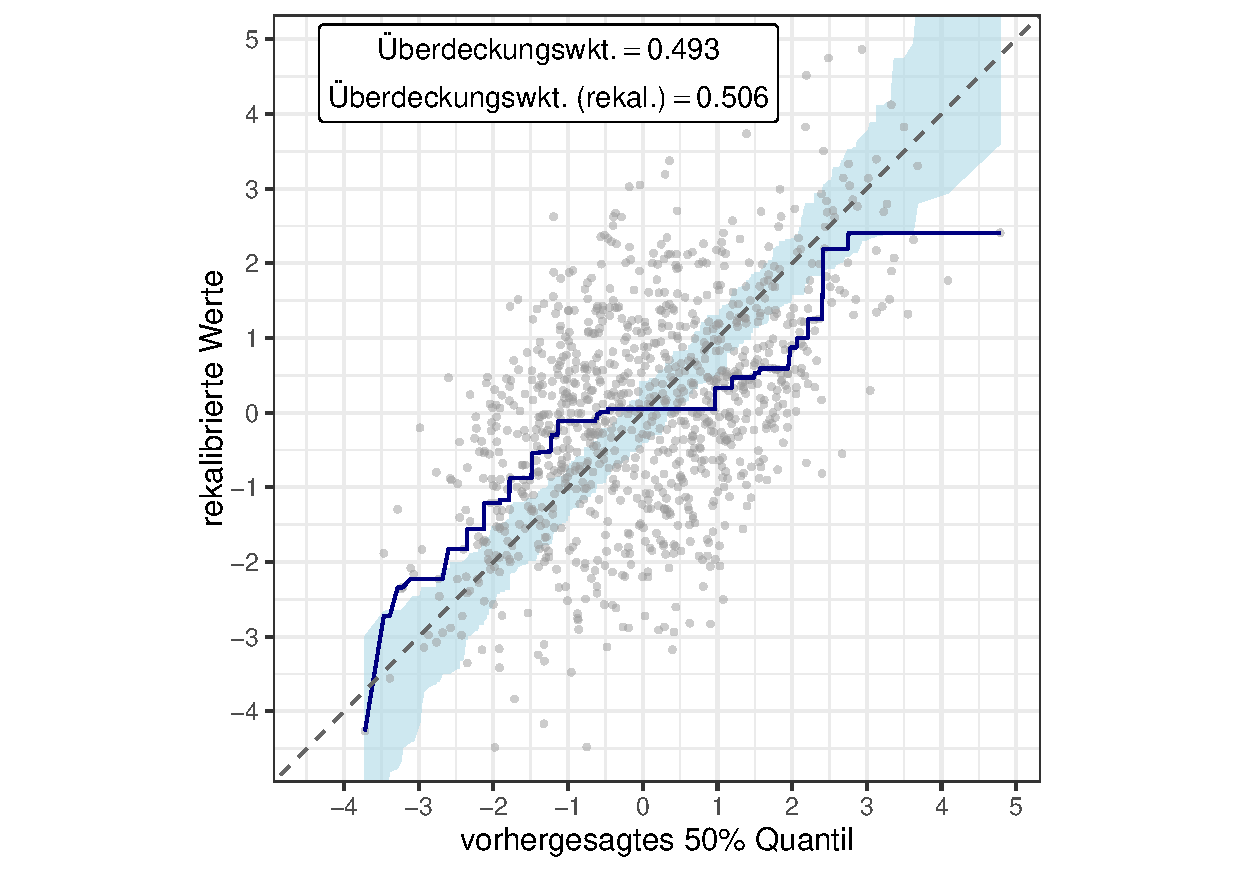
\includegraphics[width=0.7\linewidth]{figs/quant_cal.pdf}
    \caption{
    Empirisches Reliabilitätsdiagramm gemäß CORP-Ansatz für Beispiel \ref{bsp:quant_cal}. Hellblaue Bereiche entsprechen dem $95\%$-Konsistenzband basierend auf $100$ Replikationen. Punkte stellen Vorhersage-Beobachtungspaare dar.
    }
    \label{fig:quant_cal}
\end{figure}{}

Wieder können wir approzimativ Konsistenzbänder definieren unter Voraussetzung von Quantilkalibrierung. Das Verfahren ist beschrieben in \ref{sec:consistent_quant}.

Zusammenfassen können wir den CORP-Ansatz indem wir das Akronym entschlüsseln. CORP steht für Konsistent unter Annahme von Monotonie, optimally binned, reproduzierbar and PAV-based \parencite{gneiting2023regression,gneiting2023model}. PAV-based beschreibt die Methode, mit der die rekalibrierten Werte geschätzt werden, den Pool-adjacent-violator Algorithmus. Konsistent unter Monotonie, bedeutet, dass unter gültigen Voraussetzung der Monotonie das empirische Reliabilitätsdiagramm \eqref{eq:emp_rediag} ein konsistenter Schätzer für das Reliabilitätsdiagramm \eqref{eq:rediag} ist. Optimally binned, bedeutet, dass die erzeugten Bins unter den Voraussetzungen optimal bzgl. konsistenter Scoring-Functions sind, auf diese wir im Kapitel \ref{chap:scoring} näher eingehen. Reproduzierbarkeit bedeutet in diesem Zusammenhang, dass keine speziellen Hyperparameter oder Bin-Größen festgelegt werden müssen oder können, wodurch die Ergebnisse nachvollziehbar und wiederholbar bleiben.

Bislang haben wir immer \textit{ein} festes $\alpha$ betrachtet. Um Quantikalibrierung insgesamt gemäß \ref{def:all_quantcal} zu überprüfen, erstellen wir empirische Reliabilitätsdiagramme für eine ausgewählte Anzahl verschiedener  Quantileniveaus. Üblich sind die $25\%, 50\%, 75\%$ Quantile \parencite{gneiting2023model}.


\chapter{Zusammenhänge zwischen den Kalibrierungsbegriffen} \label{chap:cal_relation}
Im Folgenden beschreiben wir ausgewählte Zusammenhänge zwischen den verschiedenen Kalibrierungsbegriffen. Für eine ausführliche Aufschlüsselung der Zusammenhänge verschiedener Kalibrierungsbegriffe sei hier an \textcite{gneiting2023regression} verwiesen.

\begin{theo}[Auto-Kalibrierung impliziert marginale und probabilistische Kalibrierung \texorpdfstring{\parencite[Theorem 2.11]{gneitingCombining2013}})] \label{theo::AKthenPKMK}
Sei $F$ eine auto-kalibrierte Vorhersage bzgl. $Y$. Dann ist $F$ marginal und probabilistisch kalibriert bzgl. $Y$.
\end{theo}{}

Marginale und probabilistische Kalibrierung sind somit notwendig, aber nicht hinreichend für Auto-Kalibrierung. Auch wenn sie gemeinsam vorliegen, implizieren sie keine Auto-Kalibrierung \parencite[Example 2.4]{gneiting2023regression}.  Auch erfassen sie unterschiedliche Aspekte. So gibt es Vorhersagen, die marginal, aber nicht probabilistisch kalibriert sind sowie umgekehrt (siehe Beispiel \ref{bsp:kalunfoc}). Praktisch bedeutet es, dass wir zur Evaluation von Vorhersagen beide Kalibrierungsbedingungen überprüfen sollten.

\begin{theo}[Auto-Kalibrierung impliziert bedingte Quantilkalibrierung] \label{theo::AKthenTK}
Sei $F$ eine autokalibrierte Vorhersage bzgl. $Y$. Dann ist $F$ $\alpha$-quantilkalibriert bzgl. $Y$ für alle $\alpha \in (0,1)$
\end{theo}{}

Diese Aussage folgt aus Theorem 2.11 zusammen mit Propositon 2.18  von \textcite{gneiting2023regression} angewendet auf Quantile. Sie zeigen, dass Auto-Kalibrierung bedingte Kalibrierung für eine ganze Klasse statistischer Funktionale (Momente, Schwellenwerte, Quantile) impliziert.  Diese Klasse umfasst Funktionale, die durch sogenannte identifizierende Funktionen charakterisiert werden können.

Theorem \ref{theo::AKthenTK} und Theorem \ref{theo::AKthenPKMK} verdeutlichen, das die Auto-Kalibrierung die theoretisch stärkste Kalibrierungsbedingung ist. Die anderen Kalibrierungsbegriffe beschreiben daher Eigenschaften, die von Auto-Kalibrierung garantiert werden und ermöglichen jedoch eine empirische Untersuchung von diesen Aspekten.

Wie in Abschnitt \ref{sec:def_prob} angedeutet, sind probabilistische und unbedingte Quantilkalibrierung eng miteinander verbunden.

\begin{theo}[Probabilistische Kalibrierung impliziert unbedingte Quantilkalibrierung   \texorpdfstring{\parencite[A.5]{gneiting2023regression}})]\label{theo:pK-unbQK}
Sei $F$ eine probabilistisch kalibrierte Vorhersage bzgl. $Y$, dann ist $F$ unbedingte quantilkalibriert für alle $\alpha \in (0,1)$ bzgl. $Y$ gemäß \eqref{eq:uncond_pm_quant_cal}.\\
Sind alle Vorhersageverteilungen aus $F$ stetig und streng monoton steigend (auf gemeinsamen Träger) gilt Äquivalenz.
\end{theo}{}

Probabilistischer Kalibrierung impliziert jedoch nicht bedingte Quantilkalibrierung. Das Beispiel \ref{bsp:quant_cal} ist probabilistisch, aber nicht bedingt quantilkalibriert \parencite[Example 2.10]{gneiting2023regression}. Für die praktische Anwendung ergeben sich daraus zwei Konsequenzen: Erstens muss nach Überprüfung probabilistischer Kalibrierung die unbedingte Quantilkalibrierung nicht zusätzlich untersucht werden. Zweitens sollte vor der Untersuchung der bedingten Quantilkalibrierung zunächst die probabilistischen Kalibrierung betrachtet werden, weil sie Aufschluss über die unbedingte Quantilkalibrierung gibt.

Zusammenfassend gibt Tabelle \ref{tab:sum_kal} einen Überblick über die Kalibrierungsbegriffe, die zur empirischen Überprüfung in der vorliegenden Arbeit verwendet werden sollen.

\begin{table}[ht]
\caption{Informationsgehalt der verschiedenen Kalibrierungsbegriffe.}
\fontsize{10}{12}\selectfont
\label{tab:sum_kal}
\centering
\begin{tabularx}{\textwidth}{lXX}
\toprule
Kalibrierungsbegriff & Geprüfte Eigenschaft & Aussage bei erfüllter Kalibrierung \\
\midrule
Marginale Kalibrierung \\ &
Übereinstimmung der gemittelten Vorhersage mit Beobachtungen &
Die Vorhersage reproduziert die Marginalverteilung des Vorhersagegegenstandes.\\
\addlinespace
Probabilistische Kalibrierung \\ &
Bewertung des Gesamtbilds der vorhergesagten Verteilungen. Globale Über- bzw. Unterdispersion und systematische Verzerrung werden erkannt. &
Keine globalen Verzerrungen (Dispersion, Bias). Vorhersageintervalle werden getroffen. (Unbedingte) Quantile werden richtig vorhergesagt.\\
\addlinespace
Bedingte $\alpha$-Quantilkalibrierung\\ ($\alpha=0.25,0.5,0.75$) & Korrektheit ausgewählter Quantile bedingt auf den vorhergesagten Quantilwert. Überprüfen systematischer Fehler z.B. bei hohen bzw. niedrigen Vorhersagen. &
Die überprüften Quantile werden bedingt der Vorhersagesituation richtig getroffen. \\
\bottomrule
\end{tabularx}

\label{tab:calibration_summary}
\end{table}






 %\fi

 %\iffalse
 \chapter{Scores}\label{chap:scoring}
Möchten wir mehrere verschiedene Vorhersagen miteinander vergleichen, so ist es naheliegend, jeder Vorhersage einen einzelnen Wert zuzuordnen, der sowohl die Kalibrierung als auch die Schärfe berücksichtigt. Anhand diesen Wertes ließe sich die Qualität der Vorhersagen vergleichen und diejenige mit dem besten Wert auswählen. Dafür können wir Scores verwenden. Hierbei verwenden wir die Konvention, Scores als Verlustfunktionen zu betrachten, sodass kleinere Scores eine bessere Vorhersagegüte bedeuten. 

In Abschnitt \ref{seq:score_propertiers} definieren wir Scores und ihre Eigenschaften. Anschließend betrachten wir in Abschnitt \ref{seq:crps_qs} zwei etabilierte Scores und wie sie zusammenhängen: Den Quantilscore und den \TCRPS \;(CRPS).

Dazu bleiben wir im Vorhersageraumsetting $(F,Y)$. Zusätzlich sei $\mathcal F$ eine Familie von Wahrscheinlichkeitsverteilungen auf $\mathbb R$ mit existierendem und endlichem Erwartungswert. Sowohl die möglichen Vorhersageverteilungen als auch die bedingten Verteilungen von $Y$ bezüglich der Information $\sigma(F)$ sollen (fast sicher) in dieser Familie $\mathcal F$ liegen. Weiter nehmen wir an, dass alle auftretenden Erwartungswerte existieren und endlich sind. Wahrscheinlichkeitsverteilungen identifizieren wir mit ihren Verteilungsfunktionen. Schließlich  bezeichnen wir mit $\overline{\mathbb R}$ die erweiterten reellen Zahlen.

\section{Grundlagen und Eigenschaften} \label{seq:score_propertiers}
Je nach Anwendungsfall kann eine Vorhersage verschiedene Formen annehmen: Sie kann eine vollständige probabilistische Vorhersage sein, aber auch ein einzelner reeller Wert, etwa ein Quantil oder ein Erwartungswert. Um beide Fälle einheitlich behandeln zu können, bezeichnen wir mit $\mathcal{V}$ die Menge der möglicher Vorhersagen eines Typs. Abhängig vom Kontext gilt dann entweder $\mathcal{V} = \mathcal{F}$ oder $\mathcal{V} = \mathbb{R}$.

\begin{defi}[Score \parencite{gneitingMakingPoint2011}]
Sei $\mathcal V$ eine Menge aus einzelnen Vorhersagen. Eine Funktion
\[
S:\mathcal V\times\mathbb R\to\overline{\mathbb R},\quad (v,y)\mapsto S(v,y),
\]
heißt \emph{Scoring-Rule} bzw. \emph{Scoring-Function} oder einfach \emph{Score}, wenn sie ein Vorhersage-Beobachtungspaar $(v,y)$ auf eine Zahl abbildet.

Die obige Definition ist bewusst allgemein gehalten. Abhängig von der Art der Vorhersage $\mathcal V$ ergeben sich zwei Spezialisierungen:
\begin{itemize}
    \item $\mathcal{V}=\F$: Hierbei handelt es sich um Scoring-Rules. Es sind Scores für probabilistische Vorhersagen, bei denen vollständige Wahrscheinlichkeitsverteilungen bewertet werden. Die zentrale Eigenschaft solcher Scoring-Rules ist die \emph{Properness}.
    \item $\mathcal V=\R$: In diesem Fall entsprechen die Vorhersagen reellwertigen Punktprognosen oder statistischen Funktionalen von probabilistischen Vorhersagen. Wir nennen diese Scores; Scoring-Functions. Die zentrale Eigenschaft solcher Scoring-Functions ist die \emph{Konsistenz}. Für diese Arbeit beschränken wir uns auf Scoring-Functions für Quantile.\\
\end{itemize}
\end{defi}


\noindent
Zum Bewerten und Vergleichen von Vorhersagen bestimmen wir den erwarteten Score \parencite{gneiting2014probabilistic}.
\begin{defi}[Erwarteter Score]\label{def:exp_score}
Sei $(F,Y)$ ein Vorhersageraum und $S$ ein Score
Wir definieren den \emph{erwarteten Score} durch
\[
\bar S \coloneqq \E_\PW[S(V,Y)],
\]
wobei $V$ die jeweilige Vorhersage bezeichnet: Im Fall $\mathcal{V} = \mathcal{F}$  gilt $V = F$, im Fall $\mathcal{V} = \mathbb{R}$ gilt $V = \qF$ für ein  $\alpha$-Quantil der Verteilung $F$.
\end{defi}{}

Empirisch bestimmen wir den erwarteten Score als mittleren Score über alle Vorhersage-Beobachtungspaare, die wir betrachten \parencite{gneiting2014probabilistic}.
\begin{defi}[Empirisch erwarteter Score oder mittlerer Score]\label{def:emp_exp_score}
Für eine Stichprobe von Vorhersage-Beobachtungspaaren
$(v_i,y_i)$, $i=1,\dotsc,n$ ergibt sich der \emph{empirische erwartete Score} oder \emph{mittlerer Score}  als
\[
\hat S\coloneqq \frac1n\sum_{i=1}^n S(v_i,y_i),
\]
wobei wir je nach Art des Scores $S$ Vorhersage-Beobachtungspaare der Form \ref{eq:stich} oder \ref{eq:qaunt_stich_emp} betrachten.
\end{defi}{}
\noindent
Dieser Kennwert stellt das entscheidenende praktische Bewertungsmaß einer Vorhersage dar. Es folgen die zentralen Eigenschaften von Scores: \emph{Properness} und \emph{Konsistenz}.
\begin{defi}[Proper Score \texorpdfstring{\parencite[Definition 4]{gneiting2014probabilistic}})]
Eine Score der Form 
\[S: \F \times \R \to \overline{\R},\quad (P,y) \mapsto S(P,y)\] heißt proper relativ zu $\F$, falls für alle $P,Q \in \F$
\[
\E_{Y\sim Q}[S(Q,Y)]\leq \E_{Y\sim Q}[S(P,Y)]
\]
gilt.
\end{defi}

Properness bedeutet also, dass es im Erwartungswert optimal ist, die tatsächliche Wahrscheinlichkeitsverteilung des Vorhersagegegenstandes vorherzusagen. Jede davon abweichende Vorhersage führt zu einem mindestens ebenso großen erwarteten Score.

Hingegen ist die Konsistenz eines Scores eine Eigenschaft im Zusammenhang mit statistischen Funktionalen, etwa dem Erwartungswert, Schwellenwerten oder Quantilen \parencite[Definition 5]{gneiting2014probabilistic}. Wir beschränken uns weiterhin auf Quantile.

%mini anpassung
\begin{defi}[$\alpha$-Quantil konsistenter Score]
\label{def::consistent}
Eine Score der Form \[S: \mathbb{R} \times \mathbb{R} \to \overline{\mathbb{R}},\quad (x,y) \mapsto S(x,y)\] heißt konsistent bzgl. des $\alpha$-Quantils relativ zu $\F$, falls für alle $x \in \R$ und $Q \in \F$ 
\[
\E_{Y\sim Q}[S(q_\alpha(Q),Y)]\leq \E_{Y\sim Q}[S(x,Y)]\quad 
\]
gilt.
\end{defi}
Eine $\alpha$-quantil konsistenter Score ist somit so konstruiert, dass im Erwartungswert das wahre (bedingte) $\alpha$-Quantil optimal ist.

Die beiden Arten von Scores lassen sich ineinander überführen. So induziert ein konsistenter Score stets einen proper Score \parencite[Theorem 3]{gneitingMakingPoint2011}. Gleichzeitig zeigt sich daran, dass Properness allein als Eigenschaft nicht hinreichend für einen guten Score ist, wie im Appendix \ref{chap:other_examp} an Beispiel \ref{bsp:propernogood} deutlich wird. Daher ist es sinnvoll, auf etablierte Scores zurückzugreifen.

Im Folgenden betrachten wir zwei solcher etablierter Scores: Den \emph{Quantilscore} als $\alpha$-Quantil konsistenten Score und den \emph{\TCRPS} (CRPS) als proper Score. Dabei handelt es sich um Scores, die beide einen Minimalwert von null haben.

\section{Quantilscore und \TCRPS} \label{seq:crps_qs}
Die folgenden Scores betrachten wir relativ zur Klasse der Wahrscheinlichkeitsmaße auf $\R$ mit existierendem und endlichem Erwartungswert.

Ein konsistenter Score für das $\alpha$-Quantil ist der Quantilscore (auch Pinball Loss) \parencite[Theorem 9 (c)]{gneitingMakingPoint2011}. Er lautet
\[
\QS_\alpha(x,y) = \left(\mathds{1}\{y\le x\} - \alpha \right)(x-y)
\]
oder ausgeschrieben
\[
\QS_\alpha(x,y)=\begin{cases}
(1-\alpha)(x-y), & \text{falls } y \le x,\\[0.5em]
\alpha(y-x), & \text{falls } y > x.
\end{cases}
\]
Abhängig des gewählten $\alpha$-Quantils gewichtet der Score die Differenz $(x-y)$ zwischen beobachtetem Wert $x$ und vorhergesagtem Quantil $y$  unterschiedlich. Beim Median ist der Score symmetrisch, sodass Über- und Unterschätzungen gleich gewichtet werden. Liegt das Quantil über dem Median, werden zu niedrige Vorhersagen stärker bestraft. Liegt es unter dem Median, werden zu hohe Vorhersagen stärker bestraft. Abbildung \ref{fig:qs_visu} zeigt den Quantilscore abhängig der Differenz $(x-y)$ für das $25\%,50\%,75\%$ Quantil.


\begin{figure}[!h]
    \centering
    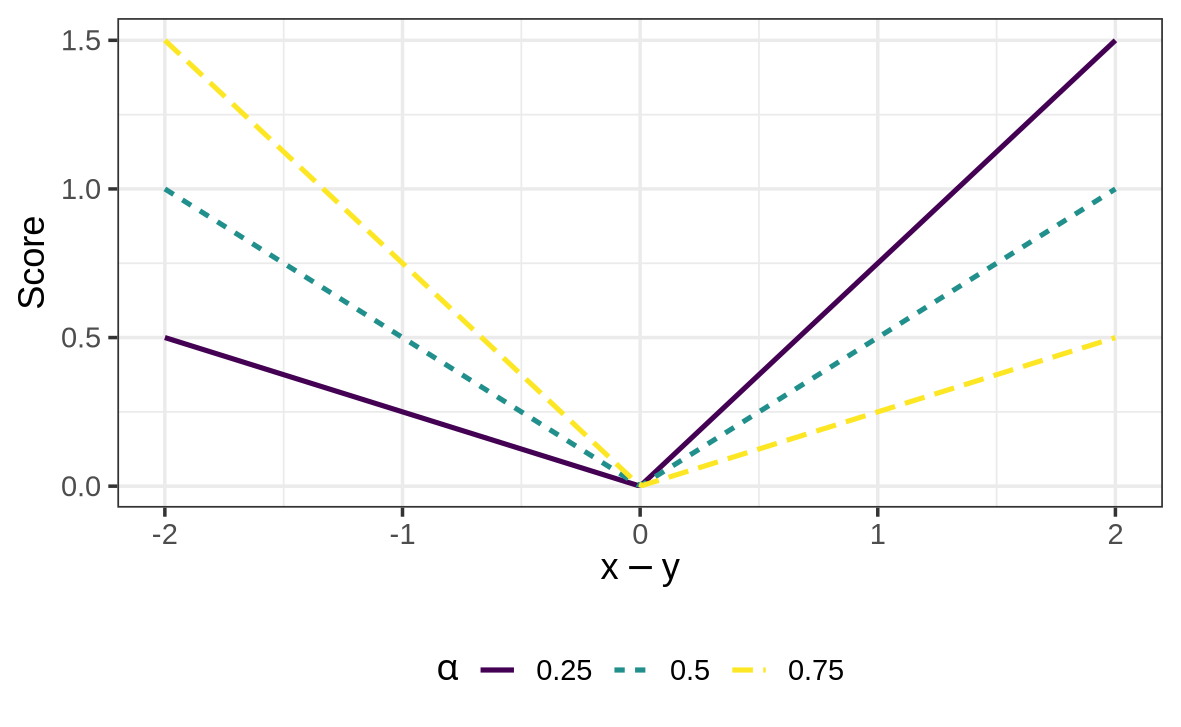
\includegraphics[width=0.75\linewidth]{figs/qs_visu_Rplot.png}
    \caption{Quantilscore abhängig der Differenz $(x-y)$ für das $25\%,50\%,75\%$ Quantil.}
    \label{fig:qs_visu}
\end{figure}

Schließlich bestimmen wir für Vorhersage-Beobachtungspaare der Form \eqref{eq:stich}  den empirischen Gesamtscore entsprechend Definition \ref{def:emp_exp_score} als
\[
\widehat{\QS}_\alpha = \frac{1}{n}\sum_{i=1}^{n}\QS_\alpha\big(q_\alpha(F_i),y_i\big).
\]
Die Höhe der erwarteten Quantilscores hängt ebenfalls vom gewählten Quantilniveau ab. Häufig werden für mittlere Quantile größere erwartete Quantilscores beobachtet als für Randquantile. Ein Grund ist jene asymmetrische Gewichtung des Quantilscores, durch die bei Randquantilen jeweils eine Fehlerseite nur gering gewichtet wird. Liegen die Vorhersagefehler überwiegend auf dieser Seite, tragen sie entsprechend nur wenig zum Quantilscore bei. Der genaue Verlauf des erwarteten Quantilscores hängt jedoch von der zugrundeliegenden Vorhersage ab.


Als nächstes führen wir den \emph{\TCRPS}$\;$(CRPS) als einen proper Score ein. Er lautet
\[
\CRPS(F,y)=\int_\R \left(F(x)-\mathds{1}\{y\leq x\}\right)^2 \,dx
\]
\parencite{Gneiting2007}. Abbildung \ref{fig:crps_visu} verdeutlicht eine geometrische Interpretation des CRPS für beispielhafte Vorhersagen.

\begin{figure}[!h]
    \centering
    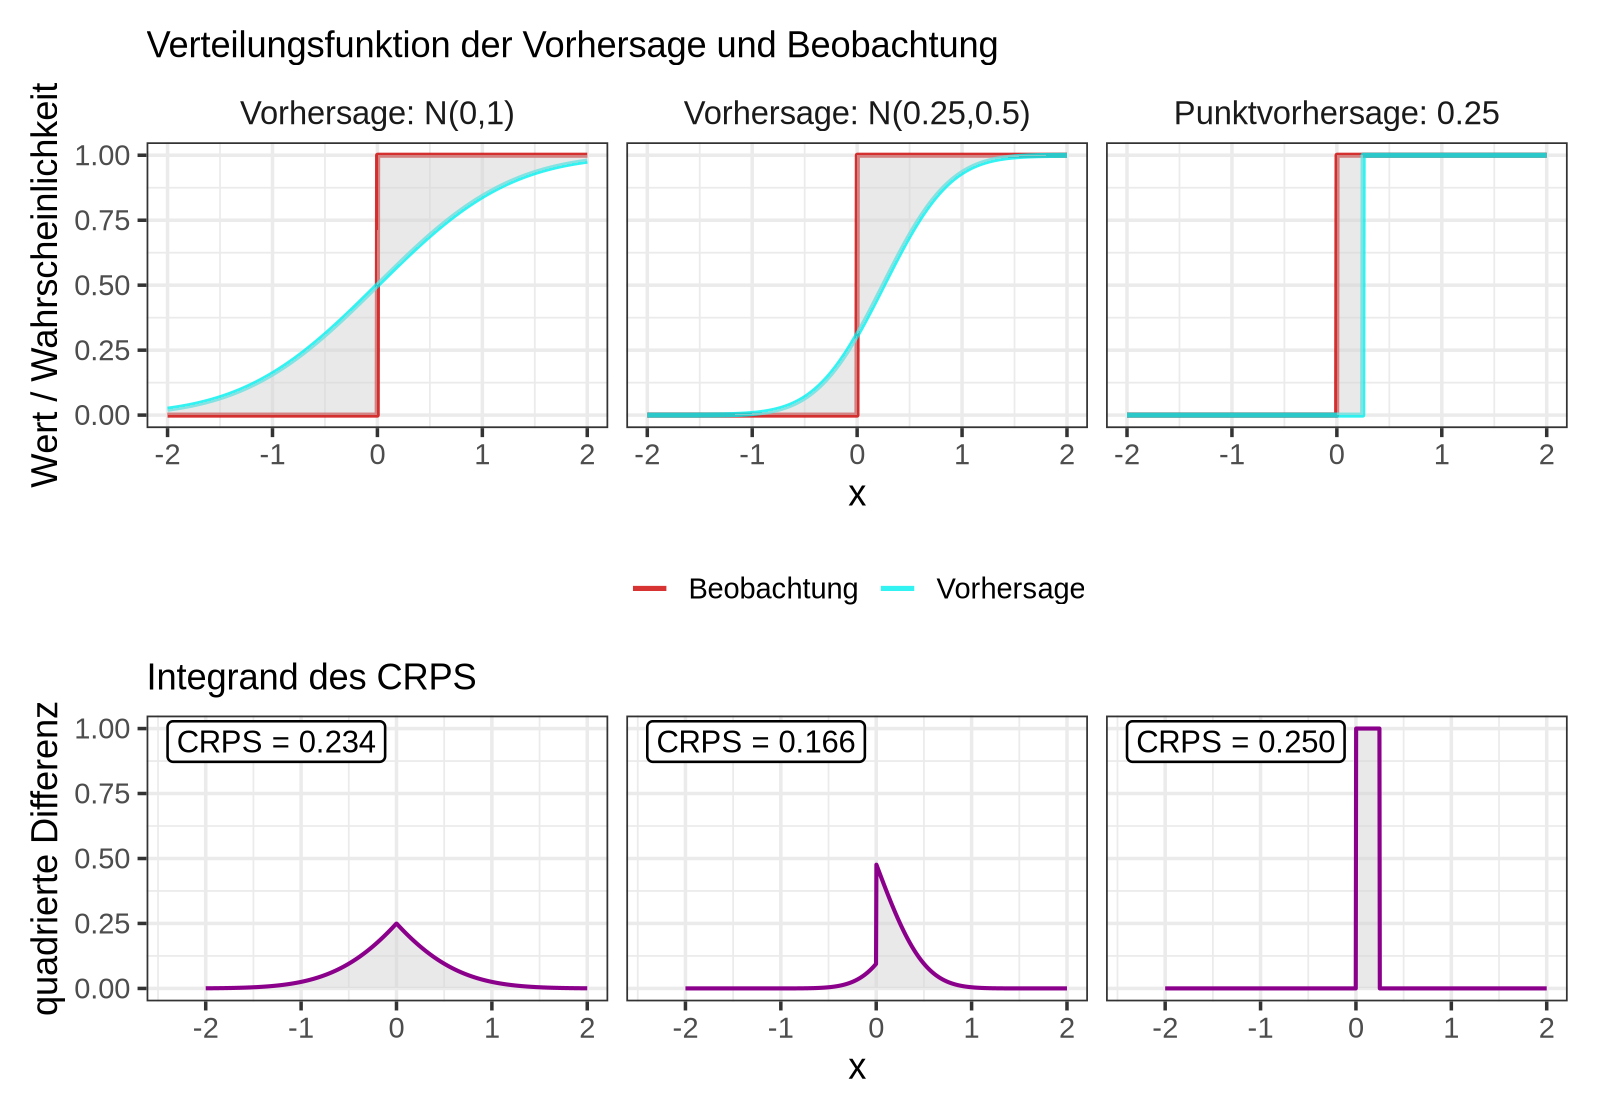
\includegraphics[width=\linewidth]{figs/crps_visu_Rplot.png}
    \caption{CRPS Visualisierung für verschiedene Vorhersagen. Oben wird die Vorhersageverteilungsfunktion mit einer Beobachtung von Wert 0 verglichen. Die Beobachtung ist als Indikatorfunktion dargestellt. Die graue Fläche markiert die Abweichung zwischen beiden Funktionen. Unten ist diese Abweichung für jeden Wert von x quadriert dargestellt. Das Integral über diese quadrierte Differenz ergibt den CRPS.}
    \label{fig:crps_visu}
\end{figure}


Er besitzt mehrere Eigenschaften, die ihn für die Bewertung probabilistischer Vorhersagen attraktiv machen. Erstens benötigen wir, dadurch dass er auf Verteilungsfunktionen basiert, zur Anwendung keine Kenntnisse über die zugehörige Dichtefunktion, was in einigen Anwendungen hilfreich seien kann. Zum anderen reduziert er sich im Fall einer Punktvorhersage (dargestellt als Punktmaß) auf den absoluten Fehler $\abs{x-y}$  \parencite{Gneiting2007}, wie auch in Abbildung \ref{fig:crps_visu} erkennbar ist. Dadurch ist er eine natürliche Verallgemeinerung klassischer Fehlermaße und ermöglicht somit einen direkten Vergleich zwischen Punktvorhersage und probabilistischer Vorhersage. Schließlich liegt der CRPS in derselben Einheit wie die vorhergesagte Größe vor, was seine Interpretation erleichtert.

Den empirischen Gesamtscore bestimmen wir analog zum Quantilscore für Paare der Form \eqref{eq:stich} als
\[
\widehat{\mathrm{CRPS}} = \frac{1}{n}\sum_{i=1}^{n}\CRPS(F_i,y_i).
\]
Um den CRPS zu berechnen, können wir je nach Verteilung, numerische Methoden oder analytische Formen verwenden. Im Allgemeinen sind keine geschlossenen analytischen Ausdrücke verfügbar. Für eine Vielzahl von Verteilungen gibt es diese jedoch \parencite{scoringRules}. Zur Bestimmung solcher Ausdrücke kann folgende alternative Darstellung des CRPS hilfreich sein \parencite{Gneiting2007}: 
\[
\CRPS(F,y)=\mathbb{E}\abs{X-y}-\frac{1}{2}\E\abs{X-X'},\qquad X,X' \overset{\text{i.i.d.}}{\sim} F.
\]
Mit ihr ergibt sich beispielsweise für eine empirische Verteilungsfunktion $F_m$, erzeugt aus Werten $z_1,\dotsc, z_m$ der CRPS als \parencite{scoringRules}
\begin{equation} \label{eq:crps_emp}
\CRPS(F_m,y)= \frac{1}{m}\sum_{i=1}^m\abs{z_i-y}-\frac{1}{2m^2} \sum_{i=1}^m\sum_{j=1}^m\abs{z_i-z_j}.
\end{equation} Für eine Normalverteilung erhaltenen wir
\[
\CRPS\bigl(\mathcal{N}(\mu,\sigma^2), x\bigr)
=
\sigma
\left[
z\left(2\Phi(z)-1\right)
+2\varphi(z)
-\frac{1}{\sqrt{\pi}}
\right]
\quad  \text{mit} \quad
z=\frac{x-\mu}{\sigma},
\]
wobei $\varphi$ die Dichte und $\Phi$ die Verteilungsfunktion der Standardnormalverteilung bezeichnen \parencite{gneiting2014probabilistic}. 


Abschließen führen wir eine weitere Darstellung des CRPS ein, mit der wir einen direkten Bezug zum Quantilscore herstellen. Sie stammt von \textcite{TameaQSCRPS} und lautet
\begin{equation} \label{eq:crps_qs}
\CRPS(F,y)=2\int_0^1 \QS_\alpha(q_\alpha(F),y)\,d\alpha.    
\end{equation}

Der CRPS lässt sich somit als Integral des Quantilscores über alle Quantilniveaus interpretieren. Daraus können wir ein einfache Approzimation des CRPS durch diskretisieren des Integrals an einer endlichen Menge von Quantilen erhalten. Diese Approzimation ist äquivalent zu einer weiteren proper Scoring-Rule dem \emph{Weighted Interval Score}, der probabilistische Vorhersagen anhand mehrerer symmetrisch um den Median gewählter Quantile bewertet \parencite{FakoorQSCRPS}.

Außerdem ermöglicht die Darstellung des CRPS als Quantilscore eine effiziente Berechnung für empirische Verteilungsfunktionen. Für eine empirische Verteilungsfunktion $F_m$ erzeugt aus Werten $z_1 \le \dotsc \le z_m$ können wir den $\CRPS$ folgendermaßen darstellen
\begin{equation} \label{eq:crps_qs_emp}  
\CRPS(F_m,y)=\frac{2}{m}\sum_{k=1}^m (\mathds{1}\{y \le z_k\}-\alpha_k) (z_k-y) \quad \text{mit} \quad \alpha_k=\frac{2k-1}{2m}.
\end{equation} Diese Berechnungsvorschrifft wird beispielsweise standardmäßig im R-Paket \texttt{scoringRules} genutzt \parencite{scoringRules}.




Zusätzlich erhalten wir mit der Darstellung des CRPS über den Quantilscore eine Möglichkeit, ihn besser zu untersuchen, indem wir den verdoppelten erwarteten Quantil\-score in Ab\-hängig\-keit vom Quantil\-niveau darstellen. Die Fläche unter der Kurve entspricht dabei dem erwarteten CRPS, sodass wir erkennen können, welche Quantilbereiche zu dessen Wert beitragen. Beim Vergleich mehrerer Vorhersagen ist eine Vorhersage in einem Quantilbereich besser, wenn ihre Quantilscorekurve unter derjenigen der anderen Vorhersage liegt. Typischerweise erhalten wir einen umgekehrt U-förmigen Verlauf, sodass die mittleren Quantilscores den größten Beitrag zum CRPS leisten, während die Randquantile geringere Scores aufweisen. Eine ähnliche Darstellung verwenden \textcite{Gneiting2007} in Fig. 10, in der der Brier Score (eine konsistente Scoring-Function) in Abhängigkeit vom Schwellenwert dargestellt wird. Sie bezeichnen diese Abbildung als \emph{Prediction-Error-Curve}. In Anlehnung daran bezeichnen wir unsere Darstellung des Quantilscores als \emph{Quantile-Error-Curve}.

\begin{bsp}[Quantile-Error-Curve] \label{bsp:quantile-error-curve}
Wir stellen die Quantile-Error-Curve für den Vorhersagegenstand aus Beispiel \ref{bsp:auto_kal} hinsichtlich der Vorhersagen $F_1,F_2,F_3$ (die ideale, marginale und unfokussierte Vorhersage) aus den Beispielen \ref{bsp:auto_kal} und \ref{bsp:quant_cal} dar.

Abbildung \ref{fig:quantile-error-curve} zeigt die Quantile-Error-Curve der Vorhersagen auf Basis einer Simulation mit $3000$ Stichproben. Wir erkennen einen umgekehrt U-förmigen Verlauf der Quantilscorefunktionen. Dabei ist die Kurve der idealen Vorhersage am niedrigsten in allen Quantilbereichen und weist daher den niedrigsten CRPS auf. Für die marginale und die unfokussierte Vorhersage zeigen sich nahezu identische Kurven, wobei die marginale Vorhersage im mittleren Quantilbereich minimal besser und im äußeren Quantilbereich minimal schlechter ist. Hinsichtlich des CRPS bedeutet das, dass beide Vorhersagen einen ähnlichen Wert haben.
\end{bsp}

\begin{figure}
    \centering
    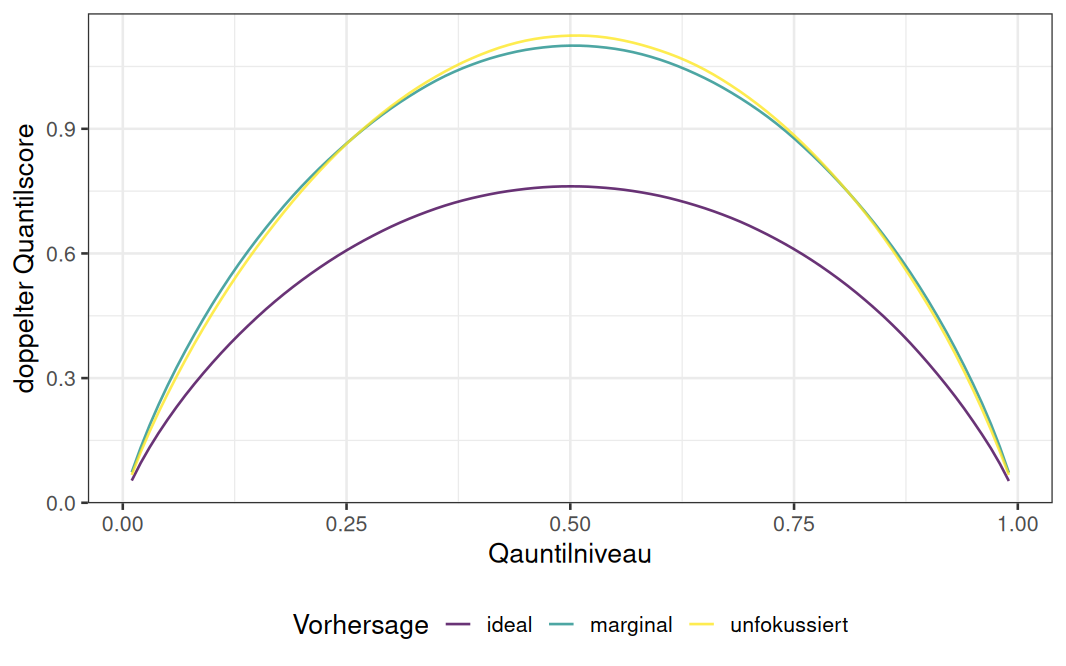
\includegraphics[width=.8\linewidth]{figs/qs_crps_visu_Rplot.png}
    \caption{Quantile-Error-Curve für Beispiel \ref{bsp:quantile-error-curve}
    }
    \label{fig:quantile-error-curve}
\end{figure}{}

Schließlich ist die Darstellung des CRPS über den Quantilscore besonders hilfreich, wenn wir im Folgenden den CRPS in verschiedene Komponenten zerlegen. 





\chapter{Score Zerlegung}  \label{chap:score_decomp}
Wie im vorherigen Kapitel beschrieben ist ein Vorteil von Scores, dass wir mit ihnen eine Vorhersage anhand einer einzigen Zahl bewerten können, was leicht einen Vergleich verschiedener Vorhersagen ermöglicht. Gleichzeitig bleibt zunächst unklar, auf welche Eigenschaften einer Vorhersage der jeweilige Score tatsächlich zurückzuführen ist. Denn Scores berücksichtigen sowohl die Kalibrierung als auch die Schärfe einer Vorhersage \parencite{gneiting2014probabilistic}. Ein guter Score kann daher sowohl aus einer guten Kalibrierung als auch aus einer hohen Schärfe resultieren. Umgekehrt kann ein schlechter Score aus Defiziten in einem oder beiden dieser Aspekte entstehen.

Aus diesem Grund ist es sinnvoll, Scores in einzelne Komponenten zu zerlegen, die Kalibrierung und Schärfe getrennt erfassen. Das ermöglicht eine differenziertere Analyse der Vorhersagequalität und macht transparent, welche Aspekte einer Vorhersage zu ihrem Score beitragen. Entsprechend können Anwender diejenige Vorhersage wählen, die am besten zu ihren Ansprüchen passt. Beispielsweise kann in Anwendungen, in denen verlässliche Wahrscheinlichkeitsaussagen im Vordergrund stehen, eine gut kalibrierte Vorhersage bevorzugt werden, selbst wenn diese geringere Schärfe oder sogar einen insgesamt schlechteren Score als Alternativen aufweist.

In diesem Kapitel geht es daher primär um die Zerlegung des Quantilscores und des CRPS gemäß \textcite{gneiting2023regression} und \textcite{arnold2024decompositions}. In Abschnitt \ref{seq:score_components} beschreiben wir zunächst allgemein die Komponenten und die Idee hinter der Zerlegung, bevor wir sie in Abschnitt \ref{seq:decomp_qs} anhand der Zerlegung des Quantilscores verdeutlichen.  Für die empirische Umsetzung greifen wir auf den in Abschnitt \ref{sec:emp_prüf_quantcal} vorgestellten CORP-Ansatz zur Quantilkalibrierung zurück. Aufbauend auf dieser Zerlegung erläutern wir in Abschnitt \ref{seq:decomp_crps} eine Zerlegung des CRPS, wobei der Fokus auf der empirischen Umsetzung liegt. Anschließend stellen wir in Abschnitt \ref{seq:decomp_visu} eine Möglichkeit zur Visualisierung der Zerlegungen und in Abschnitt \ref{seq:decomp_skill} mit dem Skill Score eine Möglichkeit zur relativen Einordnung von Scores vor. Abschließend beschreiben wir in Abschnitt \ref{seq:decomp_prop} Eigenschaften, die wir uns von Scorezerlegungen wünschen könnem, und dass die in dieser Arbeit verwendeten Zerlegungen des Quantilscores und des CRPS diese Eigenschaften erfüllen.

\section{Komponenten der Zerlegung} \label{seq:score_components}
Gemäß \textcite{gneiting2023regression} erfolgt die Zerlegung eines Scores in drei Komponenten: Unsicherheit, Diskriminationsfähigkeit und Misskalibrierung. Die Unsicherheit (UNC) beschreibt die inhärente Variabilität des Vorhersagegegenstands. Sie ist damit keine Eigenschaft der Vorhersage und kann daher nicht durch Verbesserung dieser reduziert werden. Je höher der Wert, desto größer die Variabilität des Vorhersagegegenstands. Die Diskriminationsfähigkeit (DSC) bezeichnet die Fähigkeit einer Vorhersage, unterschiedliche Situationen zu unterscheiden. Sie entspricht dem Informationsgehalt der Vorhersage und erfasst damit die Schärfe der Vorhersage. Je größer der Wert, desto besser ist die Diskriminationsfähigkeit einer Vorhersage. Die Misskalibrierung (MCB) misst fehlende Kalibrierung. Ein hoher Wert deutet auf schlechte Kalibrierung hin. Für einen erwarteten Score $\bar S$ erhalten wir die Zerlegung
\[
\bar S = \MCB - \DSC + \UNC.
\]

Nun stellt sich die Frage, wie sich diese Komponenten bestimmen lassen. Grundlegend vergleichen wir hierzu den erwarteten Score der ursprünglichen Vorhersage mit den Scores einer marginalen und einer rekalibrierten Referenzvorhersage. Während die marginale Referenzvorhersage auf der marginalen Verteilung des Vorhersagegegenstandes basiert, basiert die rekalibrierte Referenzvorhersage auf dessen bedingter Verteilung gegeben die ursprüngliche Vorhersage. Das Vorgehen wird im Folgenden zunächst am Beispiel der Quantilscorezerlegung verdeutlicht.

\section{Zerlegung des Quantilscores} \label{seq:decomp_qs}
Wir beschreiben die Zerlegung des Quantilscores nach \textcite{gneiting2023regression}. Wie für $\alpha$-Quantilkalibrierung betrachten wir für ein $\alpha \in (0,1)$ das Paar \eqref{eq:qaunt_stich_pop} sowie Vorhersage-Beobachtungspaare der Gestalt \eqref{eq:qaunt_stich_emp}. Zusätzlich führen wir die zur Zerlegung benötigten Referenzvorhersagen ein. Mit 
\[
x_0 \coloneqq q_\alpha(Y)
\] 
bezeichnen wir das marginale $\alpha$-Quantil des Vorhersagegegenstandes $Y$, welches die marginale Referenzvorhersage darstellt.
Wir bezeichnen mit
\[
X_{\mathrm{rc}} \coloneqq q_\alpha(Y \mid q_\alpha(F))
\]
die rekalibrierte Quantilvorhersage. $X_\rc$ gibt also an, wie das vorhergesagte Quantil angepasst werden müsste, damit es, bedingt auf jenes, das tatsächliche Quantil von $Y$ korrekt trifft. Entsprechend gilt, sofern $X=X_\rc$ fast sicher ist, dass die Vorhersage bedingt $\alpha$-quantilkalibriert entsprechend der Gleichung \eqref{eq:cond_alpha_quant_cal} ist. Umgekehrt deuten Abweichungen zwischen diesen Größen auf Defizite in der Kalibrierung hin.

%Im Rahmen des Vorhersageraums sind $X$ und $X_{\mathrm{rc}}$ im Allgemeinen Zufallsvariablen, während $x_0$ eine deterministische Größe ist.
Damit haben wir nun folgende drei Vorhersagen: Die eigentlichen Quantilvorhersagen $X$, die rekalibrierte Quantilvorhersage $X_\rc$ sowie die marginale Referenzvorhersage $x_0$. Für diese bestimmen wir nun die erwarteten Scores gemäß Definition \ref{def:exp_score} und nennen diese den (erwarteten) Gesamtscore $\overline{\QS}_\alpha$, den rekalibrierten Score $\overline{\QS}^{\rc}_\alpha$ und den marginalen Score $\overline{\QS}^{\mg}_\alpha$. Sie lauten also
\[
\overline{\QS}_\alpha \coloneqq \E_\PW[\QS_\alpha(X,Y)], \quad
\overline{\QS}^{\rc}_\alpha \coloneqq \E_\PW[\QS_\alpha(X_{\rc},Y)], \quad
\overline{\QS}^{\mg}_\alpha \coloneqq \E_\PW[\QS_\alpha(x_0,Y)].
\]
Mit diesen Scores können wir nun die Zerlegungskomponenten bestimmen. Sie sind definiert als
\[
\MCB_\alpha \coloneqq \overline{\QS}_\alpha - \overline{\QS}^{\rc}_\alpha, \quad
\DSC_\alpha \coloneqq \overline{\QS}^{\mg}_\alpha - \overline{\QS}^{\rc}_\alpha, \quad
\UNC_\alpha \coloneqq \overline{\QS}^{\mg}_\alpha.
\]
Diese Definitionen spiegeln direkt die inhaltliche Interpretation der drei Komponenten wider: Die Misskalibrierung entspricht der Verbesserung der Vorhersage durch Rekalibrierung, die Diskriminationsfähigkeit den zusätzlichen Informationsgehalt der rekalibrierten gegenüber der marginalen Referenz und die Unsicherheit dem erwarteten Score der marginalen Referenzvorhersage.
Damit haben wir die Zerlegung
\[
\overline{\QS}_\alpha = \MCB_\alpha - \DSC_\alpha + \UNC_\alpha
\]
erhalten.

Auf empirischer Ebene besteht die Herausforderung darin, die rekalibrierten 
Werte $X_{\mathrm{rc}}$ zu bestimmen. Der in Abschnitt \ref{sec:emp_prüf_quantcal} beschriebene 
CORP-Ansatz liefert solche Schätzer mittels des PAV-Algorithmus. Konkret setzen 
wir
\[
\hat{x}_i = \hat{q}_\alpha(Y \mid X = x_i)
\quad \text{und} \quad
\hat{x}_0 = \hat{q}_\alpha(Y),
\]
wobei $\hat{q}_\alpha(Y)$ das empirische $\alpha$-Quantil der Beobachtungen 
und $\hat{x}_i$ die rekalibrierten Qauntile des CORP-Ansatzes bezeichnet. Die empirischen Scores sind dann gegeben durch
\begin{equation} \label{eq:decomp_qs_emp_scores}
\widehat{\QS}_\alpha \coloneqq \frac{1}{n}\sum_{i=1}^{n}\QS_\alpha(x_i,y_i), \;\;
\widehat{\QS}^{\rc}_\alpha \coloneqq \frac{1}{n}\sum_{i=1}^{n}\QS_\alpha(\hat{x}_i,y_i), \;\;
\widehat{\QS}^{\mg}_\alpha \coloneqq \frac{1}{n}\sum_{i=1}^{n}\QS_\alpha(\hat{x}_0,y_i),
\end{equation}
sodass die empirische Zerlegung
\[
\widehat{\QS}_\alpha = \widehat{\MCB}_\alpha - \widehat{\DSC}_\alpha + \widehat{\UNC}_\alpha
\]
mit
\[
\widehat{\MCB}_\alpha \coloneqq \widehat{\QS}_\alpha - \widehat{\QS}^{\rc}_\alpha, \quad
\widehat{\DSC}_\alpha \coloneqq \widehat{\QS}^{\mg}_\alpha - \widehat{\QS}^{\rc}_\alpha, \quad
\widehat{\UNC}_\alpha \coloneqq \widehat{\QS}^{\mg}_\alpha
\]
lautet. 

\section{Zerlegung des CRPS auf Basis des Quantilscores} \label{seq:decomp_crps}
Im Gegensatz zu Scoring-Functions wie dem Quantilscore ist die Zerlegung für Scoring-Rules wie dem CRPS komplizierter. Wieder benötigen wir zur Zerlegung eine marginale und eine rekalibrierte Referenzvorhersage. Im Gegensatz zum Quantilscore handelt es sich bei diesen Referenzvorhersagen jedoch nicht mehr nur um Punktvorhersagen, sondern um probabilistische Vorhersagen. Zudem ist die rekalibrierte Referenzvorhersage stets an einen bestimmten Kalibrierungsbegriff gebunden. Bei der Zerlegung des Quantilscores für das $\alpha$-Quantil ergab sich hierfür die (bedingte) $\alpha$-Quantilkalibrierung als natürliche Bedingung. Für den CRPS wäre daher eigentlich, weil wir mit ihm gesamte Vorhersageverteilungen bewerten, die Auto-Kalibrierung der natürliche Kalibrierungsbegriff. In diesem Fall lautete die marginale Referenzvorhersage
\begin{equation}\label{eq:marg_ref_crps}
    F_0 \coloneqq \LW(Y)
\end{equation}
und die rekalibrierte Referenzvorhersage 
\[
F_\rc\coloneqq \LW \left(Y \mid F \right).
\] 
Eine Zerlegung des CRPS hinsichtlich der Auto-Kalibrierung erweist sich jedoch empirisch als wenig geeignet (Begründung in Abschnitt \ref{seq:decomp_prop}). Alternativ kann der CRPS auch hinsichtlich anderer Kalibrierungsbegriffe zerlegt werden. Hierfür lassen sich äquivalente Darstellungen des CRPS verwenden. Eine Möglichkeit ist die Zerlegung hinsichtlich Quantilkalibrierung (Definition \ref{def:all_quantcal}) für die wir die Darstellung des CRPS über den Quantilscore \eqref{eq:crps_qs} verwenden können. 
Diese Zelegung gemäß \textcite{arnold2024decompositions} wird im Folgenden aufgeführt. Im Gegensatz zur Quantilscorezerlegung beschränken wir uns hier auf die empirische Umsetzung, weil wir die entsprechenden Populationsterme analog konstruieren können.

Die Grundidee besteht darin, dass wir durch die Darstellung des CRPS als Integral der Quantilscores \eqref{eq:crps_qs} die Rekalibrierung auf die Ebene der einzelnen Quantile verlagern können. Somit umgehen wir zugleich die direkte Konstruktion probabilistischen Referenzvorhersagen. Stattdessen führen wir die bereits für den Quantilscore entwickelte Zerlegung für mehrere Quantile separat durch und übertragen sie anschließend auf den CRPS. 


%Somit umgehen wir zugleich die direkte Konstruktion probabilistischen Referenzvorhersagen und ¨ubertragendie Zerlegung des Quantilscores ¨uber die Quantildarstellung auf den CRPS direkt
Für Vorhersage-Beobachtungspaare der Form \eqref{eq:stich} schreiben wir mit \eqref{eq:crps_qs} und \eqref{eq:decomp_qs_emp_scores} den empirischen Gesamtscore als
\begin{equation}\label{eq:decomp_crps}
    \widehat{\CRPS}= \frac{1}{n}\sum_{i=1}^{n} 2\!\int_0^1 \QS_\alpha(q_\alpha(F_i),y_i)\,d\alpha = 2 \int_0^1\widehat{\QS}_\alpha \,d\alpha.
\end{equation} 
Aufgrund dieser Darstellung können wir den marginalen und den rekalibrierten Score analog aus den entsprechenden Quantilscores konstruieren:
\begin{equation} \label{eq:decomp_crps_scores}
  \widehat{\CRPS}^{\rc}=2 \int_0^1\widehat{\QS}^{\rc}_\alpha \,d\alpha, \quad \quad
  \widehat{\CRPS}^{\mg}=2 \int_0^1\widehat{\QS}^{\mg}_\alpha \,d\alpha .
\end{equation}
Für den rekalibrierten Score nutzen wir also die durch den CORP-Ansatz bestimmten rekalibrierten bedingten Quantile als Vorhersagen und für den marginalen Score die Quantile der Beobachtungen als Vorhersagen. So erlangen wir
\[
\widehat{\CRPS} = \widehat{\MCB} - \widehat{\DSC} + \widehat{\UNC}\\
\]
mit
\[
\widehat{\MCB}=\widehat{\CRPS} - \widehat{\CRPS}^{\rc}, \quad
\widehat{\DSC}=\widehat{\CRPS}^{\mg} - \widehat{\CRPS}^{\rc}, \quad
\widehat{\UNC}= \widehat{\CRPS}^{\mg}\;
\]

Zur Berechnung der verschiedenen Scores \eqref{eq:decomp_crps} und \eqref{eq:decomp_crps_scores} müssen Integrale gelößt werden. Diese approximieren wir numerisch. Dazu verwenden wir in der vorliegenden Arbeit die Gauß-Legendre-Quadratur \parencite{gautschi2004orthogonal} mit 25 Stützstellen auf dem Intervall $[0,1]$. Bezeichnen $(\alpha_k,w_k)^{25}_{k=1}$ die zugehörigen Stützstellen und Gewichte, so approximieren wir
\begin{align}
    \widehat{\CRPS}& = 2\int_0^1\widehat{\QS}_\alpha \,d\alpha \approx 2 \sum_{k=1}^{25}w_k\, \widehat{\QS}_{\alpha_k}  \\
    \widehat{\CRPS}^{\rc}&=2 \int_0^1\widehat{\QS}^{\rc}_\alpha \,d\alpha \approx 2 \sum_{k=1}^{25}w_k\, \widehat{\QS}^{\rc}_{\alpha_k}
\end{align}
Für den erwarteten rekalibrierten Score bestimmen wir also für alle Stützstellen $\alpha_k$ die rekalibrierten Quantile mithilfe des CORP-Ansatzes.

Für empirische Vorhersageverteilungen erfolgt die Berechnung des CRPS hingegen direkt über die Darstellung \eqref{eq:crps_qs_emp}, sodass keine numerische Quadratur erforderlich ist. Für den erwarteten rekalibrierten Score bestimmen wir dann die rekalibrierten Quantile für die Niveaus
\[
\alpha_k=\frac{2k-1}{2m},\qquad k=1,\dots,m,
\]
wobei $m$ die Anzahl der Werte der empirischen Vorhersageverteilung bezeichnet.



Aufgrund der unterschiedlichen Berechnungsmethoden können beim Vergleich von Vorhersagen auf Basis empirischer Vorhersageverteilungen mit Vorhersagen auf Basis stetiger Verteilungsfunktionen numerische Abweichungen im marginalen Score auftreten. Das ist insofern problematisch, da der marginale Score die Unsicherheitskomponente der Zerlegung bestimmt, die ausschließlich auf dem Vorhersagegegenstand beruht und somit für alle Vorhersagen identisch sein sollte. Um solche numerischen Abweichungen zu vermeiden, verwenden wir daher eine einheitliche alternative Berechnungsmethode für den marginalen Score bzw. die Unsicherheitskomponente. Die folgende Aussage liefert die Grundlage für diese Berechnung.

\begin{theo}[Marginaler Score der CRPS-Quantilscorezerlegung entpricht marginalem Score der Zerlegung bzgl. Autokalibrierung \texorpdfstring{\parencite[Proposition 2.2]{arnold2024decompositions}})] \label{theo:crps_mg_eqi}
    \[
        \widehat{\CRPS}^{\mg}=2 \int_0^1\widehat{\QS}^{\mg}_\alpha \,d\alpha = \frac{1}{n}\sum_{i=1}^n \CRPS\left(\widehat{\PW}(Y \leq \cdot) ,y_i\right),
    \]
     wobei  $\;\widehat{\PW}(Y \leq \cdot)$ entsprechend \eqref{eq:Y_mg}, die empirische marginale Verteilung des Vorhersagegegenstandes beschreibt und damit die empirische Variante der marginalen Referenzvorhersageverteilung $F_0$ \eqref{eq:marg_ref_crps} darstellt .
\end{theo}
Das heißt, bei der Quantilscorezerlegung entspricht der marginale Score dem mittleren CRPS der empirischen marginalen Verteilung des Vorhersagegegenstandes. Dadurch lässt sich die $\widehat{\UNC}$-Komponente unabhängig von der Berechnungsmethode einheitlich darstellen und effizient berechnen mit:
\begin{align*}
\widehat{\CRPS}^{\mg}&=2 \int_0^1\widehat{\QS}^{\mg}_\alpha \,d\alpha \\
                    &= \frac{1}{n}\sum_{i=1}^n \CRPS\left(\widehat{\PW}(Y \leq \cdot),y_i\right) && ,\text{Theorem \ref{theo:crps_mg_eqi}}\\ %theorem
                    &= \frac{1}{n}\sum_{i=1}^n\left[\frac{1}{n}\sum_{j=1}^n\abs{y_j-y_i}-\frac{1}{2n^2} \sum_{k=1}^n\sum_{j=1} ^n\abs{y_k-y_j}\right] && ,\text{\eqref{eq:crps_emp}}\\ %empirische rgel
                    &= \frac{1}{2n^2}\sum_{k=1}^n\sum_{j=1}^n\abs{y_k-y_j} \\
                    &= \frac{1}{n^2}\sum_{k=1}^n(2k-n-1)\cdot y_k. %hier noch die Rechenvorschrift
\end{align*}
Die letzte Gleichheit folgt aus der Darstellung der Summe absoluter Differenzen für aufsteigend sortierte Beobachtungen, wobei für die Gültigkeit die $y_k$ aufsteigend sortiert sein müssen.











\section{Darstellen der Score Zerlegung} \label{seq:decomp_visu}
%gucken das miskalibrierung mit einem s geschriebnen
Zu visuellen Darstellung einer Score Zerlegung orientieren wir und an \textcite{gneiting2023model} und \textcite{arnold2024decompositions}. Dazu bilden wir auf der x-Achse die Miskalibrierung (MCB) und auf der y-Achse die Diskriminationsfähikeit (DSC) verschiedener Vorhersagen ab. Höhenlinien zeigen gleiche erwartete Scores. Je weiter links ein Punkt liegt, desto besser ist eine Vorhersage kalibriert, je höher eine Vorhersage liegt desto besser ist ihre Diskriminationsleistung. Damit sind die besten Vorhersagen oben links in der Darstellung. Zusätzlich stellen wir die UNC-Komponente im Plot dar, sodass die erwarteten Scores der Vorhersagen direkt mit dem marginalen Referenzscore verglichen werden können. Die Darstellung ermöglicht es insbesondere, mehrere Vorhersagen gleichzeitig hinsichtlich ihrer Score Komponenten zu vergleichen. Dadurch werden die unterschiedlichen Eigenschaften der Vorhersagen unmittelbar zueinander in Beziehung gesetzt. Das folgende Beispiel verdeutlicht die Darstellung.

\begin{figure}[!h]
    \centering
    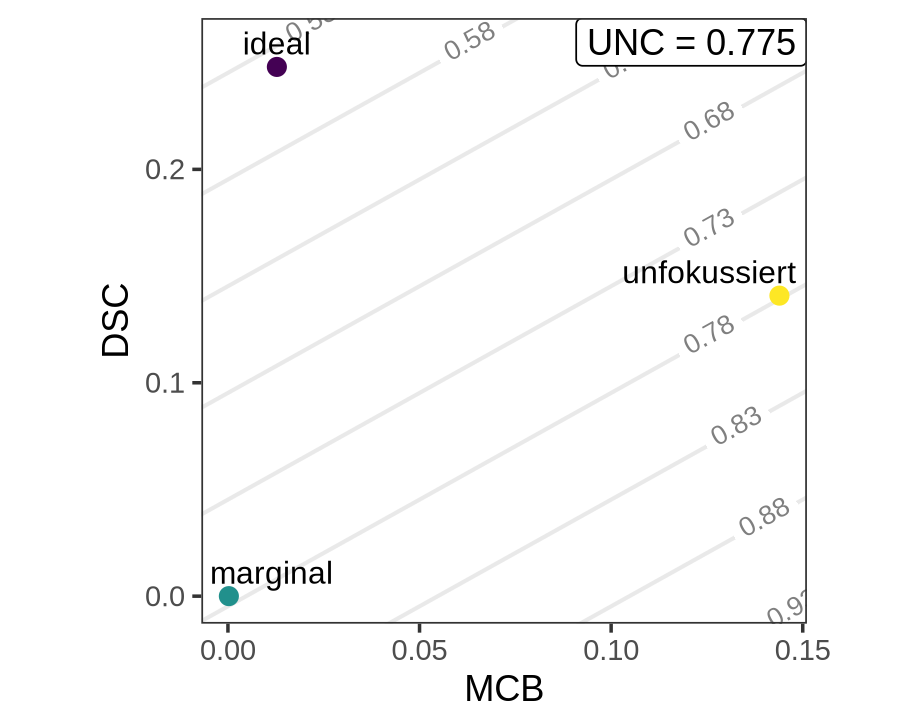
\includegraphics[width=0.55\linewidth]{figs/decomp_visu_Rplot.png}
    \caption{CRPS Zerlegungsdiagramm für das Beispiel \ref{bsp:crps_decomp}.}
    \label{fig:decomp_visu}
\end{figure}

\begin{bsp}[Mehrwert durch Score Zerlegung] \label{bsp:crps_decomp}
Wir zerlegen den CRPS für die Daten und Vorhersagen aus Beispiel \ref{bsp:quantile-error-curve}. Abbildung \ref{fig:decomp_visu} zeigt das CRPS Zerlegungsdiagramm.

Im Diagramm ist die ideale Vorhersage weit oben links zu finden und weist damit sowohl eine hohe Diskriminationsfähigkeit als auch eine geringe Miskalibrierung auf. Die marginale Vorhersage liegt ebenfalls weit links, jedoch ist die Diskriminationsfähigkeit bei null. Die unfokussierte Vorhersage liegt zwischen diesen beiden Vorhersagen: Sie erreicht eine höhere Diskriminationsfähigkeit als die marginale Vorhersage, weist jedoch gleichzeitig eine stärkere Miskalibrierung auf.

Die kaum vorhandene Miskalibrierung der marginalen und der idealen Vorhersage ist darauf zurückzuführen, dass beide auto-kalibriert sind. Die ideale Vorhersage nutzt dabei die vollständige relevante Information über den Vorhersagegegenstand und erreicht daher die höchste Diskriminationsfähigkeit. Die marginale Vorhersage ist hingegen statisch, kann daher nicht zwischen Vorhersagesituationen unterscheiden und weist folglich keine Diskriminationsfähigkeit auf. Die unfokussierte Vorhersage nutzt zwar Information über den latenten Zustand, ist aber durch den zufälligen Regimewechsel schlechter kalibriert, sodass sie insgesamt ähnlich wie die marginale Vorhersage im Gesamtscore abschneidet.

Somit ermöglicht das Diagramm, die unterschiedlichen Eigenschaften der Vorhersagen allein anhand ihrer Position zu erkennen, ohne dass ihre konkrete Konstruktion bekannt sein muss.
\end{bsp}

Eine Einschränkung dieser Darstellung besteht jedoch darin, dass sie stets relativ zu den Vergleichsvorhersagen ist: Die Darstellung kann somit im Sinne eines „Einäugigen unter den Blinden“ eine Vorhersage vergleichsweise gut erscheinen lassen, ohne dass sie tatsächlich eine gute Vorhersage darstellt. Diese relative Bewertung motiviert die Betrachtung des Skill Scores als ergänzendes Maß für die Vorhersagequalität.


\section{Skill Score} \label{seq:decomp_skill}
Absolute Score Werte können schwer einzuordnen sein. Daher ist es hilfreich die Vorhersage zum Score einer Referenz ins Verhältnis zu setzten. Dazu definieren wir den Skill einer Vorhersage als die relative Verbesserung einer Vorhersage gegenüber der marginalen Referenzvorhersage.

\begin{defi}[Skill \parencite{gneiting2023regression}]
Sei $\hat S$ ein empirisch erwarteter Score für eine Vorhersage $F$ und $\hat{S}^\mg$ der erwartete Score einer passenden marginalen Referenzvorhersage, dann heißt
    \[
    \hat S_{\mathrm{skill}}=1-\frac{\hat S}{\hat{S}^\mg}=\frac{\hat{S}^\mg-\hat{S}}{\hat{S}^\mg}=\frac{\widehat{\DSC_S}-\widehat{\MCB_S}}{\widehat{\UNC_S}}
    \]
der Skill der Vorhersage $F$.
\end{defi}

Vor allem ist die letzte Gleichung hinsichtlich der Scorezerlegung interessant. Demnach kann der Skill als Anteil der durch die Vorhersage erklärten Unsicherheit interpretiert werden: Die Diskriminierung beschreibt den Informationsgewinn gegenüber der marginalen Referenzvorhersage, während die Misskalibrierung diesen Gewinn reduziert.

Grundsätzlich kann dieser Wert sowohl positive als auch negative Werte annehmen. Ein positiver Wert bedeutet, dass die Vorhersage besser als die marginale Referenzvorhersage ist, während ein negativer Wert eine schlechtere Vorhersagequalität anzeigt. Werden, wie in dieser Arbeit, Scores mit einem minimalen Wert von null betrachtet, ist der Skill nach oben durch $1$ beschränkt. Üblicherweise ist eine Vorhersage jedoch besser als die marginale Referenz, sodass der Skill im Intervall $[0,1]$ liegt. Insofern können wir den Skill in Analogie als eine Art Determinationskoeffizienten interpretieren \parencite{gneiting2023regression}.


\section{Eigenschaften der Score Zerlegung} \label{seq:decomp_prop}
Als nächstes sollen wünschenswerte Eigenschaften für Score Zerlegung beschreiben werden. Dafür definieren wir zunächst die Score Zerlegung allgemein.

\begin{defi}[Allgemeine Score Zerlegung] \label{def:general_score_decomp}
Sei $\bar S$ der erwartete Score einer Vorhersage $F$. Weiter bezeichnen $\bar S^{\mathrm{rc}}$ den erwarteten Score einer rekalibrierten Version der Vorhersage und $\bar S^{\mathrm{mg}}$ den erwarteten Score einer marginale Referenzvorhersage.
Mit den drei erwarteten Scores können wir die Zerlegung
\[
\bar S = \MCB - \DSC + \UNC
\]
erzeugen mit
\[
\MCB=\bar S - \bar{S}^\rc, \quad
\DSC=\bar{S}^\mg - \bar{S}^\rc, \quad
\UNC= \bar{S}^\mg.
\]
\end{defi}

In Tabelle \ref{tab:vergleich_eigenschaften} sind die Eigenschaften die eine Score Zerlegung erfüllen sollte zusammengefasst. Diese leiten wir aus den auf populations und empirischer Ebene formulierten Eigenschaften der CRPS-Zerlegung von \textcite{arnold2024decompositions} ab.

\begin{table}[htbp]
\caption{Gewünschte Eigenschaften für Score-Zerlegung auf populations- und empirischer Ebene.}
\centering
\fontsize{10}{12}\selectfont

\begin{tabularx}{\textwidth}{@{}p{1.2cm}X p{1.2cm}X@{}}
\hline
\multicolumn{2}{c}{Populationseigenschaften} &
\multicolumn{2}{c}{Empirische Eigenschaften} \\
\hline

P1 & Die Zerlegung ist exakt,
\[
\bar S = \mathrm{MCB} - \mathrm{DSC} + \mathrm{UNC}.
\]
&
E1 & Die Zerlegung ist exakt,
\[
\hat S = \widehat{\mathrm{MCB}}
- \widehat{\mathrm{DSC}}
+ \widehat{\mathrm{UNC}}.
\]
\\[-0.7cm]

P2 & Die Komponenten $\MCB$, $\DSC$ und $\UNC$ sind nichtnegativ.
&
E2 & Die Komponenten $\widehat{\MCB}$,
$\widehat{\DSC}$ und $\widehat{\UNC}$ sind nichtnegativ.
\\[0.4cm]

P3 & Wenn die Vorhersage für einen geeigneten Kalibrierungsbegriff kalibriert ist, gilt $\MCB=0$.
&
E3 & Die Zerlegung ist nicht degeneriert. Eine Zerlegung heißt degeneriert, wenn
$\displaystyle
\hat S = \widehat{\mathrm{MCB}}
$
gilt, falls die Vorhersagen paarweise verschieden sind.
\\[0.3cm]

P4 & $\DSC=0$, wenn die Vorhersage konstant ist.
&
E4 & $\widehat{\DSC}=0$, wenn die Vorhersage konstant ist.
\\[0.3cm]

P5 & Die UNC-Komponente hängt ausschließlich von der marginalen Verteilung des Vorhersagegegenstandes ab.
&
E5 & Die UNC-Komponente kann durch die empirische Verteilung der Beobachtungen
$y_1,\dotsc,y_n$ ausgedrückt werden.
\\[0.3cm]

P0 & Für empirische Maße reduzieren sich die Komponenten $\MCB$, $\DSC$ und $\UNC$ auf die entsprechenden empirischen Komponenten.
&
\multicolumn{2}{l}{} \\

\hline
\end{tabularx}

\label{tab:vergleich_eigenschaften}
\end{table}






%P3 habe ich minimal aufgeweicht damit ich keine großen asumptinos für den quantilscore
Als Nächstes geht es um die Bedeutung der einzelnen Eigenschaften und wie sie miteinander zusammenhängen. Die Eigenschaften P1 und P2 entsprechen in Verbindung mit P0 direkt den empirischen Eigenschaften E1 bzw. E2. Die Eigenschaften P4/E4 und P5/E5 stellen sicher, dass Diskriminationsfähigkeit und Unsicherheit die jeweils gewünschte Interpretation behalten: Eine konstante Vorhersage besitzt keine Diskriminationsfähigkeit, während die Unsicherheit ausschließlich von der Verteilung des Vorhersagegegenstands abhängen soll.

Entscheidend ist die Eigenschaft P3. Für diese muss zunächst ein geeigneter Kalibrierungsbegriff festgelegt werden. Je nachdem welchen wir wählen, müssen die rekalibrierten Vorhersagen, die wir zur Berechnung des rekalibrierten Scores $S^\rc$ benötigen, bezüglich diesem kalibriert sein. 
%Bei der Zerlegung des Quantilscores für das $\alpha$-Quantil ergibt sich hierfür etwa $\alpha$-Quantilkalibrierung als natürlichen Kalibrierungsbegriff. Allgemein gilt für ein einen konsistenten Score, dass wir den Kalibrierungsbegriff wählen bzgl. dessen dieser Score konsistent ist \parencite{gneiting2023regression}.

Nun erläutern wir, dass die in den vorherigen Abschnitten eingeführten Zerlegungen diese Eigenschaften erfüllen. Die Quantilscorezerlegung für ein $\alpha$-Quantil erfüllt Populationseigenschaften P1 bis P5, wobei P3 bezüglich der $\alpha$-Quantilkalibrierung erfüllt ist. Die Eigenschaften folgen direkt aus ihrer Konstruktion, indem wir Theorem 2.23 aus \textcite{gneiting2023regression} auf den Quantilscore anwenden.

Ebenfalls erfüllt die Zerlegung die Eigenschaften E1 bis E5. Dafür ist die Optimalität der durch den PAV-Algorithmus erzeugten rekalibrierten Werte
entscheidend. Diese Eigenschaft soll genauer erläutert werden. Die Grundlage hierfür bildet Theorem 3.1 von \textcite{gneiting2023regression}, dass wir auf den Fall 
des $\alpha$-Quantils spezifizieren.

\begin{theo}[PAV-Algorithmus für Quantile erzeugt optimale rekalibrierte Werte unter Monotonie]
Seien $\hat x_1 \le \dotsc \le \hat x_n$ rekalibrierte Werte erzeugt durch den PAV-Algotihmus für $\alpha$-Quantile \ref{alq:pava}. Diese Folge ist für alle Scoring-Rules $S$, die für das $\alpha$-Quantil unter milden Regularitätsbedingungen konsistent sind (insbesondere dem Quantilscore $\QS_\alpha$) optimal bzgl. der Beobachtungen der From \ref{eq:qaunt_stich_emp} im Sinne von
\[
\frac{1}{n}\sum_{i=1}^n S(\hat{x}_i,y_i) \leq \frac{1}{n}\sum_{i=1}^n S(t_i,y_i)
\]
für jede monoton steigende Folge \(t_1 \leq \dots \leq t_n\).
\end{theo}

Zusammenfassend erfüllt die Zerlegung damit auch die empirischen Eigenschaften E1, E2, E4 
und E5 \parencite[Theorem 3.3, angewendet auf Quantile]{gneiting2023regression}.  Eigenschaft E3 lässt sich anhand eines Beispiels leicht veranschaulichen.

Betrachten wir nun die Eigenschaften der CRPS Zerlegung über den Quantilscore. Eigentlich wäre für den CRPS Auto-Kalibrierung der natürliche Kalibrierungsbegriff. Allerdings stehen P3 und E3 in einem Spannungsverhältnis: Wird P3 bezüglich der Auto-Kalibrierung erfüllt, so wird die empirische Zerlegung des CRPS degeneriert \parencite{arnold2024decompositions}. Das bedeutet, dass im Fall von paarweise verschiedenen Vorhersagen, die gesamte Scoredifferenz der Misskalibrierung zugeschrieben würde, sodass die Zerlegung keinen praktischen Erkenntnisgewinn mehr liefert. Daher mussten wir für eine praktisch sinnvolle und robuste Zerlegung des CRPS auf den schwächeren Kalibrierungsbegriff der Quantilkalibrierung zurückgreifen. 
\textcite{arnold2024decompositions} zeigen, dass diese Zerlegung die empirischen Eigenschaften E1 bis E5 erfüllt (Proposition~2.2) sowie die Populationseigenschaften P0 bis P5 (Theorem~4.4). Dabei wird die Eigenschaft P3 hinsichtlich Quantilkalibrierung erfüllt.

Für eine umfangreiche Übersicht anderer Zerlegungsansätze des CRPS siehe \textcite{arnold2024decompositions}.

%Hierzu gibt es mehrere Möglichkeiten. Da im Rahmen dieser Arbeit neben dem CRPS auch der Quantilscore betrachtet wird, nutzen wir für die Zerlegung des CRPS die Darstellung \eqref{eq:crps_qs}, sodass die beschriebene Zerlegung hinsichtlich Quantilkalibrierung erstellt wird. Für andere Zerlegungsmöglichkeiten des CRPS siehe \textcite{arnold2024decompositions}.


 %\fi

\part{Praktischer Teil}
%Nachdem im theoretischen Teil die Grundlagen probabilistischer Vorhersagen, Ensemblevorhersagen sowie geeignete Evaluationsmethoden vorgestellt wurden, erfolgt nun die A-Anwendung auf Temperaturvorhersagen. Zunächst wird die Datengrundlage genauer erläutert.


\chapter{Numerische Wettervorhersagemodelle} \label{chap:nwp}
In diesem Teil werden die im theoretischen Teil vorgestellten Methoden zur Evaluation probabilistischer Vorhersagen auf das Beispiel probabilistischer Temperaturvorhersagen angewendet. Dazu wird zunächst in diesem Kapitel erläutert, nach welchem Prinzip Wettervorhersagen erstellt werden, wie daraus die Grundlagen für probabilistische Temperaturvorhersagen entstehen können sowie welche Art der Verifikationsdaten sich eignen.

\section{Grundlagen}
Numerische Wettervorhersagemodelle modellieren deterministisch auf Basis einer Vielzahl an Differentialgleichungen den zukünftigen Zustand der Atmosphäre und der Erdoberfläche \parencite{dwd_numerische_vorhersagemodelle}. Dabei werden wichtige atmosphärische Variablen wie Luftbewegung, Luftdruck, einfallende Sonnenstrahlung, Wasserverdunstung, Wolkenbildung, Erwärmung der Erdoberfläche sowie Temperaturausgleich berücksichtigt. Diese Prozesse stehen in engem Zusammenhang miteinander und können auf Basis physikalischer und chemischer Gesetzmäßigkeiten mathematisch formuliert werden.

Das Lösen dieser komplexen Modellierungsgleichungen geschieht am Computer unter hohem Rechenaufwand mit numerischen Verfahren \parencite{DWD_wie_entsteht}. Dazu wird der modellierte Bereich mit einem horizontalen Gitter mit mehreren Vertikalen Schichten diskretisiert. Die Berechnung erfolgt entweder an den Gitterpunkten oder für die einzelnen Gitterzellen. Die in den Gitterzellen vorhergesagten Größen können dann als Mittelwert der horizontalen Fläche der Zelle zur jeweiligen vertikalen Schicht interpretiert werden \parencite{reinert2025icon_dwd}.


\section{Global- und Lokalmodelle}
Die Genauigkeit eines Modells hängt unter anderem von dessen horizontaler Auflösung ab. Eine hohe Auflösung ermöglicht eine feinere Abbildung der Entwicklung der Atmosphäre. Dadurch können Modellvorhersagen präziser und räumlich spezifischer werden \parencite{DWD_wie_entsteht}. 

Jedoch führt eine höhere Auflösung dazu, dass das Modell mehr Punkte berechnen muss \parencite{DWD_wie_entsteht}. Diesen Tradeoff zwischen Vorhersagegenauigkeit und Rechenaufwand gilt es zu berücksichtigen. Jedoch unterscheiden sich Modelle  nicht nur in ihrer Auflösung, sondern auch in der Größe des Gebietes, das sie abdecken. Aquivalent zur Auflösung gilt: Je größer das Modellgebiet, desto höher der Rechenaufwand.

Will man beispielsweise das Wetter für einen Zeitraum von mehreren Tagen in Meck\-lenburg-Vor\-pommern vorhersagen, reicht ein Modell, das ausschließlich das Bundesland abbildet, nicht aus. Es benötigt auch Informationen aus Bereichen außerhalb des Modellgebiets. Es könnte sich etwa von Weitem ein Tiefdruckgebiet nähern, dessen Einfluss berücksichtigt werden muss, damit die Vorhersage realistisch bleibt.

Das bedeutet, dass für längere Vorhersagezeiträume größere räumliche Bereiche beachtet werden müssen. Gleichzeitig benötigen ortsspezifische Vorhersagen ein sehr fein aufgelöstes Gitter. Um die Rechenanforderungen dennoch im Rahmen zu halten, werden daher Global- und Lokalmodelle kombiniert genutzt \parencite{DWD_wie_entsteht}. Ein Globalmodell modelliert den Zustand der Atmosphäre der gesamten Erde auf einem gröberem Gitter und informiert ein höher aufgelöstes Lokalmodell mit Randbedingungen \parencite{reinert2025icon_dwd}. So hat das Lokalmodell Zugriff auf Veränderungen außerhalb seines Modellbereichs und liefert trotzdem hoch aufgelöste Vorhersagen. 
% Konvektion, konvektiven Skala, Parametrisierung

\section{Ensemble Vorhersagen}
Mathematisch kann man die numerische Wettervorhersage als Anfangswertproblem auffassen. Entsprechend ist ein entscheidender erster Schritt in der Vorhersage der Atmosphäre, ihre Zustände bei Vorhersagebeginn zu erfassen. Das Bereitstellen dieser Anfangswerte ist die Aufgabe der Meteorologischen Datenassimilation \parencite{wergen2002datenassimilation}. Dafür werden eine Vielzahl an Beobachtungsdaten verwendet. Diese kommen beispielsweise von Flugzeugen, Bojen, Satelliten, Wetterstationen und Radiosonden. Solche Daten reichen jedoch alleine nicht aus, um die Anfangszustände zu bestimmen. Auch vorherige Daten sowie die Vorhersagen des Modells selbst, werden bei der Bestimmung berücksichtigt. 

Die Datenassimilation ist jedoch mit Unsicherheiten verbunden \parencite{wergen2002datenassimilation}. Das liegt unter anderem daran, dass sowohl die Beobachtungen als auch die Modellvorhersagen fehlerbehaftet sind und die verfügbaren Beobachtungen räumlich und zeitlich lückenhaft vorliegen. Die Atmosphäre ist außerdem ein chaotisches System; schon minimale Ungenauigkeiten in den Anfangsbedingungen können über die Zeit zu sehr verschiedenen Ergebnissen führen \parencite{dwd_ensemble_vorhersage}. So können zwei Modelldurchläufe mit leicht unterschiedlichen Anfangswerten völlig verschiedene, aber dennoch plausible, Wetterszenarien produzieren. Um solche Unsicherheiten abzubilden, werden Ensemblevorhersagen genutzt \parencite{dwd_ensemble_vorhersage}. Dabei simuliert ein Modell die Atmosphäre auf der Grundlage von verschiedenen realistischen Anfangswerten oder leicht veränderten Modellparametern \footnote{Genaugenommen ist das die Funktionsweise eines single-model Ensemble. Es gibt auch multi-model Ensemble. Bei ihnen bilden verschiedene Modelle die Ensemblemitglieder,}. Dadurch erhält man eine Reihe plausibler Vorhersagen, die Ensemblemitglieder.

Aus den Ensemblemitglieder lassen sich probabilistische Vorhersagen ableiten. Dazu können wir unter anderem statistische Postprocessing Methoden verwenden (siehe Abschnitt \ref{sec:postproc}).

\section{Verifikationsdaten für Modellvorhersagen}
Zur Evaluation von Vorhersagen und zum Training von Postprocessing Verfahren benötigen wir Daten, die die tatsächlichen Wetterbedingungen möglichst gut abbilden, um Vorhersagen zuverlässig bewerten bzw. erstellen zu können. Für die Auswahl solcher Verifikations- bzw. Trainingsdaten  gibt es grundsätzlich mehrere Möglichkeiten.  

Der klassische Ansatz ist, Beobachtungen an Wetterstationen zu verwenden \parencite{gneiting2014calibration,feldmannGridStationBasedPostprocessing2019}. Dazu werden die Ausgaben von numerischen Wettervorhersagemodellen mittels Interpolation auf die jeweiligen punktuellen Stationsstandorte übertragen und anschließend evaluiert. Das Ziel ist also, Vorhersagen für genau die meteorologischen Größen zu verbessern bzw. zu bewerten, die wir direkt beobachten.

Eine alternative Möglichkeit besteht in der Nutzung von Reanalysedaten \parencite{gneiting2014calibration,feldmannGridStationBasedPostprocessing2019}. Dabei werden retrospektiv Wettermodelle unter Einbezug bekannter Atmosphärenparametern erneut gerechnet. Der Vorteil dieses Ansatzes liegt darin, dass das räumliche und zeitliche Gitter den Modellgitterdaten entspricht und somit jede Zelle ohne Interpolation direkt bewertet werden kann. Ein Nachteil ist jedoch, dass nicht für jedes Wettermodell passende Reanalysedatensätze verfügbar sind.

In der vorliegenden Arbeit verwenden wir einen dritten Ansatz, der eine Mischung aus den vorherigen Ansätze darstellt. Anstelle von Reanalysen verwenden wir einen beobachtungsbasierten Referenzgitterdatensatz. Hierbei wird ein Gitter durch statistische Interpolationsverfahren aus unterschiedlichen Beobachtungsquellen erzeugt. Die Schwierigkeit besteht darin, dass sich Vorhersagemodell und Referenzdatensatz in Projektion und Gitterstruktur unterscheiden können. Daher ist, analog zum Vorgehen bei Stationsdaten, eine geeignete Interpolation bzw. ein Regridding erforderlich, um die Daten auf ein gemeinsames räumliches Raster zu überführen.

Der entscheidende Vorteil gegenüber Reanalysen ist die Verfügbarkeit, gegenüber Stationsbeobachtungen das Gitterformat. Ein wesentlicher Nachteil dieses Ansatzes ist, dass der Referenzdatensatz selbst systematische Fehler enthalten kann, da er auf interpolierten und teilweise modellbasierten Informationen beruht. 
\newpage


\chapter{Datengrundlage} \label{chap:data}
In diesem Kapitel stellen wir die Datengrundlage für den praktischen Teil der Arbeit vor. Als zu prognostizierenden Wetterparameter betrachten wir die 2-m-Temperatur. Sie beschreibt Lufttemperatur in 2 Metern Höhe über dem Boden \parencite{dwd_2m_temperatur}.

Für eine Vorhersagevaluation sind dabei zwei DWD-Datensätze entscheidend: Die Modellvorhersagen eines Ensemblemodells, auf dessen Grundlagen wir die probabilistischen Vorhersagen erstellen und der Verifikationsdatensatz mit dem wir diese Vorhersagen überprüfen. Diese stellen wir in den Abschnitten \ref{sec:icon} und \ref{sec:host} vor. Anschließend zeigen wir in den Abschnitten \ref{sec:proj} bis \ref{sec:indx}, wie wir aus diesen Datensätzen die für die vorliegende Arbeit verwendeten Ausschnitt aus diesen Daten ableiten. Dabei beschreiben und begründen wir die getroffene Auswahl und führen eine einheitliche Notation der Daten ein. Abschließend beschreiben wir den in der vorliegenden Arbeit verwendeten Ausschnitt aus diesen Daten in Abschnitt \ref{sec:desc} zusammen.

\section{Modelldaten: ICON-D2-EPS} \label{sec:icon}
Das ICON-D2-EPS ist ein numerisches Wettervorhersagemodell des Deutschen Wetterdienstes (DWD) mit 20 Ensemblemitgliedern \parencite{reinert2025icon_dwd}. Es handelt es sich um ein Lokalmodell des Globalmodells ICON-EPS für den Raum Deutschland, Schweiz, Österreich und Teile der anderen anliegenden Länder. Das modellierte Gebiet ist auf einem R19B07 Dreiecksgitter aus 542040 Gitterpunkten pro Schicht abgebildet mit mittlerer horizontalen Auflösung von 2,1 $\mathrm{km}^2$ pro Dreieck \parencite{reinert2025icon_dwd}. Beginnend bei 00:00 UTC wird alle drei Stunden eine neue stündliche 0- bis 48-Stunden-Vorhersage gerechnet. Abbildung \ref{fig:icon} zeigt die Vorhersage eines Ensemblemitglieds für einen Zeitpunkt.

Die ICON-D2-EPS Modellvorhersagedaten wurden über das Pamore (PArallel MOdel data REtrieve from Oracle databases) Webinterface abgerufen. Es ist ein Webinterface des DWD zur Entarchivierung und Bereitstellung historischer Daten numerischer Wettervorhersagemodelle für Forschung und öffentliche Einrichtungen \parencite{TUTORIALICON2025,dwd_pamore}. Für die Nutzung ist ein Benutzeraccount erforderlich, welcher über die Universität Greifswald gestellt wurde. Nach Anmeldung über \url{https://webservice.dwd.de/cgi-bin/spp1167/webservice.cgi} können Datenbankabfragen entweder direkt über ein Textfeld eingegeben oder über ein webbasiertes Formular schrittweise erstellt werden. Nach dem Absenden der Abfrage werden die angeforderten Modelldaten extrahiert und auf einem FTP-Server des DWD zum Download bereitgestellt.
Beispielsweise liefert die Abfrage
\begin{lstlisting}
pamore -G -F -d 2025112500 -hstart 0 -hstop 48 -hinc 1 -tflag best -ee T_2M%HG -epsmember 1-20 -ires r19b07 -model ilam+eps
\end{lstlisting}
für den Vorhersagedurchlauf des ICON-D2-EPS vom 25.10.2025 00:00 UTC, für alle 20 Ensemblemitglieder und Vorhersagehorizonte $0\text{-}48\h$ die  2-m-Temperatur Vorhersage. Jede Kombination aus Ensemblemitglied und Zeitschritt ergibt eine Datei. Dadurch ergeben sich für dieses Beispiel $20 \times 49 = 980$ Dateien. Diese sind im GRIB2-Format abrufbar, einem von der Weltorganisation für Meteorologie (WMO) standardisierten Format zur Übertragung meteorologischer Gitterdaten \parencite{DWD_GRIB2}. 

Die GRIB2-Dateien beinhalten lediglich die Vorhersagedaten. Um die Beschreibung des ICON-Modellgitters zu erhalten, benötigen wir eine separate NetCDF Datei, die diese Information enthält und so die räumliche Zuordnung der Datenpunkte ermöglicht.
Diese ist über den Open-Data Server des DWD über 
\begin{quote}
    \url{https://opendata.dwd.de/weather/lib/cdo/}
\end{quote}
abrufbar. Generell stellt der DWD über seinen Open-Data-Server eine Vielzahl weiterer Wetter- und Klimainformationen bereit. Auch ICON-Modellvorhersagen sind prinzipiell über den Server verfügbar, allerdings werden die Daten eines Tages durch nachfolgende Aktualisierungen überschrieben, sodass sie nur temporär abrufbar sind.

\begin{figure}[h!]
\centering
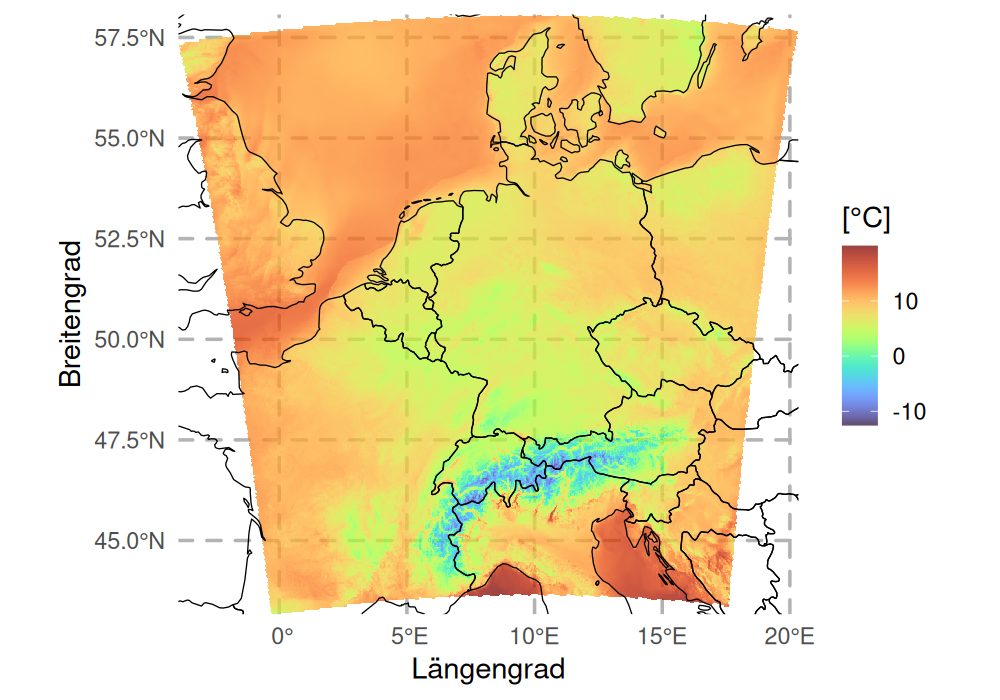
\includegraphics[width=0.8\linewidth]{figs/icon_region_Rplot.png}
\caption{Modellgebiet ICON-D2-EPS auf einem regulären Lat/Lon-Gitter dargestellt. Abgebildet ist die 0h (instant) 2-m-Temperatur Vorhersage des 1. Ensemblemitglieds vom 3.11.2025 06:00 UTC.}
\label{fig:icon}
\end{figure}

\section{Verifikationsdaten: HOSTRADA} \label{sec:host}
HOSTRADA ist ein Akronym für hochaufgelösten stündlichen Rasterdatensatz \parencite{krahenmann_high-resolution_2018,dwd_hostrada_beschreibung}. Es handelt sich um einen Referenzdatensatz für Deutschland des DWD, der seit 1995 stündlich meteorologische Parameter in der Lambert-Conformal-Conic-Projektion (LCC, EPSG:3034) mit einer horizontalen Auflösung von $1\times1\ \mathrm{km^2}$ bereitstellt. Die Daten ergeben sich aus der Interpolation von Stationsdaten unter Einbezug von Satelliten- und Modelldaten. $720 \times 938 = 333404$ Gitterpunkte sind mit Werten belegt. Das Modellgebiet ist in Abbildung \ref{fig:hostrada} dargestellt.

Die HOSTRADA 2-m-Temperaturdaten stammen genau wie die ICON-\-Modell\-gitter\-be\-schreibung aus dem Open-Data-Angebot des Deutschen Wetterdienstes und sind über
\begin{quote}
    \url{https://opendata.dwd.de/climate_environment/CDC/grids_germany/hourly/hostrada/air_temperature_mean/}
\end{quote}
abrufbar. Eine Datei umfasst die stündlichen 2-m-Temperatur Beobachtungen eines Monats im NetCDF Format.

\begin{figure}[h!]
\centering
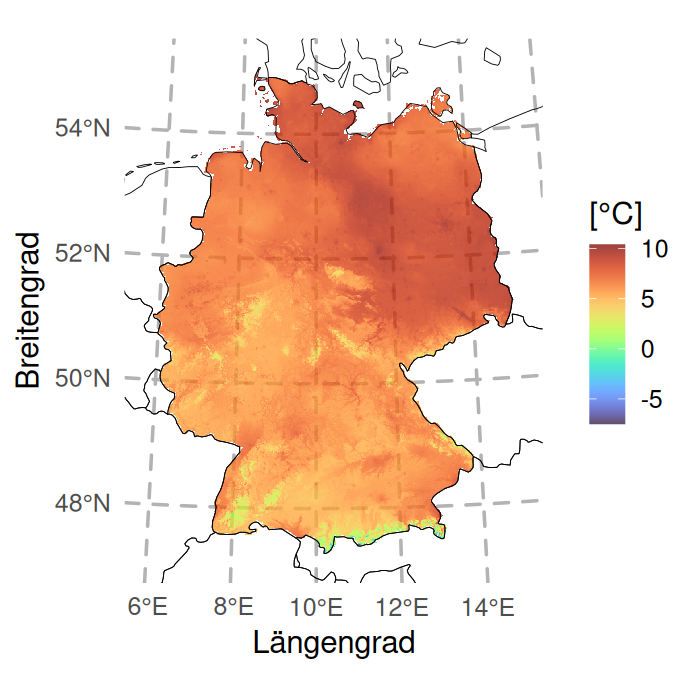
\includegraphics[width=0.55\linewidth]{figs/host_region_Rplot.png}
\caption{Modellgebiet HOSTRADA in EPSG:3034. Dargestellt ist die 2-m-Temperatur vom 3.11.2025 06:00 UTC.}
\label{fig:hostrada}
\end{figure}

\section{Projektion auf ein gemeinsames Gitter}\label{sec:proj}
Eine Besonderheit der ICON-Wettervorhersagemodelle ist das verwendete Gittersystem. Das Gitter des ICON-D2-EPS basiert auf einem unstrukturierten Dreiecksgitter in geografischen Koordinaten. Das Kürzel ICO im Modellnamen steht für \emph{ikosaedral}: Ein Ikosaeder ist ein zwanzigseitiges Polyeder. Dieses auf eine Kugel projiziert bildet die Grundlage des ICON Gitters. Die konkrete Gitterauflösung entsteht durch eine initiale Unterteilung in $n$ Root-Division-Schritte (R$n$) sowie anschließende $k$ Bisektionsschritte (B$k$), woraus ein R$n$B$k$-Gitter resultiert \parencite[Figure 2.1-2.3]{reinert2025icon_dwd}.

Im Gegensatz dazu liegen die HOSTRADA-Daten im projizierten Koordinatenreferenzsystem ETRS89 / LCC Europe (EPSG:3034) vor \parencite{dwd_hostrada_beschreibung}. Dieses basiert auf der Lambert-Conformal-Conic Projektion und ist für den europäischen Raum parametrisiert, sodass die Verzerrungen innerhalb Europas gering bleiben \parencite{map}. Vereinfacht wird bei der Projektion die Erdoberfläche zunächst auf einen Kegel abgebildet und anschließend in ein kartesisches Koordinatensystem überführt. Zudem ist das HOSTRADA feiner aufgelöst als das ICON-D2-EPS Gitter. Diesen Unterschied soll Abbildung \ref{fig:comparision} verdeutlichen.
\begin{figure}[h!]
\centering
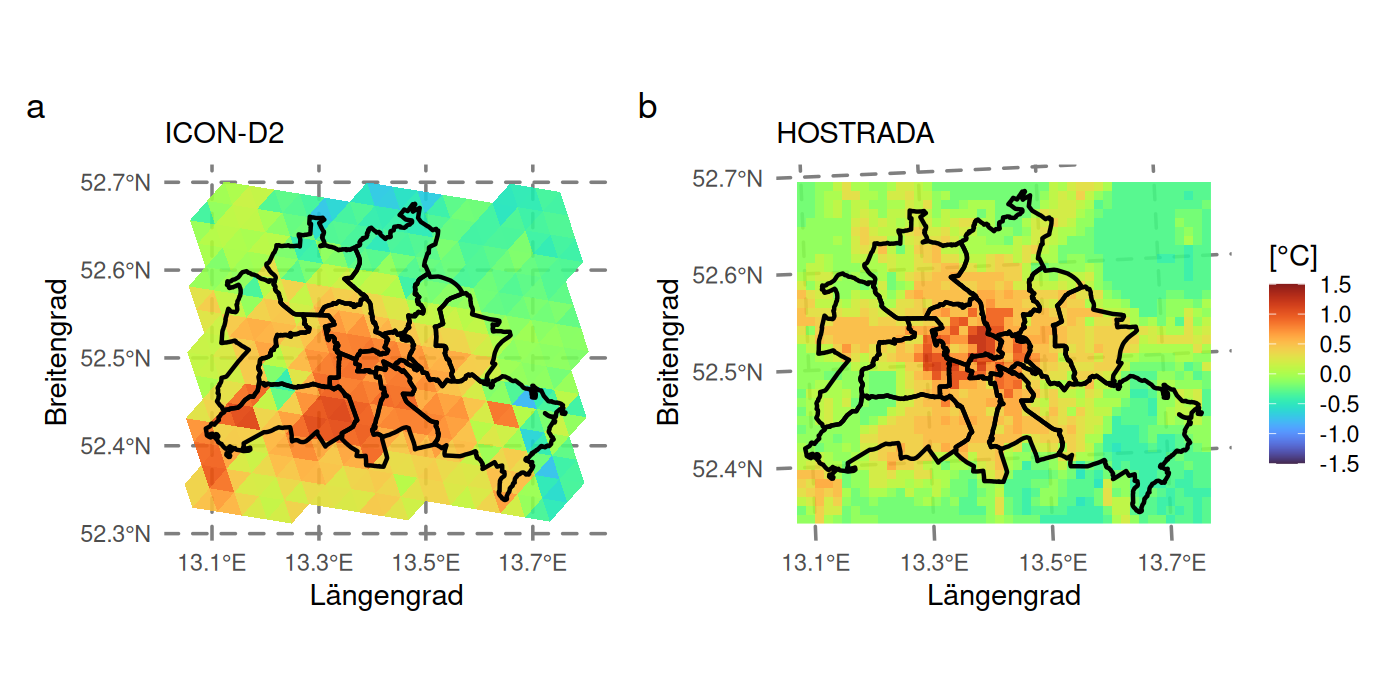
\includegraphics[width=\linewidth]{figs/proj_diff_Rplot.png}
\caption{ICON-D2-EPS Dreiecksgitter (a) im Vergleich zum HOSTRADA Raster (b) auf den Bereich Berlin eingegrenzt. Abgebildet ist die +24-h Vorhersage der 2-m-Temperatur des ersten Ensemblemitglieds zum 26.11.2025 00:00 UTC (a) und entsprechend die Temperatur vom 26.11.2025 00:00-UTC (b).}
\label{fig:comparision}
\end{figure}

Für einen Vergleich zwischen Modellvorhersagen und Beobachtungsdaten ist daher zunächst eine Überführung der beiden Modelle auf ein gemeinsames Koordinatensystem erforderlich. Wir projizieren hier die ICON-Daten auf das HOSTRADA-Gitter, das damit als Referenz für die Bewertung der Modellvorhersagen dient. Die Projektion auf das höher aufgelöste HOSTRADA-Gitter entspricht einem runterskalieren der Modellvorhersagen: Zwar werden die Modellfelder auf einer höheren räumlichen Auflösung dargestellt, der Informationsgehalt der Vorhersagen bleibt jedoch unverändert.

Ein wesentlicher praktischer Vorteil dieses Vorgehens besteht darin, dass das HOST\-RADA-Gitter von gängigen geostatistischen R-Paketen direkt verarbeitet werden kann, während das unstrukturierte Dreiecksgitter von ICON häufig nicht unterstützt wird.

Zur Änderung der Gitterprojektion empfiehlt der DWD die Nutzung des Kommandozeilenprogramms Climate Data Operators (CDO) \parencite{umwandlung}. CDO ist ein vom Max-Planck-Institut für Meteorologie entwickeltes Kommandozeilenprogramm zur Manipulation und Analyse von Klimadaten \parencite{CDO}. Für unstrukturierte Gitter wie das des ICON unterstützt CDO ausschließlich die Nearest-Neighbor-Interpolation. %Dies entspricht jedoch nicht dem Standardvorgehen des DWD, der abhängig von der jeweiligen Variable unterschiedliche Interpolationsverfahren einsetzt. So wird beispielsweise die 2-m-Temperatur mittels baryzentrischer Interpolation auf das Zielgitter übertragen \parencite{reinert2025icon_dwd}.

Nach der Projektion liegen somit sowohl die ICON-Vorhersagen als auch die HOST\-RADA-Beobachtungs\-daten auf dem gleichen räumlichen Gitter vor und können im weiteren Verlauf direkt miteinander verglichen und bewertet werden.


\section{Auswahl eines Datenausschnitts} \label{sec:used_data}
Für die Evaluation stehen mit den projizierten ICON-D2- und HOSTRADA-Daten umfangreiche, räumlich hochaufgelöste Daten für ganz Deutschland und verschiedene Zeiträume zur Verfügung. Für das das ICON-D2 existieren zudem verschiedene Vorhersagedurchläufe und Vorhersagehorizonte. Dadurch ergeben sich zahlreiche Möglichkeiten, Daten für eine Evaluation zusammenzustellen. Gegenstand der vorliegenden Arbeit sind Evaluationsmethoden probabilistischer Vorhersagen. Um diese gezielt zu untersuchen, grenzen wir die Daten ein, um eine überschaubare und nachvollziehbare Datengrundlage zu schaffen. Gleichzeitig soll die Auswahl realistische Bedingungen abbilden und nicht auf einen vollständig kontrollierten Anwendungsfall beschränkt sein. Wir schränken die Datenmenge hinsichtlich des betrachteten Zeitraums, des Vorhersagegebiets, des Vorhersagedurchlaufs und der Vorhersagehorizonte ein.

Als Evaluationszeitraum betrachten wir den November 2025. Die Beschränkung auf einen Monat ermöglicht eine überschaubare Auswertung.  Neben Evaluationsdaten verwenden wir unter anderem statistisches Postprocessing, um aus den rohen Ensemblevorhersagen des DWD probabilistische Vorhersagen zu erstellen. Dazu bedarf es Trainingsdaten, üblich ist hierbei ein Trainingsfenster von 20 bis 40 Tagen \parencite{gneiting2014calibration}, sodass Vorhersage und Verifikationsdaten des Oktobers 2025 ebenfalls als Daten einfließen.

Das Untersuchungsgebiet wird auf eine Region um Berlin eingegrenzt. Die Wahl der Region erfolgte in Abstimmung mit dem Betreuer sowohl aufgrund eines persönlichen Bezugs zur Region als auch aufgrund ihrer hohen Bevölkerungsdichte und der damit verbundenen gesellschaftlichen Relevanz. Als Grundlage für die probabilistischen Vorhersagen dienen die stündlichen Ensemblevorhersagen des ICON-D2-EPS. Dabei betrachten wir jeweils den um 00:00 UTC initialisierten Modelllauf. Dies stellt eine einfache und nachvollziehbare Auswahl des Modelllaufs dar, weil dieser der erste verfügbare Modelllauf des jeweiligen Tages ist. Analysiert werden die Vorhersagehorizonte von 24 und 48 Stunden. Die beiden Horizonte wählen wir, weil zwischen ihnen 24 Stunden liegen und wir somit für beide Horizonte dieselben Beobachtungsdaten des Novembers verwenden können. Dadurch lassen sich die Vorhersagehorizonte direkt miteinander vergleichen.

Der Auswahl der Daten entsprechend sind die Ergebnisse also als exemplarische Untersuchung probabilistischer Vorhersagen zu verstehen und nicht als vollständige oder repräsentative Evaluation der Vorhersagequalität des ICON-D2-EPS.


\section{Vorbereitung der Daten} 
Die Vorbereitung der Vorhersagedaten folgende Schritte: Mithilfe des CDO-Befehls \texttt{gennn} wurden zunächst Interpolationsgewichte auf Basis der Gitterbeschreibungen von HOSTRADA und ICON-D2-EPS erzeugt und als NetCDF-Datei gespeichert. Anschließend wurden über das Webinterface von PAMORE die ICON-D2-EPS-Daten für den Zeitraum vom 1. Oktober 2025 bis zum 30. November 2025 jeweils täglich um 00:00 UTC mit Vorhersagehorizonten von 24 und 48 Stunden abgefragt. Die Daten wurden anschließend über den FTP-Server heruntergeladen und gespeichert. Mithilfe der zuvor erzeugten Interpolationsgewichte wurden die ICON-D2-EPS Daten für jeden Vorhersagehorizont mit dem CDO-Befehl \texttt{remap} auf das HOSTRADA-Gitter projiziert. Abschließend wurden die Ensemblemitglieder je Vorhersagehorizont und Tag zu einer gemeinsamen Datei zusammengeführt und als NetCDF-Datei gespeichert. Dieser gesamte Prozess wurde mithilfe eines Python Skripts teilweise automatisiert. Die HOSTRADA-Daten mussten nicht weiter vorverarbeitet werden.

\section{Zusammenfassung und Indizierung} \label{sec:indx}

Zusammenfassend vergleichen wir probabilistische Vorhersagen, die aus den auf das HOSTRADA-Gitter projizierten Ensemblemitgliedern des ICON-D2-EPS des jeweils um 00:00 UTC initialisierten Modelllaufs abgeleitet werden, mit den entsprechenden Temperaturbeobachtungen des HOSTRADA. Der Untersuchungszeitraum umfasst den November 2025 und damit insgesamt 30 Tage vom 01.11.2025, 00:00 UTC, bis zum 30.11.2025, 00:00 UTC. Analysiert werden Vorhersagehorizonte von 24 und 48 Stunden für ein Vorhersagegebiet um Berlin, das insgesamt $38 \times 46 = 1748$ Gitterzellen umfasst.

Zur einheitlichen Beschreibung der Verifikationsdaten führen wir folgende Indizierung ein: Es bezeichne $t \in T = \{1,\dots,30\}$ den Verifikationstag im November 2025, \mbox{$l \in L = \{1,\dots,1748\}$} die jeweilige Gitterzelle, $m \in M = \{1,\dots,20\}$ das Ensemblemitglied des ICON-D2-EPS sowie $h \in H = \{24\h, 48\h\}$ den betrachteten Vorhersagehorizont. 

Wir schreiben also $y_{l}^{(t)}$ für die beobachtete HOSTRADA Temperatur zum Zeitpunkt 00:00 UTC am Verifikationstag $t$ in der Gitterzelle $l$. Entsprechend schreiben wir  $x_{l,h,m}^{(t)}$ für die Punktvorhersage für 00:00 UTC zum Verifikationstag $t$ an Gitterzelle $l$, erzeugt vom $m$-ten Ensemblemitglied zum Vorhersagehorizont $h$. Initialisiert ist diese Vorhersage entweder einen Tag ($h=24\h$) oder zwei Tage ($h=48\h$) vor dem Verifikationstag. Die Temperatur geben wir in Grad Celsius an. Zur Veranschaulichung der Struktur und Beschaffenheit der Verifikationsdaten betrachten wir exemplarisch den Vorhersagehorizont $h=24\h$. Tabelle \ref{tab:datensatz} zeigt hierzu einen beispielhaften Datenausschnitt, während Abbildung \ref{fig:daten_schema} die Daten schematisch darstellt.

\begin{table}[ht]
    \centering
    \fontsize{10.5}{12}\selectfont
    \newcolumntype{C}{>{\centering\arraybackslash}X}
    \newcolumntype{Y}{>{\centering\arraybackslash}p{2cm}}
    \caption{Ausschnitt zum Aufbau des Verifikationsdatensatzes zum Vorhersagehorizont $24\h$.}
    \label{tab:datensatz}
    \begin{tabularx}{\textwidth}{Y C C C C C C C C}
        \toprule
        Datum & $t$ & $l$ & $y_{l}^{(t)}$ & $x_{l,24\h,1}^{(t)}$ & $x_{l,24\h,2}^{(t)}$ & $x_{l,24\h,3}^{(t)}$ & $\dots$ & $x_{l,24\h,20}^{(t)}$ \\
        \midrule
        2025110100 & 1 & 1 & 7.3 & 7.5 & 7.9 & 6.2 & $\dots$ & 7.5 \\
        2025110100 & 1 & 2 & 7.3 & 7.4 & 7.9 & 6.3 & $\dots$ & 7.4 \\
        2025110100 & 1 & 3 & 7.3 & 7.5 & 8.0 & 6.5 & $\dots$ & 7.4 \\
        2025110100 & 1 & 4 & 7.4 & 7.5 & 8.0 & 6.5 & $\dots$ & 7.4 \\
        2025110100 & 1 & 5 & 7.7 & 7.7 & 8.2 & 6.8 & $\dots$ & 7.6 \\
        $\vdots$ & $\vdots$ & $\vdots$ & $\vdots$ & $\vdots$ & $\vdots$ & $\vdots$ & $\vdots$ & $\vdots$ \\
        2025113000 & 30 & 1744 & 4.7 & 2.7 & 4.1 & 2.7 & $\dots$ & 4.8 \\
        2025113000 & 30 & 1745 & 4.7 & 2.5 & 4.0 & 2.6 & $\dots$ & 4.7 \\
        2025113000 & 30 & 1746 & 4.7 & 2.4 & 3.7 & 2.3 & $\dots$ & 4.7 \\
        2025113000 & 30 & 1747 & 4.7 & 2.4 & 3.7 & 2.3 & $\dots$ & 4.7 \\
        2025113000 & 30 & 1748 & 4.7 & 2.2 & 3.5 & 2.2 & $\dots$ & 4.8 \\
        \bottomrule
    \end{tabularx}
\end{table}


\begin{figure}[h] 
\centering
\resizebox{.85\textwidth}{!}{
\begin{tikzpicture}%[scale=0.5,, transform shape]
\def\N{4}
\def\dy{-6.5} % vertikaler Versatz der Verifikationszeile nach unten
\def\dx{7} %horizontaler versatz der gitter

% =========================================================
% Zeilenbeschriftung links: Ensemble-Reihe
% =========================================================
\node[rotate=90] at (-1.4,2.3) {Regridded ICON-D2-EPS};
% =========================================================
% ENSEMBLE-REIHE (oben)
% =========================================================
% --- Ensemble-Grafik 1 ---
\begin{scope}[shift={(0,0)}]
% Ensemble 3 (hinten)
\begin{scope}[shift={(-0.8,0.6)}]
    \fill[purple!10] (0,0) rectangle (\N,\N);
    \draw[purple!70, opacity=0.5] (0,0) grid (\N,\N);
\end{scope}
% Ensemble 2 (mittig)
\begin{scope}[shift={(-0.4,0.3)}]
    \fill[teal!10] (0,0) rectangle (\N,\N);
    \draw[teal!70, opacity=0.7] (0,0) grid (\N,\N);
\end{scope}
% Ensemble 1 (vorne)
\fill[blue!10] (0,0) rectangle (\N,\N);
\draw[blue!70, thick] (0,0) grid (\N,\N);


% Werte
\node  at (0.5,\N-0.5) { \scalebox{0.7}[1]{$x_{1,h,1}^{(1)}$}};
\node[font=\small] at (\N-0.5,0.5) {\scalebox{0.77}[1]{$x_{1748,h,1}^{(30)}$}};
% rechts daneben
\node[font=\tiny] at (1.5,\N-0.5) {$\cdots$};
% darunter
\node[font=\tiny] at (0.5,\N-1.5) {$\vdots$};
% links neben B
\node[font=\tiny] at (\N-1.5,0.5) {$\cdots$};
% oberhalb von B
\node[font=\tiny] at (\N-0.5,1.5) {$\vdots$};


% Klammer
\draw[decorate, decoration={brace, amplitude=13pt}]
(-0.7,\N+.7) -- (0.15,\N+.1)
node[near end, yshift=20pt,xshift=35pt,font=\small]
{Ensemble $1, \ldots, 20$};
\node at (1.6,-0.7) {Initialzeit: 31.10.2025 00:00 UTC};
\end{scope}

\node at (5,2) {\Large $\cdots$};

% --- Ensemble-Grafik 2 ---
\begin{scope}[shift={(\dx,0)}]
\begin{scope}[shift={(-0.8,0.6)}]
    \fill[purple!10] (0,0) rectangle (\N,\N);
    \draw[purple!70, opacity=0.5] (0,0) grid (\N,\N);
\end{scope}
\begin{scope}[shift={(-0.4,0.3)}]
    \fill[teal!10] (0,0) rectangle (\N,\N);
    \draw[teal!70, opacity=0.7] (0,0) grid (\N,\N);
\end{scope}
\fill[blue!10] (0,0) rectangle (\N,\N);
\draw[blue!70, thick] (0,0) grid (\N,\N);
\node at (1.6,-0.7) {Initialzeit: 29.11.2025 00:00 UTC};


\node  at (0.5,\N-0.5) { \scalebox{0.7}[1]{$x_{1,h,1}^{(30)}$}};
\node[font=\small] at (\N-0.5,0.5) {\scalebox{0.77}[1]{$x_{1748,h,1}^{(30)}$}};
% rechts daneben
\node[font=\tiny] at (1.5,\N-0.5) {$\cdots$};
% darunter
\node[font=\tiny] at (0.5,\N-1.5) {$\vdots$};
% links neben B
\node[font=\tiny] at (\N-1.5,0.5) {$\cdots$};
% oberhalb von B
\node[font=\tiny] at (\N-0.5,1.5) {$\vdots$};
\end{scope}

% =========================================================
% Pfeil: Vorhersagehorizont (nach unten, innerhalb der Spalte)
% =========================================================
\draw[->, thick]
    (2,-1.3) -- node[right, align=left] {Horizont\\ +24 h} (2,\dy+\N+0.3);
\draw[->, thick]
    (2+\dx,-1.3) -- node[right, align=left] {Horizont\\ +24 h} (2+\dx,\dy+\N+0.3);
% =========================================================
% Zeilenbeschriftung links: Verifikations-Reihe
% =========================================================
\node[rotate=90] at (-1.4,\dy+2) {HOSTRADA};

% =========================================================
% VERIFIKATIONS-REIHE (unten)
% =========================================================
\begin{scope}[shift={(0,\dy)}]
\draw[black, thick] (0,0) grid (\N,\N);
\node at (2,-0.7) {01.11.2025 00:00 UTC};

\node  at (0.5,\N-0.5) { \scalebox{0.8}[1]{$y_{1}^{(1)}$}};
\node at (\N-0.5,0.5) {\scalebox{0.8}[1]{$y_{1748}^{(1)}$}};
\node[font=\tiny] at (1.5,\N-0.5) {$\cdots$};
\node[font=\tiny] at (0.5,\N-1.5) {$\vdots$};
\node[font=\tiny] at (\N-1.5,0.5) {$\cdots$};
\node[font=\tiny] at (\N-0.5,1.5) {$\vdots$};

\end{scope}

\node at (5,\dy+2) {\Large $\cdots$};


\begin{scope}[shift={(7,\dy)}]
\draw[black, thick] (0,0) grid (\N,\N);
\node at (2,-0.7) {30.11.2025 00:00 UTC};
\node  at (0.5,\N-0.5) { \scalebox{0.8}[1]{$y_{1}^{(30)}$}};
\node at (\N-0.5,0.5) {\scalebox{0.8}[1]{$y_{1748}^{(30)}$}};
\node[font=\tiny] at (1.5,\N-0.5) {$\cdots$};
\node[font=\tiny] at (0.5,\N-1.5) {$\vdots$};
\node[font=\tiny] at (\N-1.5,0.5) {$\cdots$};
\node[font=\tiny] at (\N-0.5,1.5) {$\vdots$};
\end{scope}

\end{tikzpicture}
}
\caption{Schematische Darstellung der Verifikationsdatenpaare zum Vorhersagehorizont $h=24\h$.}
\label{fig:daten_schema}
\end{figure}

\FloatBarrier
\section{Deskription der Daten} \label{sec:desc}
\subsection{HOSTRADA Temperaturbeobachtungen November 2025}
Wir betrachten zunächst die zeitlichen und anschließend die räumlichen Aspekte der Temperaturbeobachtungen anhand visueller Darstellungen. Abbildung \ref{fig:nov_temp} zeigt die zeitliche Entwicklung und Häufigkeitsverteilung der Temperaturen Berlins für den November 2025, 00:00 UTC der HOSTRADA-Verifikationsdaten. Die zeitliche Entwicklung der Temperaturen beginnt mit einer Abkühlung vom Monatsbeginn bis zum letzten Monatsdrittel. Die niedrigsten Temperaturen werden zwischen dem 21. und 24. November erreicht. Anschließend steigen die Temperaturen zum Monatsende wieder leicht an. Zudem ist erkennbar, dass die Gesamtvariabilität der Temperaturbeobachtungen überwiegend auf zeitlichen Unterschieden zwischen den Tagen beruht. Innerhalb eines Tages ist die Variation oft gering.

\begin{figure}[h]
    \centering
    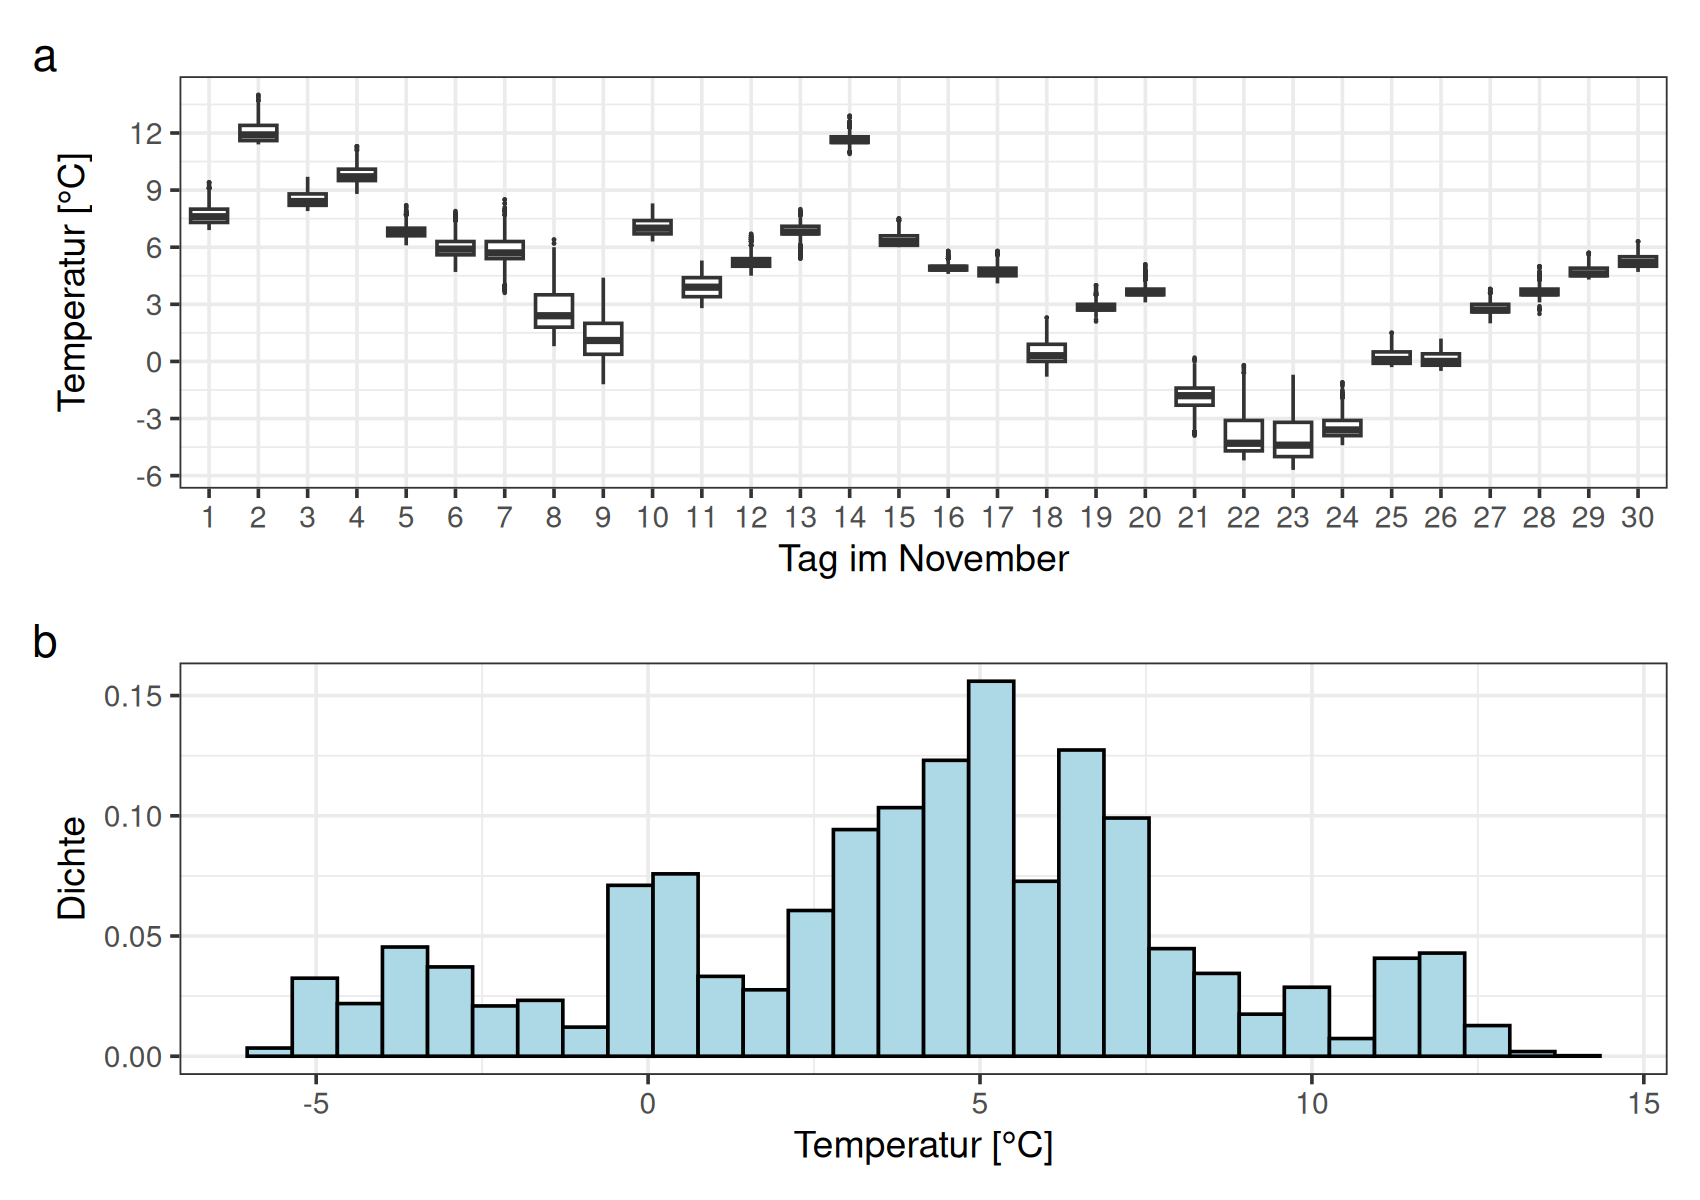
\includegraphics[width=0.9\linewidth]{figs/nov_desc.png}
    \caption{HOSTRADA: Temperatur in Berlin im November 2025, 00:00 UTC. Boxplots der Temperaturverteilung pro Tag über alle Gitterzellen (a) und Histogramm der beobachteten Temperaturen über alle Tage und Gitterzellen (b).}
    \label{fig:nov_temp}
\end{figure}

Die Häufigkeitsverteilung weißt einen Schwerpunkt zwischen etwa $4\C$ und $6\C$ auf. Temperaturen unter dem Gefrierpunkt sowie Werte oberhalb von $10\C$ treten selten auf. Die Verteilung ist asymmetrisch, ungleichmäßig und es zeigen sich mehrere lokale Häufigkeitsmaxima. Diese spiegeln sowohl die milde Witterung zu Monatsbeginn als auch die Kältephase vom 21. bis 24. wider.

Abbildung \ref{fig:nov_temp_spat} zeigt die räumliche Verteilung der mittleren Temperatur im November 2025 um  00:00 UTC über das Untersuchungsgebiet.
Dabei wird  ein Stadt-Land-Gradient deutlich: Die höchsten Temperaturen werden im Innenstadtbereich Berlins erreicht und an den Randgebieten nehmen die Temperaturen kontinuierlich ab. Besonders die südöstlichen und nordöstlichen Stadtränder weisen vergleichsweise niedrige Temperaturen auf. Dieses räumliche Muster entspricht einem Urban-Heat-Island-Effekt, der im HOSTRADA explizit modelliert wird und daher erwartungsgemäß erkennbar ist \parencite{krahenmann_high-resolution_2018}.

Ergänzend dazu können wir ausgewählte räumliche Eigenschaften des Untersuchungsgebiets genauer betrachten. Dazu ist in Abbildung \ref{fig:berlin_spat} die Verteilung von Gewässern, Wald- und Ackerflächen im untersuchten Gebiet dargestellt. Anhand dieser Abbildung wird deutlich, dass in der HOSTRADA Temperaturkarte (vgl. Abbildung \ref{fig:nov_temp_spat}) Wälder und Ackerflächen geringere mittlere Temperaturen als andere Bereiche aufweisen. Gewässer fallen hingegen nicht besonders auf.

\begin{figure}[h]
    \centering
    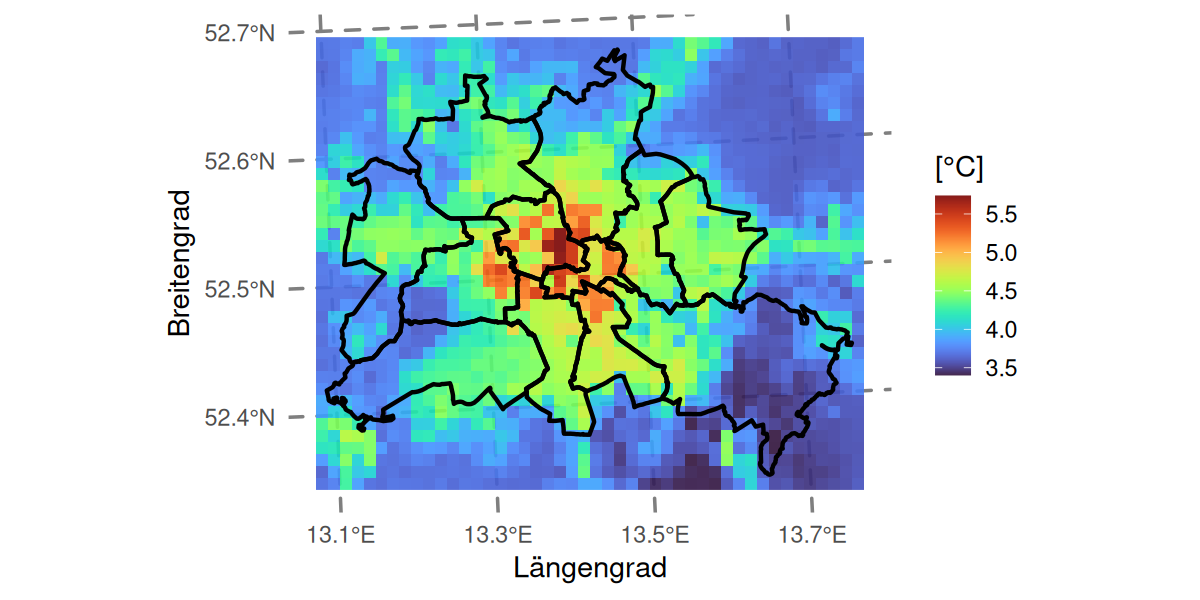
\includegraphics[width=\linewidth]{figs/nov_spat_Rplot.png}
    \caption{HOSTRADA: Mittlere Temperatur in Berlin im November 2025, 00:00 UTC pro Gitterzelle.}
    \label{fig:nov_temp_spat}
\end{figure}



\begin{figure}[h]
    \centering
    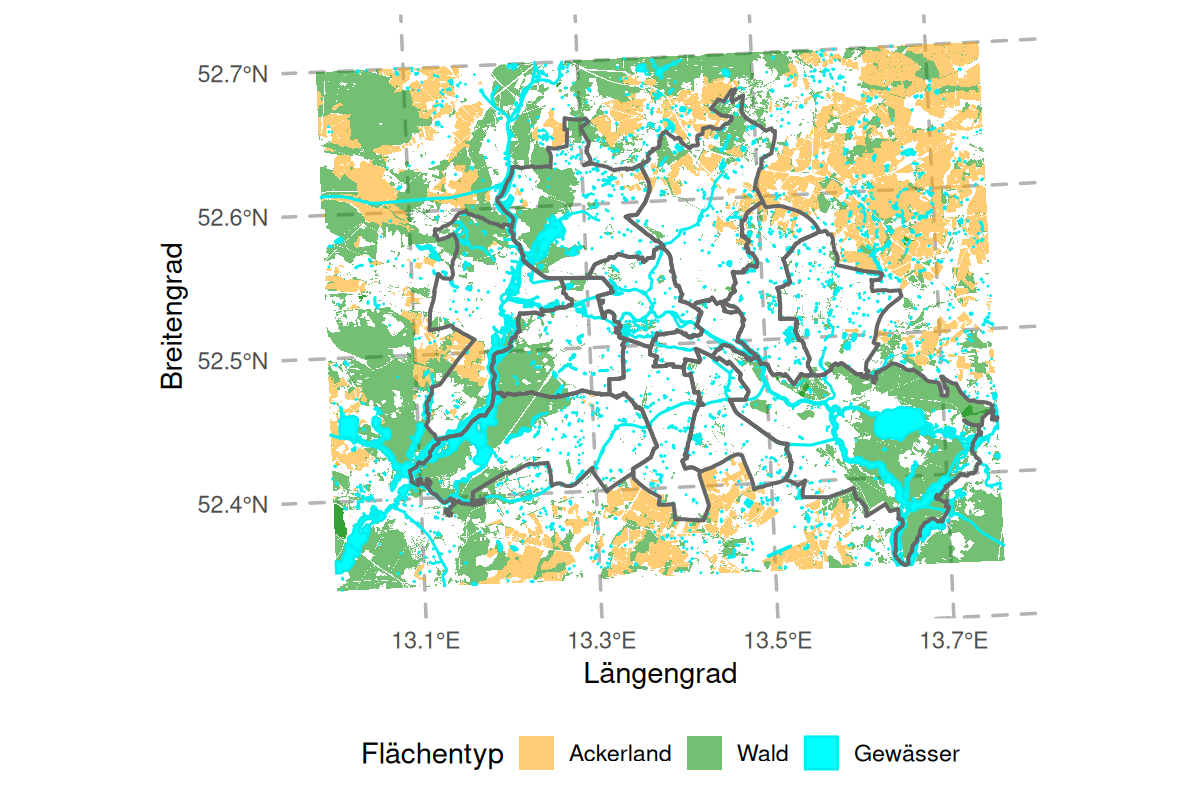
\includegraphics[width=.9\linewidth]{figs/berlin_geo_Rplot.png}
    \caption{Räumliche Verteilung der Gewässer, Wald- und Ackerflächen im untersuchten Gebiet.
    Datengrundlage: \href{https://download.geofabrik.de/europe/germany/brandenburg.html}{OpenStreetMap-Daten}.}
    \label{fig:berlin_spat}
\end{figure}


\FloatBarrier
\subsection{ICON-D2-EPS Temperaturvorhersagen November 2025}
Um die ICON-D2-EPS-Vorhersagen zu beschreiben, vergleichen wir sie direkt mit den HOSTRADA-Daten. Dabei betrachten wir, wie im vorherigen Abschnitt, zunächst zeitliche und anschließend räumliche Aspekte.

Abbildung \ref{fig:icon_time} zeigt die zeitliche Entwicklung der ICON-D2-Ensemblevorhersagen im Vergleich zur HOSTRADA. Insgesamt bilden die Ensemblevorhersagen den zeitlichen Temperaturverlauf der HOSTRADA-Daten gut ab. Beim höheren Vorhersagehorizont nimmt die Streuung der Ensemblemitglieder jedoch zu. Auffällig ist zudem eine tendenzielle Überschätzung der Temperaturen um den 9.11 sowie dem 22.11. Dabei zeichnet sich jedoch kein Ensemblemitglied durch eine auffallend systematisch zu hohe oder zu niedrige Temperaturvorhersage aus.

Abbildung \ref{fig:nov_temp_spat} zeigt die räumliche Verteilung der mittleren Temperaturvorhersagen über alle Ensemble getrennt nach Vorhersagehorizont. Die räumliche Struktur erscheint dabei unabhängig vom Vorhersagehorizont. Wie bei den HOSTRADA-Daten wird ein Stadt-Land-Gradient deutlich. Die Darstellung ist jedoch insgesamt glatter und im Stadtkern weniger extrem. Im Vergleich zu den HOSTRADA-Daten (Abbildung \ref{fig:nov_temp_spat}) fallen jedoch die Gewässer Teglersee (links oben), Havel (links unten) und insbesondere der Große Müggelsee (rechts unten) (vgl. Abbildung \ref{fig:berlin_spat}) durch eine höhere Temperatur als deren Umgebung auf.






\begin{figure}[h]
    \centering
    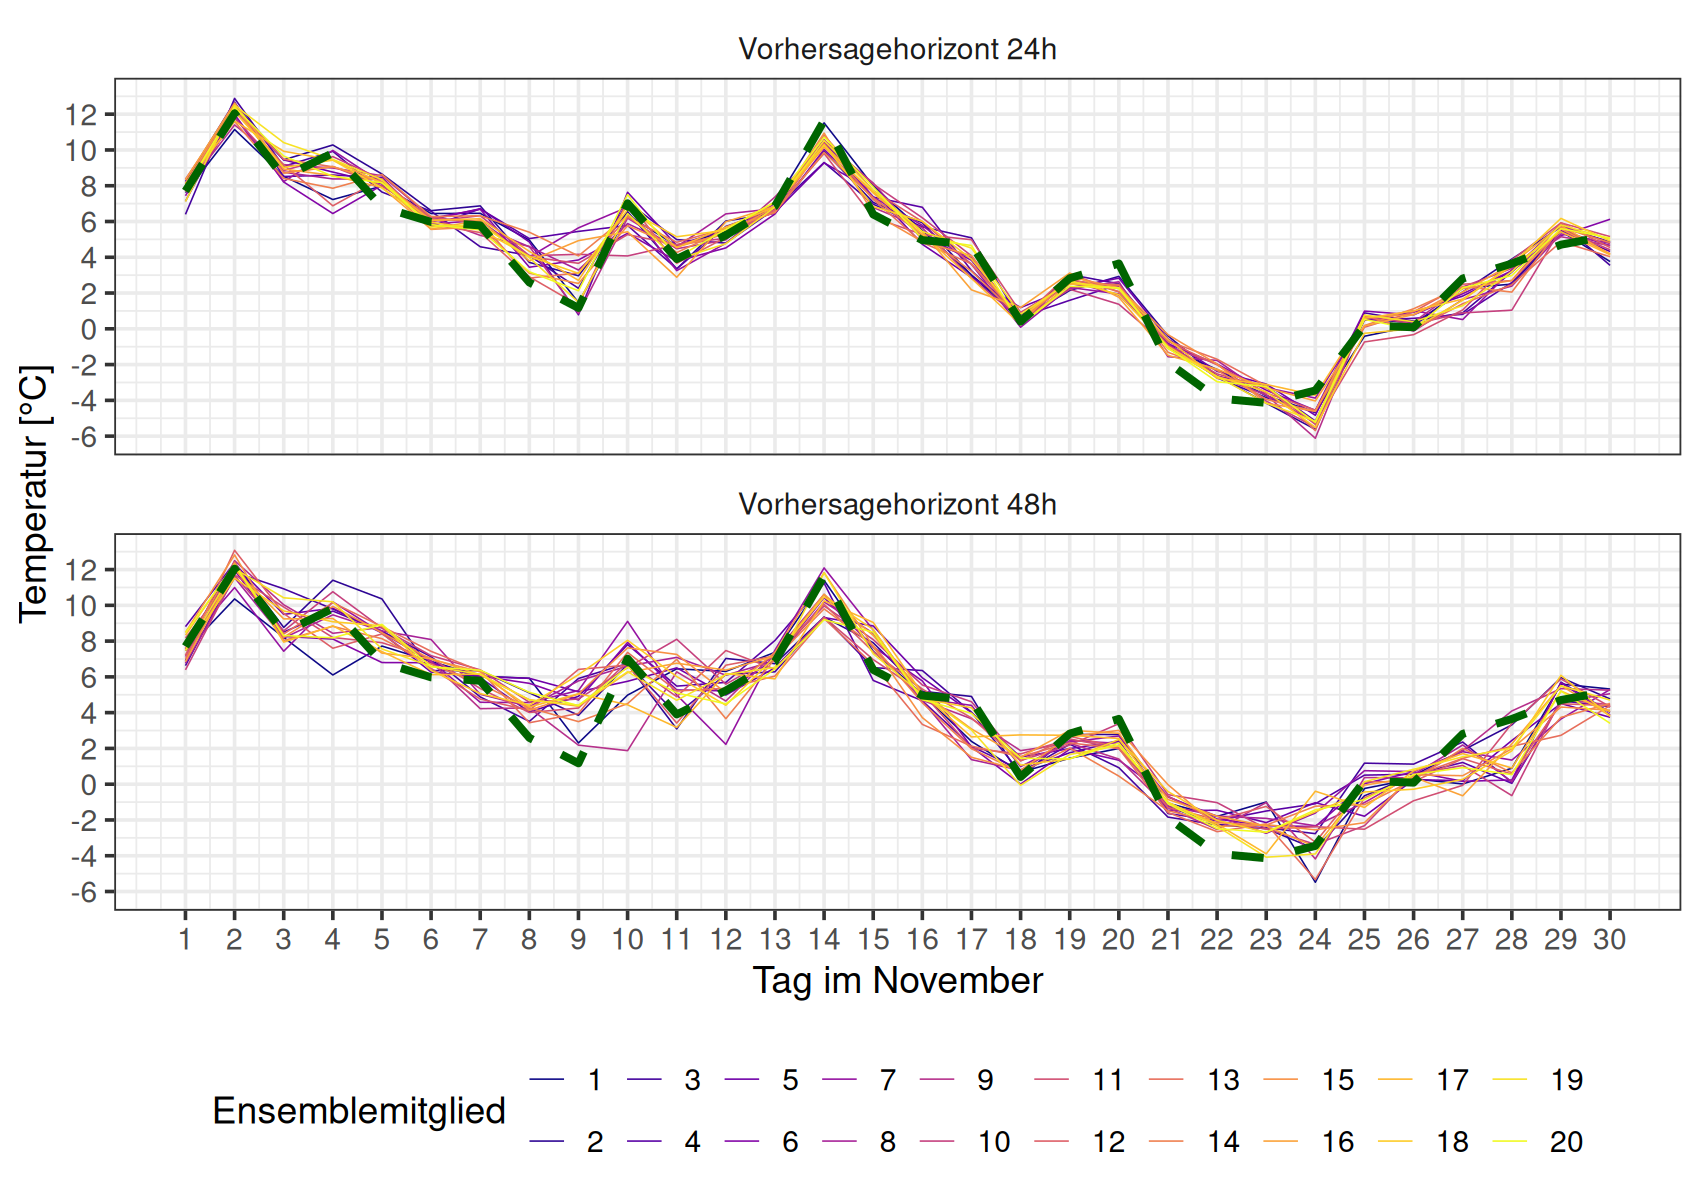
\includegraphics[width=.95\linewidth]{figs/icon_time.png}
    \caption{ICON-D2-EPS: Mittlere Temperatur in Berlin pro Tag im November 2025, 00:00 UTC pro Ensemblemitglied für beide Vorhersagehorizonte. Die gestrichelte Linie zeigt die HOSTRADA- Temperatur als Referenz.}
    \label{fig:icon_time}
\end{figure}

\begin{figure}[!ht]
    \centering
    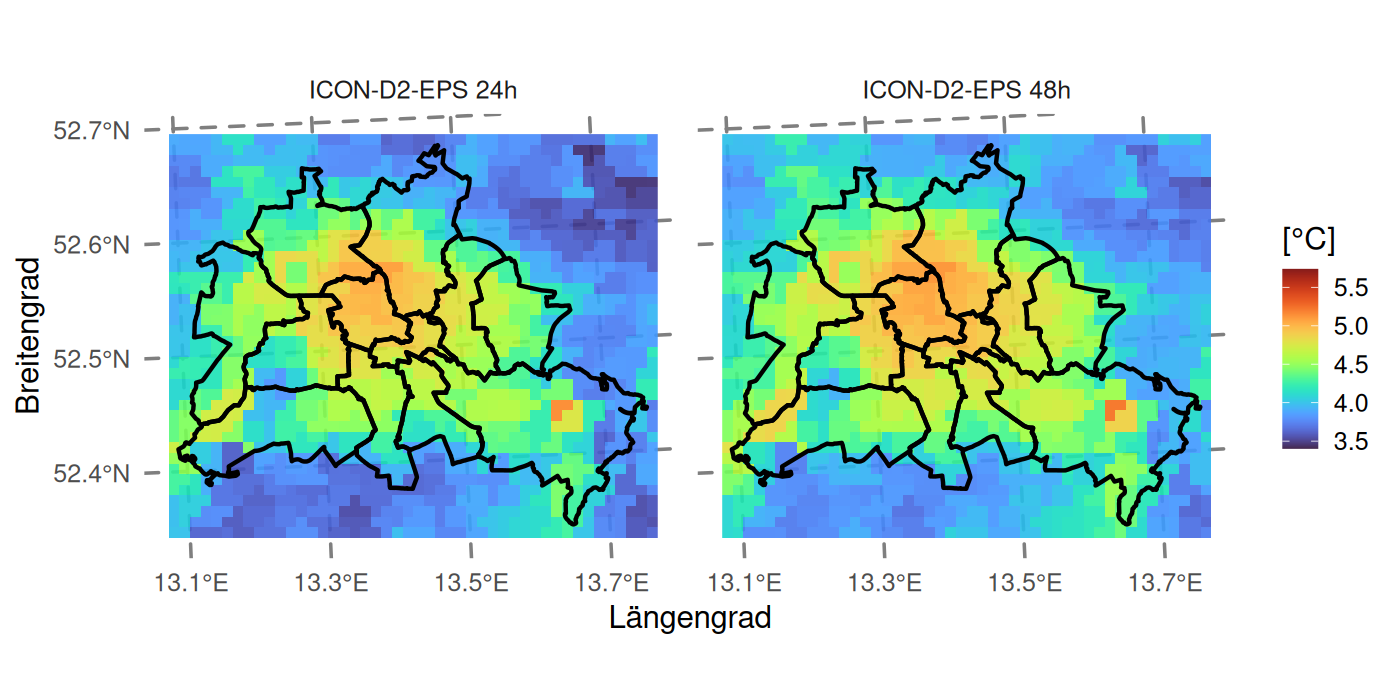
\includegraphics[width=1.02\linewidth]{figs/mean_icon_spat_Rplot.png}
    \caption{
     ICON-D2-EPS: Mittlere Temperatur in Berlin pro Gitterzelle im November 2025, 00:00 UTC getrennt nach Vorhersagehorizont, über alle Ensemblemitglieder gemittelt.}
    \label{fig:icon_temp_spat}
\end{figure}





\chapter{Vorhersagen und Evaluationsvorgehen} \label{chap:meth}
Im vorherigen Kapitel haben wir die Datengrundlage beschrieben. Für die Evaluation fehlen jedoch noch probabilistische Vorhersagen. In diesem Kapitel soll es daher vornehmlich darum gehen, wie wir auf der Basis von Ensemblevorhersagen probabilistische Vorhersagen erstellen können. Zu Beginn beschreiben wir jedoch in Abschnitt \ref{sec:sofware} die verwendete Software für die Berechnungen in der vorliegenden Arbeit. Erst dann gehen wir in den Abschnitten \ref{sec:pre_postproc} und \ref{sec:postproc} darauf ein, wie wir die probabilistischen Vorhersagen erstellen. Schließlich fassen wir in Abschnitt \ref{sec:meth_eval} die zur Evaluation erstellten Vorhersagen zusammen und erläutern kurz das Evaluationsvorgehen. Abschließend formulieren wir einige Erwartungen an die Güte der erstellten Vorhersagen.

\section{Software, Implementierung und Reproduzierbarkeit} \label{sec:sofware}
Für das Erstellen der probabilistischen Vorhersagen, die Evaluation sowie den theoretischen Teil dieser Arbeit wurden alle Analysen mit \texttt{RStudio} \parencite{Rstudio} in der Programmiersprache R \parencite{R} durchgeführt. Im Folgenden werden die wichtigsten der verwendeten Pakete vorgestellt. Zur Bearbeitung der Daten wurde das Paket \texttt{tidyverse} \parencite{tidy} verwendet. Insbesondere die darin enthaltene Bibliothek \texttt{ggplot2} \parencite{ggplot2} bildet die Grundlage für alle in dieser Arbeit erstellten Abbildungen. Für die Bearbeitung und Darstellung geografischer Daten kamen die Pakete \texttt{terra} \parencite{terra}, \texttt{tidyterra} \parencite{tidyterra} und \texttt{sf} \parencite{sf} zum Einsatz. Die Regressionen im Rahmen des Postprocessings wurden mit dem Paket \texttt{crch} \parencite{crch} durchgeführt. Zur Berechnung des Quantilscores und des CRPS kam das Paket \texttt{scoringRules} \parencite{scoringRules} zum Einsatz. Der PAV-Algorithmus wurde mit dem Paket \texttt{isotone} \parencite{isotone} berechnet. 

Für die im Rahmen der Evaluation verwendeten Methoden war kein R-Paket bekannt, das alle benötigten Funktionalitäten bereitstellt. Die Implementierung greift jedoch teilweise auf bereits vorhandenen Code zurück. So wurde der Code zur Erstellung der Reliabilitätsdiagramme auf Grundlage des ergänzenden Materials \textcite{gneiting2023supp} angepasst und unter anderem auf \texttt{ggplot2} umgestellt. In ähnlicher Weise basiert die Implementierung der Zerlegungsdiagramme auf dem Code Material von \textcite{gneiting2023model}. Für die Zerlegung des CRPS mithilfe des Quantilscores lag hingegen kein entsprechender Beispielcode vor, sodass diese Methode selbst implementiert wurde. Der vollständige Code zur Auswertung ist in einem GitHub-Repository über
\begin{quote}
    \url{https://github.com/harro-rejewski/bachelor_thesis.git}
\end{quote}
verfügbar. Zur Gewährleistung der Reproduzierbarkeit können entweder das bereitgestellte Docker-Image oder die entsprechende \texttt{.lock}-Datei verwendet werden, über die sich die verwendeten Paketversionen nachvollziehen und reproduzieren lassen.


\section{Erstellen von probabilistischen Vorhersagen}\label{sec:pre_postproc}
Gegeben seien die Ensemblevorhersagen für einen Verifikationstag, Ort und Vorhersagehorizont
\[
x_{l,h}^{(t)}=\left(x_{l,h,1}^{(t)},\dots,x_{l,h,20}^{(t)}\right).
\]
Ziel ist es, auf Basis dieser Information eine probabilistische Vorhersage zu erstellen. Formal suchen wir also eine Abbildung, die die Ensemblevorhersagen in eine Wahrscheinlichkeitsverteilung und damit in eine Vorhersage $F^{(t)}_{l,h}$ überführt\footnote{Im Sinne des Vorhersageraums \ref{def::room} entspricht dies also einem Markovkern.}, wobei $F_{l,h}^{(t)}$ die probabilistische Vorhersage für die Gitterzelle $l$, den Vorhersagehorizont $h$ und den Verifikationstag $t$ bezeichnet. Idealerweise approximiert diese Vorhersage die bedingte Verteilung, wodurch die Eigenschaft der Auto-Kalibrierung aus Abschnitt \ref{sec:auto_cal} erfüllt wäre.
\[
F^{(t)}_{l,h}(y) \approx \mathbb{P}(Y^{(t)}_{l}\le y \mid X_{l,h}^{(t)}=x^{(t)}_{l,h})\,,
\]
wobei $X_{l,h}^{(t)}$ die Zufallsvariable der Ensemblevorhersagen, und  $Y^{(t)}_{l}$ die der Temperaturbeobachtung zugrundeliegende Zufallsvariable bezeichnen. Wir fassen also sowohl die Ensemblevorhersagen $x_{l,h}^{(t)}$ als auch die Temperaturbeobachtung $y^{(t)}_{l}$ als Realisationen von Zufallsvariablen auf. 

Die einfachste probabilistische Vorhersage, die wir nun erstellen können, ist die empirische Verteilung der Ensemblemitglieder. Dem Ensemble ordnen wir also die Verteilungsfunktion
\[
F_{l,h}^{(\mathrm{emp},t)}(y)= \frac{1}{20}\sum_{m=1}^{20} \mathds{1}\!\left\{x_{l,h,m}^{(t)}\le y\right\}
\]
zu. Wir nennen diese Vorhersage die \emph{empirische Vorhersage}.


\section{Statistisches Postprocessing}\label{sec:postproc}
Ensemblevorhersagen weisen häufig systematische Fehler in Form von Bias und Dispersionsfehlern auf \parencite{vannitsem_statistical_2021}. Dispersionsfehler äußern sich meist in einer zu geringen Streuung der Ensemblemitglieder. Aufgrund dieser möglichen Fehler ist es sinnvoll, Ensemblevorhersagen mithilfe statistischer Postprocessing Verfahren nachzubearbeiten und nicht direkt die empirische Verteilung dieser als Vorhersage zu verwenden \parencite{vannitsem_statistical_2021, gneiting2014probabilistic}.

Die Variante des Postprocessings, die wir anwenden, ist ein univariater Ansatz. Dabei erhalten wir für jede Kombination aus Gitterzelle und Vorhersagehorizont eine separate Vorhersage \parencite{climaguidelines}. Räumliche und zeitliche Abhängigkeiten bleiben somit nur durch die Ensemblesvorhersagen erhalten und werden im Postprocessing nicht explizit modelliert. Dies steht im Gegensatz zu Ansätzen, bei denen ein gemeinsames multivariates Modell über mehrere Orte oder Zeitpunkte spezifiziert wird \parencite{vannitsem_statistical_2021}.

Konkret nutzten wir hier  \emph{Ensemble Model Output Statistics} (EMOS). Hierbei handelt es sich, um eine verbreitete univariate Postprocessing-Methode \parencite{gneiting2005emos,gebetsberger2018estimation}. Dabei dienen die Ensemblemitglieder als Kovariaten einer verteilungsbasierten parametrischen Regression, deren Parameter mithilfe von Trainingsdaten geschätzt werden. Seinen dazu vereinfacht ohne Zelle und Horizont  $x_1,\dotsc,x_M$ Ensemblevorhersagen und $Y$ der Vorhersagegegenstand und $f$ eine zu spezifizierende parametrische Wahrscheinlichkeitsverteilung. Dann lautet das allgemeine EMOS Modell
\[
Y \mid x_1,\dotsc,x_M \sim f(\,\cdot \mid x_1,\dotsc,x_M\,).
\]

Betrachten wir die Temperatur als Response, so wird diese im Rahmen von EMOS häufig durch eine Normalverteilung modelliert, wobei die Ensemblemitglieder als austauschbar gelten \parencite{gneiting2014probabilistic}. In diesem Fall entspricht EMOS einer heteroskedastischen Gaußschen Regression.  Das Modell lautet
\begin{equation} \label{eq:emos}
\begin{split}
Y \mid x_1, \dotsc, x_M &\sim \mathcal{N}(\mu, \sigma^2),\\
\mu &= b_0 + b_1 \cdot \bar{x},\\
\log(\sigma) &= c + d \cdot S,
\end{split}
\end{equation}
wobei $\bar{x}$ der Ensemblemittelwert und $S$ die empirische Standardabweichung der Ensemble Vorhersagen ist.  

Für den Erwartungswert der Normalverteilung dient also der Ensemblemittelwert als Prädiktor, während die Varianz mithilfe der empirischen Streuung der Ensemblemitglieder $S$ modelliert wird. Zusätzlich verwenden wir einen Log-Link für das Modell der Standardabweichung, um sicherzustellen, dass $\sigma>0$ gilt. Dieses Verfahren hat sich gegenüber linearer Modellierung (mit Nebenbedingung) etabliert \parencite{gebetsberger2018estimation}. Die Parameter des Modells \eqref{eq:emos} werden typischerweise durch Maximum-Likelihood Methode oder CRPS-Minimierung geschätzt \parencite{gneiting2005emos}. Hier verwenden wir CRPS-Minimierung, weil wir den CRPS als zentrale Scoring-Rule zur Evaluation verwenden und so Korrespondenz zwischen Trainingsziel und Evaluationskriterium herstellen.

Für räumliche Gitter bieten sich zwei Arten der Modellierung an. Ein \emph{EMOS-global}, bei dem alle Gitterzellen eines Gebiets gemeinsam verarbeitet werden und ein \emph{EMOS-lokal}, bei dem pro Gitterzelle eine separate Regression gerechnet wird \parencite{climaguidelines}. Der Vorteil des globalen Ansatzes liegt in der größeren Menge an verfügbaren Beobachtungen und damit in einer robusteren Parameterschätzung. Allerdings werden räumliche Unterschiede in den Fehlerstrukturen dabei nicht berücksichtigt. Beim lokalen Ansatz verhält es sich umgekehrt: Hier können lokale räumliche Effekte erfasst werden, jedoch stehen pro Gitterzelle weniger Trainingsdaten zur Verfügung. Zudem müssen eine große Anzahl separater Regressionen geschätzt werden, was den Rechenaufwand erhöht.

Für beide Ansätze nutzten wir ein gleitendes Trainingsfenster, dass die letzten, der Vorhersage zugänglichen, 30 Tage enthält. Zudem erfolgt die Parameterschätzung für jeden Vorhersagehorizont separat. Das entspricht gängigem Vorgehen beim statistischen Postprocessing von Wettervorhersagen \parencite{gneiting2014calibration}. Beim \emph{EMOS-lokal} werden die Parameter $(b_0,b_1,c,d)$ für jede Gitterzelle $l$ separat geschätzt, weshalb die Parameter zusätzlich von der Gitterzelle $l$ abhängen. Um die Stabilität der Parameterschätzung zu erhöhen, beziehen wir neben der jeweiligen Gitterzelle auch die direkt kantenbenachbarten Gitterzellen in die Schätzung ein. Dadurch basiert jede Regression in der Regel auf $5 \times 30 = 150$ Trainingspunkten. An den Gitterrändern bzw. in den Ecken reduziert sich die Anzahl der Trainingspunkte aufgrund fehlender Nachbarzellen entsprechend. Für einen festen Vorhersagehorizont werden somit über alle 30 Vorhersagetage und 1748 Gitterzellen insgesamt $1748 \times 30 = 52440$ Regressionen gerechnet.

Beim \emph{EMOS-global} werden die Parameter hingegen über alle Gitterzellen des Untersuchungsgebiets gemeinsam geschätzt. Hier haben wir pro Regression $1748 \times 30 = 52440$ Trainingspunkte und führen für jeden Vorhersagetag eine Regression durch. Somit berechnen wir insgesamt $30$ Regressionen je Vorhersagehorizont.

Die resultierenden probabilistischen Vorhersagen aus dem Modell \eqref{eq:emos} lauten
\begin{equation*}
\begin{split}
F_{l,h}^{(\mathrm{lokal},t)}
&=\mathcal{N}\!\left(\hat{\mu}_{l,h}^{(t)},(\hat{\sigma}_{l,h}^{(t)})^2\right)\\
&=\mathcal{N}\!\left(\hat{b}_{0,l,h}^{(t)} + \hat{b}_{1,l,h}^{(t)} \cdot \bar{x}_{l,h}^{(t)},\;\exp\!\left(\hat{c}^{(t)}_{l,h} + \hat{d}^{(t)}_{l,h}\cdot S_{l,h}^{(t)}\right)^2\right),\\
F_{l,h}^{(\mathrm{global},t)}
&=\mathcal{N}\!\left(\hat{\mu}_{h}^{(t)},(\hat{\sigma}_{h}^{(t)})^2\right)\\
&=\mathcal{N}\!\left(\hat{b}_{0,h}^{(t)} + \hat{b}_{1,h}^{(t)} \cdot \bar{x}_{l,h}^{(t)},\;\exp\!\left(\hat{c}^{(t)}_{h} + \hat{d}^{(t)}_{h}\cdot S_{l,h}^{(t)}\right)^2\right),
\end{split}
\end{equation*}
wobei die Parameter mit Dach die aus den jeweiligen Trainingsdaten geschätzten Parameter darstellen. Im Folgenden nennen wir $F_{l,h}^{(\mathrm{lokal},t)}$ die \emph{lokale Vorhersage} und $F_{l,h}^{(\mathrm{global},t)}$ die \emph{globale Vorhersage}.

Für einen Teil der lokalen Vorhersagen wurden ungewöhnlich hohe Standardabweichungen geschätzt. Aufgrund des verwendeten Log-Links können Ensemble Standardabweichungen, die deutlich über den im Trainingsdatensatz beobachteten Werten liegen, zu einer erheblichen Vergrößerung der vorhergesagten Standardabweichung führen. Um den Einfluss dieser Ausreißer auf die Auswertung zu begrenzen, wurde die Standardabweichung der Vorhersageverteilungen auf einen Maximalwert von $4$ begrenzt.


\section{Probabilistischen Vorhersagen und Vorgehen}\label{sec:meth_eval}
Aus den Abschnitten \ref{sec:pre_postproc} und \ref{sec:postproc} haben sich drei verschiedene Vorhersageansätze ergeben:
\begin{enumerate}
\item Die empirische Vorhersage:
\[
F_{l,h}^{(\mathrm{emp},t)}(y)= \frac{1}{20}\sum_{m=1}^{20} \mathds{1}\!\left\{x_{l,h,m}^{(t)}\le y\right\}
\]

\item Die (EMOS) lokale Vorhersage:
\[
F_{l,h}^{(\mathrm{lokal},t)}=\mathcal{N}\!\left(\hat{\mu}_{l,h}^{(t)},(\hat{\sigma}_{l,h}^{(t)})^2\right)
\]

\item Die (EMOS) globale Vorhersage:
\[
F_{l,h}^{(\mathrm{global},t)}=\mathcal{N}\!\left(\hat{\mu}_{h}^{(t)},(\hat{\sigma}_{h}^{(t)})^2\right)
\]
\end{enumerate}
Mit den zwei verschiedenen Vorhersagehorizonten ($24\h,48\h)$ ergeben sich damit insgesamt \emph{sechs} verschiedene Vorhersagen für die Beobachtungen $y^{(t)}_l$. Diese Vorhersagen werden im Folgenden mit den vorgestellten Verfahren auf dem theoretischen Teil evaluiert. 
Dabei betrachten wir zunächst alle Beobachtungen des Verifikationszeitraums gemeinsam. In der Reihenfolge des Vorgehens orientieren wir uns dabei an der Reihenfolge, in der die Methoden im theoretischen Teil eingeführt wurden. Zuerst erfolgt die Evaluation der Kalibrierung der Vorhersagen. Dabei untersuchen wir die marginale (siehe Abschnitt \ref{sec:marg_cal}), probabilistische (siehe Abschnitt \ref{sec:pit_cal}) und Quantilkalibrierung (siehe Abschnitt \ref{seq:Quantcal}) mithilfe von Reliabilitätsdiagrammen. Anschließend werden die Vorhersagen anhand von Scores bewertet. Hierzu werden der Quantilscore und der CRPS (siehe Abschnitt \ref{seq:crps_qs}) betrachtet und anschließend hinsichtlich der Komponenten Miskalibrierung, Unsicherheit und Diskriminationsfähigkeit zerlegt (siehe Abschnitte \ref{seq:decomp_qs} und \ref{seq:decomp_crps}). Die Darstellung davon geschieht mithilfe von Zerlegungdiagrammen (siehe Abschnitt \ref{seq:decomp_visu}). 
Ergänzend dazu untersuchen wir aufgrund der temporo-räumlichen Struktur der Daten die räumliche und zeitliche Dynamik der Vorhersagen im CRPS.

\section{Empirische Erwartungen} \label{sec:meth_hp}
Um die anschließende Evaluation zu strukturieren, formulieren wir hier einige empirische Erwartungen an die Ergebnisse.
Die Erwartungen dienen dabei als Orientierung für die spätere Auswertung. Dabei handelt es sich nicht um formale Hypothesen, sondern primär um auf Basis von Intuition und den erwarteten Eigenschaften der betrachteten Daten formulierte Erwartungen an die Evaluation:

\begin{quote}
Für den Vorhersagehorizont $h=24\h$ weisen alle Vorhersagen eine bessere Kalibrierung sowie bessere Scorewerte als die entsprechenden Vorhersagen für den Vorhersagehorizont $h=48\h$ auf. 
\end{quote}
Diese Vermutung basiert auf der Überlegung, dass mit zunehmenden Vorhersagehorizont eine Vorhersage schwieriger wird und daher an Güte verliert.
\begin{quote}
Die empirischen Vorhersagen sind unterdispersiv und weisen einen Bias auf.
\end{quote}
Die Erwartung basiert darauf, dass die empirischen Vorhersagen typische Fehler aufweisen, die bei Vorhersagen auf Basis von Rohensembles auftreten (vgl. Abschnitt \ref{sec:postproc}).
\begin{quote}
Die EMOS-Vorhersagen führen im Vergleich zu den empirischen Vorhersagen zu einer verbesserten Kalibrierung. Ab besten ist sie bei der lokalen Vorhersage.
\end{quote}
Die EMOS-Vorhersagen sollten mithilfe der Trainingsdaten Fehler der Ensemblevorhersagen korrigieren. Da die lokale Variante räumliche Unterschiede berücksichtigt, sollte sie mögliche Kalibrierungsfehler aufgrund der räumlicher Besonderheiten zusätzlich korrigieren.
\begin{quote}
Die Diskriminationskomponente der Score Zerlegung unterscheidet sich zwischen den Vorhersageverfahren je Horizont kaum.
\end{quote}
Grundlage aller Vorhersagen ist das ICON-D2-EPS, sodass sich die Informationsgrundlage der verschiedenen Vorhersageverfahren nur geringfügig unterscheiden sollte und daher kein Vorhersageverfahren besser auf bestimmte Situationen reagieren können sollte.


\chapter{Evaluationsergebnisse} \label{chap:res}
Die im vorherigen Kapitel erstellten Vorhersagen werden im Folgenden, wie in Abschnitt \ref{sec:meth_eval} beschrieben, evaluiert. Dazu betrachten wir zunächst in Abschnitt \ref{sec:res_cal} die Güte der Vorhersagen hinsichtlich der Kalibrierungsbegriffe und in Abschnitt \ref{sec:res_scores} die Scores, Score Zerlegung der Vorhersagen sowie räumliche und zeitliche Auffälligkeiten im CRPS. Abschließend fassen wir in Abschnitt \ref{sec:res_sum} die Ergebnisse zusammenfassen und ordnen sie hinsichtlich der Erwartungen aus Abschnitt \ref{sec:meth_hp} ein.

\section{Kalibrierung} \label{sec:res_cal}

\subsection{Marginale Kalibrierung}  \label{sec:res_marg_cal}
Abbildung \ref{fig:marg_plot} zeigt die marginalen Reliabilitätsdiagramme (vgl. Abschnitt \ref{sec:marg_cal}). Für alle Vorhersagen liegt eine insgesamt gute Übereinstimmung mit der Diagonalen vor, wobei die empirische Vorhersage sowohl für den $24\h$ als auch für den $48\h$ Horizont unter den drei Vorhersagen die geringsten Abweichungen aufweist. 

Alle EMOS-Vorhersagen zeigen im kleinen bis mittleren Bereich leichte systematische Abweichungen, die besonders beim EMOS für den $48\h$ Horizont ausgeprägt sind. Dort liegt die Kurve unterhalb der Idealgeraden, womit die Vorhersage die kumulativen Wahrscheinlichkeiten der Werte überschätzt.

\begin{figure}[!h]
    \centering
    \begin{subfigure}{.95\linewidth}
        \centering
        \caption{Vorhersagehorizont $24\h$} 
        
\includegraphics[width=\linewidth]{figs/marg_24_Rplot.png}
        \label{fig:marg_24}
    \end{subfigure}
    \begin{subfigure}{.95\linewidth}
        \centering
        \caption{Vorhersagehorizont $48\h$}
        
\includegraphics[width=\linewidth]{figs/marg_48_Rplot.png}
        \label{fig:marg_48}
    \end{subfigure}
    \caption{Reliabilitätsdiagramme zur marginalen Kalibrierung. Die mittlere Vorhersageverteilungsfunktion ist gegen die marginale Verteilungsfunktion der Temperatur aufgetragen. Die Vorhersageverfahren sind in den Spalten und die Vorhersagehorizonte in den Zeilen angeordnet.}
    \label{fig:marg_plot}
\end{figure}


\subsection{Probabilistische Kalibrierung} \label{sec:res_pit_cal}

\begin{figure}[!h]
    \centering
    \begin{subfigure}{\linewidth}
        \centering
        \caption{Vorhersagehorizont $24\h$} 
        
\includegraphics[width=\linewidth]{figs/pit_24_Rplot.png}
        \label{fig:pit_24}
    \end{subfigure}
    \begin{subfigure}{\linewidth}
        \centering
        \caption{Vorhersagehorizont $48\h$}
        
\includegraphics[width=\linewidth]{figs/pit_48_Rplot.png}
        \label{fig:pit_48}
    \end{subfigure}
    \caption{Reliabilitätsdiagramme und Histogramme zur probabilistischen Kalibrierung, getrennt nach Vorhersageverfahren und Vorhersagehorizont. Die Vorhersageverfahren sind in den Spalten und die Vorhersagehorizonte in den Zeilen angeordnet. Unter jedem Reliabilitätsdiagramm ist das korrespondierende Histogramm dargestellt.}
    \label{fig:pit_plot}
\end{figure}



Abbildung \ref{fig:pit_plot} zeigt die Reliabilitätsdiagramme und Histogramme für probabilistische Kalibrierung (vgl. Abschnitt \ref{sec:pit_cal}). Die empirische Vorhersage weist eine für Rohensembles typische Unterdispersion auf, die sich in der umgekehrten S-Form des Reliabilitätsdiagramms bzw. in der U-Form des PIT-Histogramms zeigt. Beim Vorhersagehorizont von $48\h$ ist die Unterdispersion weniger stark ausgeprägt, jedoch zeigt sich ein leichter positiver Bias.

Die probabilistische Kalibrierung der beiden EMOS-Vorhersagen ist für den jeweiligen Vorhersagehorizont nahezu identisch. Die Fehlerstruktur ist durch einen negativen Bias sowie eine leichte Unterdispersion gekennzeichnet, wobei beide Effekte beim Vorhersagehorizont von $48\h$ deutlich stärker ausgeprägt sind. Für den $24\h$ Horizont liegen die EMOS Vorhersagen insgesamt näher an der Diagonalen des Reliabilitätsdiagramms bzw. an einem uniformen PIT-Histogramm und sind damit besser probabilistisch kalibriert als die empirische Vorhersage.

Für den Vorhersagehorizont $48\h$ gilt dies hingegen nicht. Zwar ist die Unterdispersion im Vergleich zur empirischen Verteilung etwas geringer ausgeprägt, gleichzeitig ist jedoch der systematische Bias stärker, sodass die probabilistische Kalibrierung insgesamt nicht verbessert wird.



\subsection{Quantilkalibrierung}
%Verhältinis Werte unterhalb oberhalb der diagonalen gibt die Überdeckung an
Abbildung \ref{fig:quant_plot} zeigt die Reliabilitätsdiagramme der Vorhersagen für die Quantilkalibrierung für die Quantilebenen $25\%$, $50\%$ und $75\%$ beim Vorhersagehorizont von $24\h$ wie in Abschnitt \ref{sec:emp_prüf_quantcal} erläutert. Abbildung \ref{fig:quant_48_plot} zeigt die entsprechenden Reliabilitätsdiagramme für den Vorhersagehorizont von $48\h$. Zusätzlich sind die Überdeckungswahrscheinlichkeiten der ursprünglichen und rekalibrierten Vorhersagen gemäß \eqref{eq:coverage} angegeben.

\begin{figure}[!h]
    \centering
    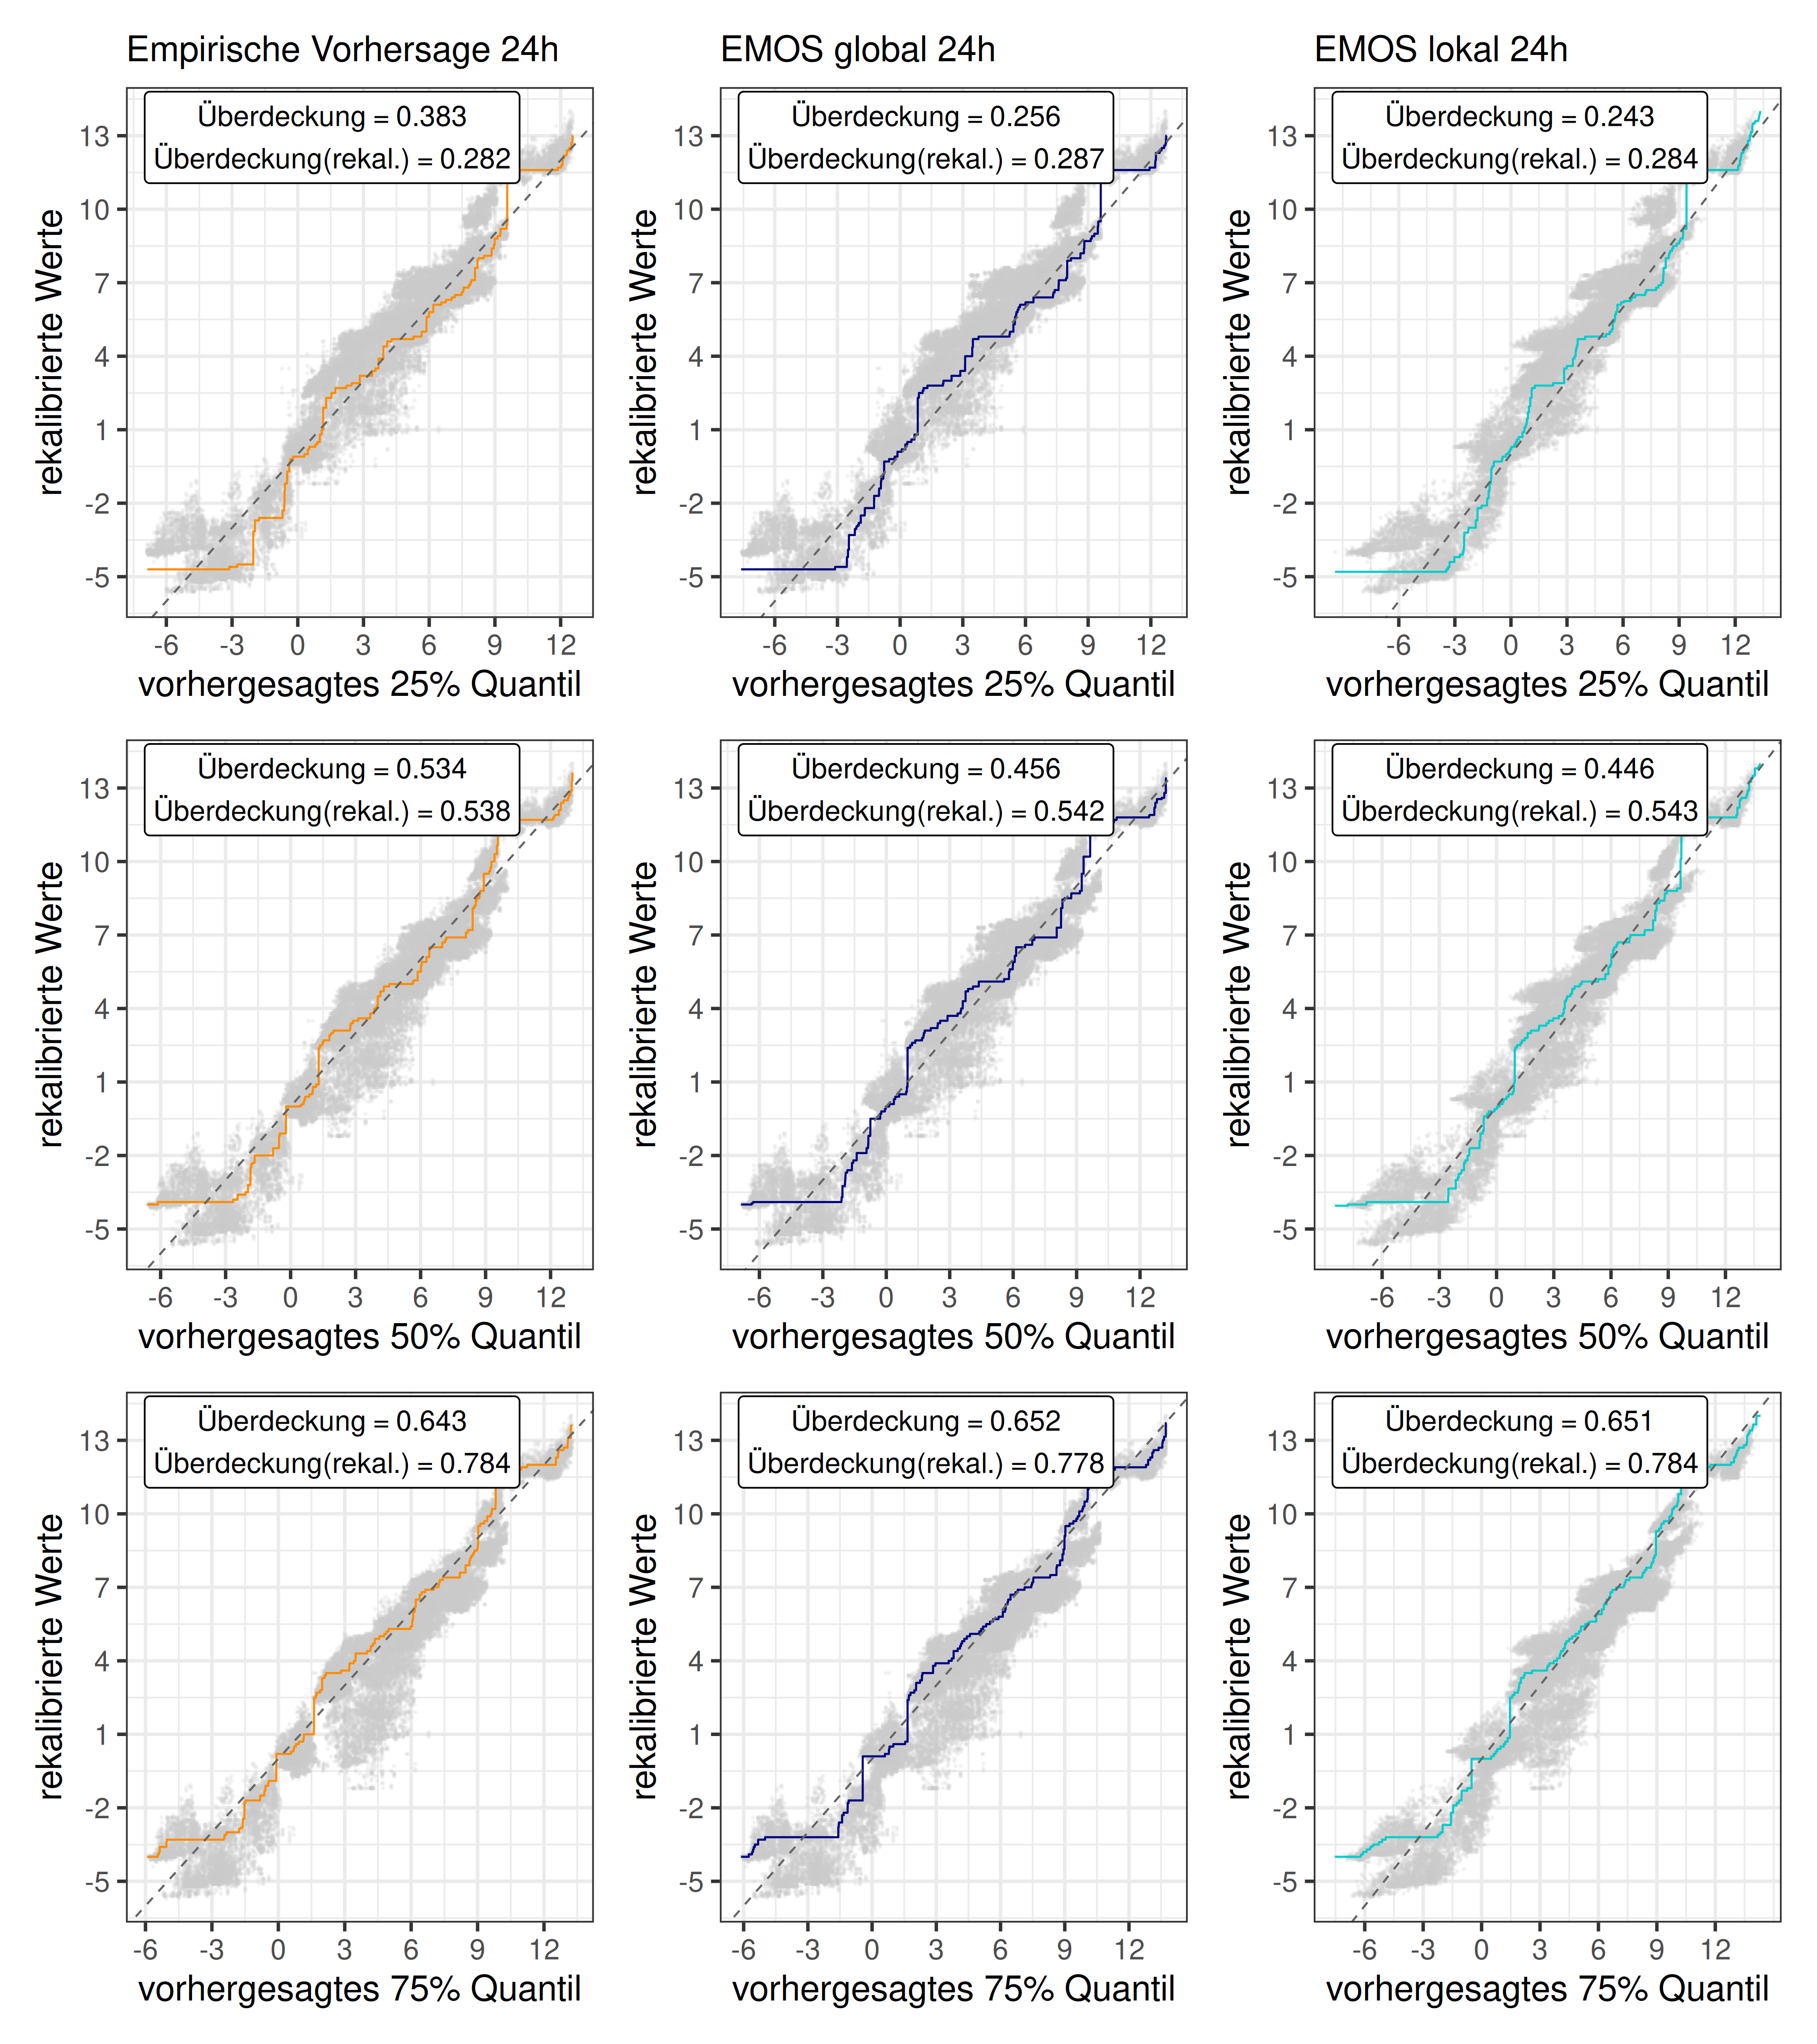
\includegraphics[width=\linewidth]{figs/quant_24_Rplot.png}
    \caption{Reliabilitätsdiagramme der Quantilkalibrierung für den Vorhersagehorizont $24\h$ für die Quantile $25\%$, $50\%$ und $75\%$. Die Plots sind zeilenweise nach Quantilniveau und spaltenweise nach Vorhersageverfahren angeordnet.}
    \label{fig:quant_plot}
\end{figure}

\begin{figure}[!h]
    \centering
    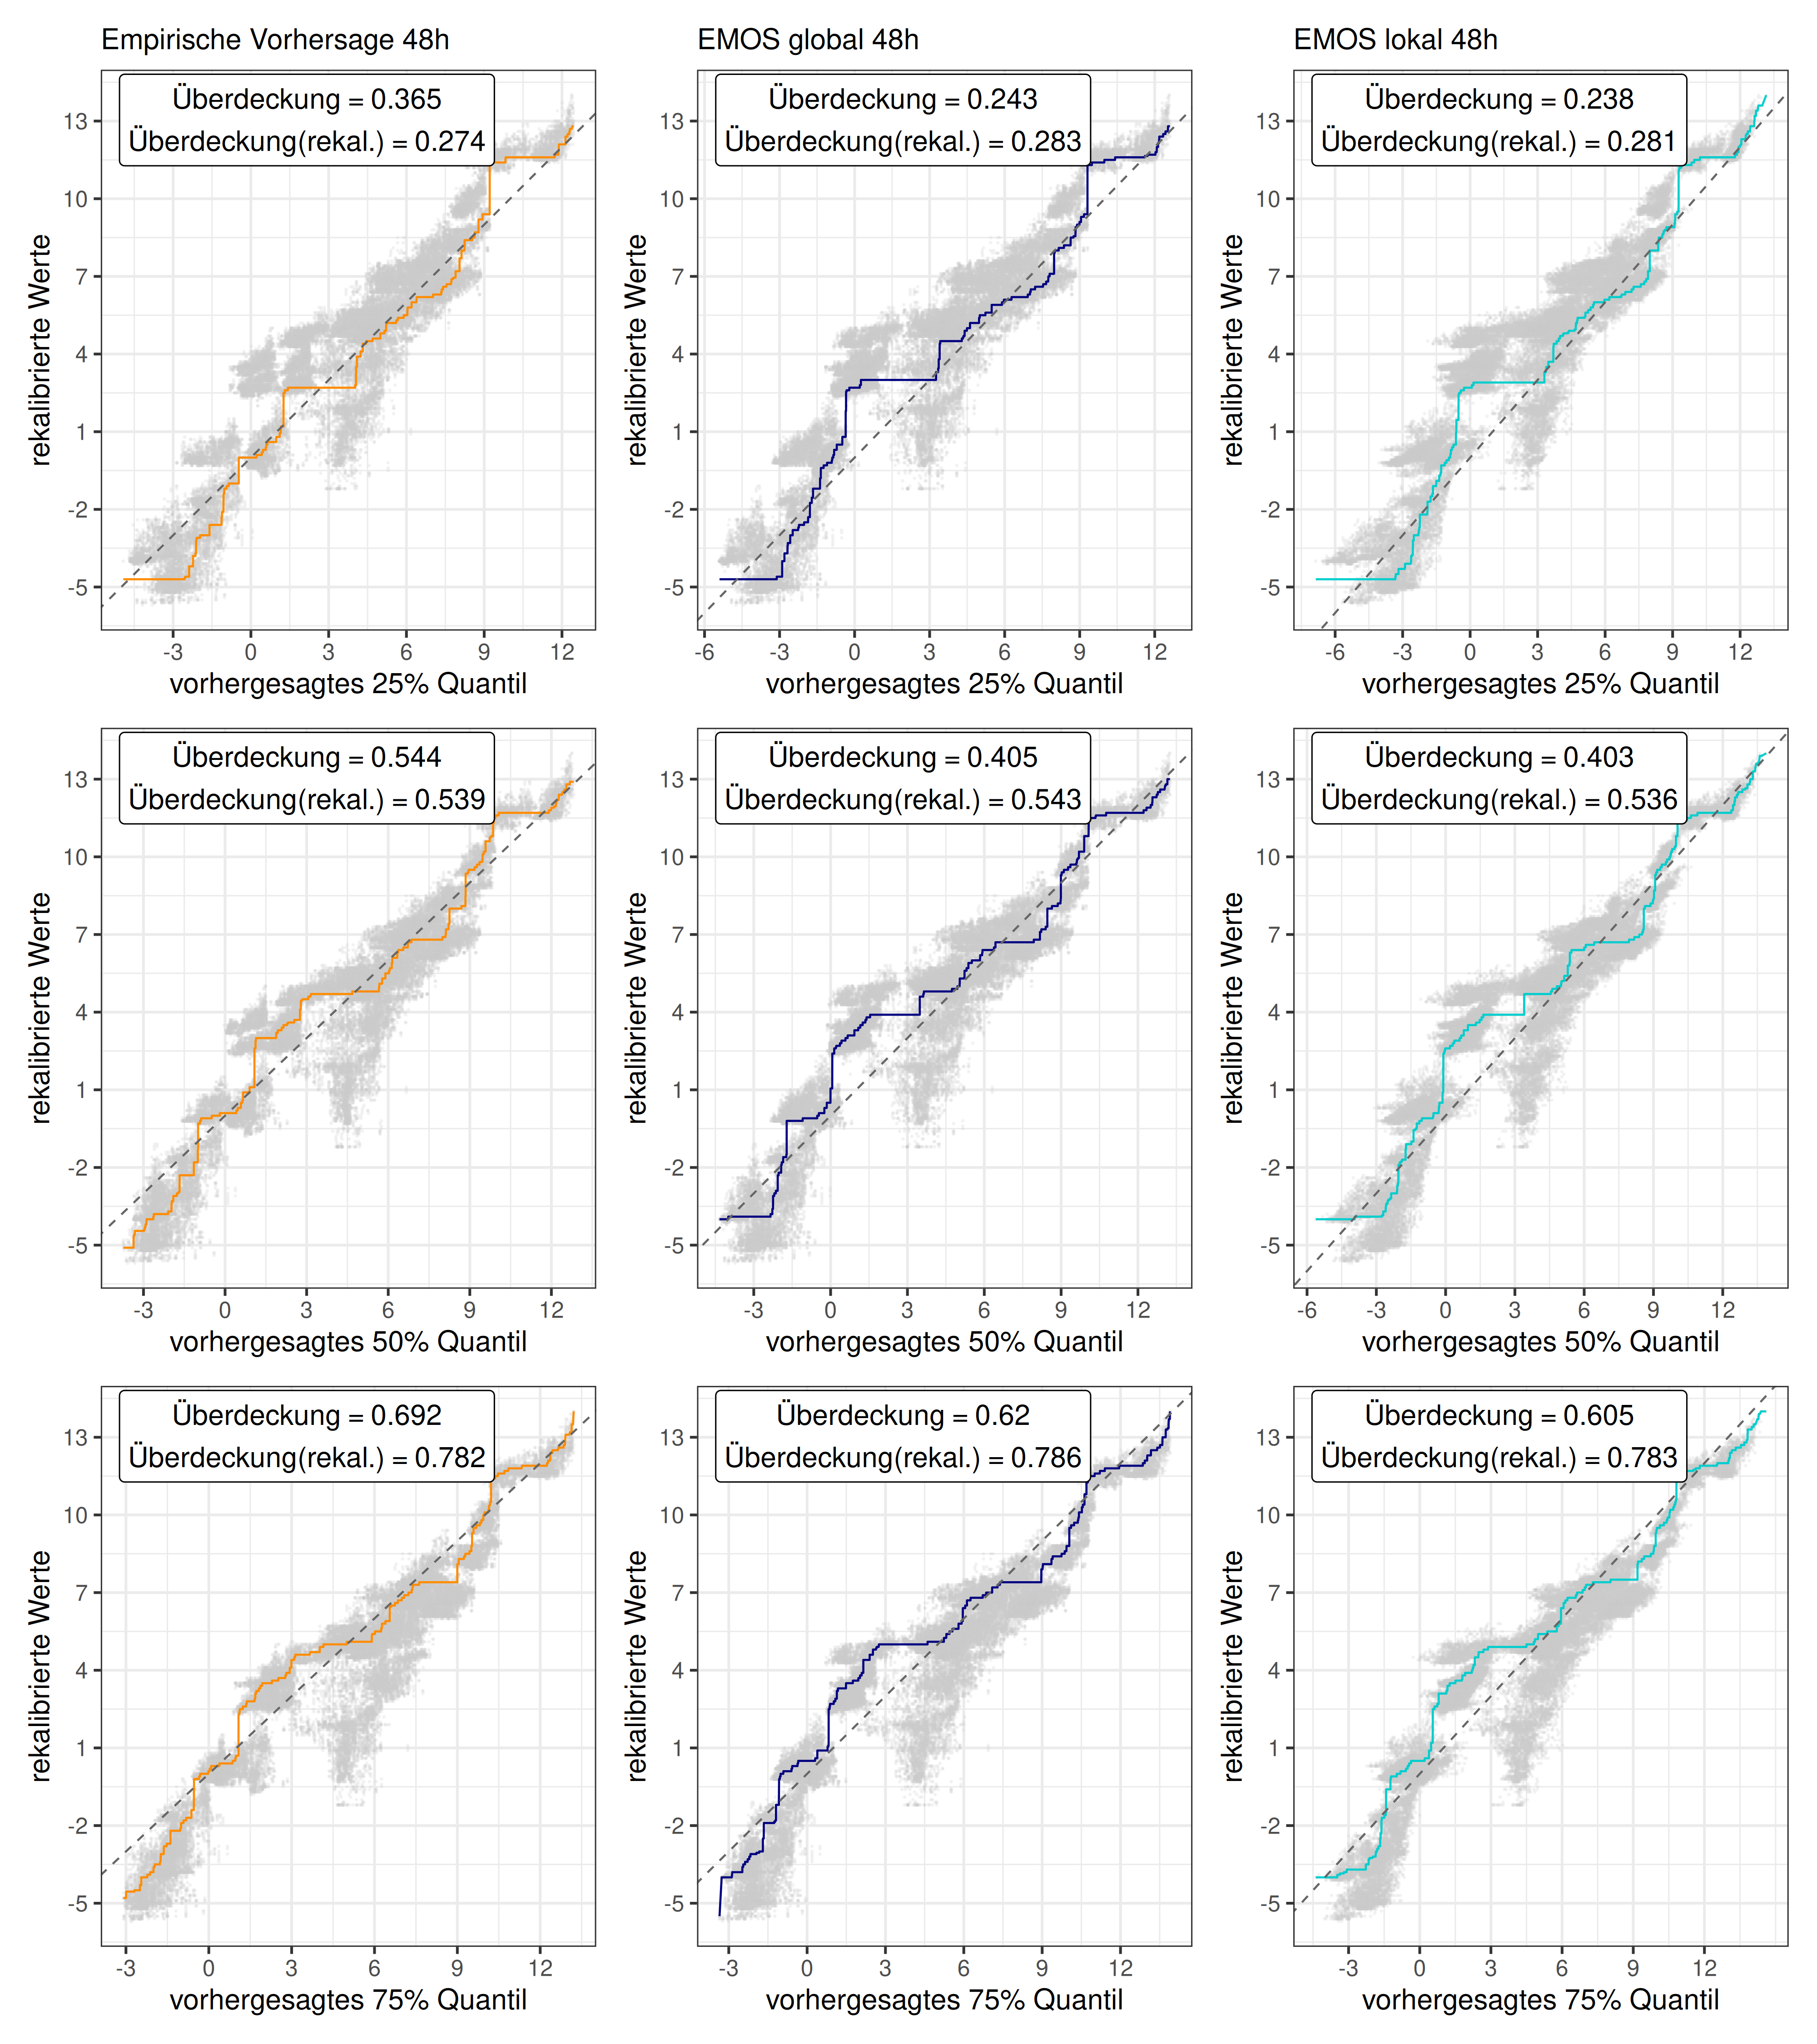
\includegraphics[width=\linewidth]{figs/quant_48_Rplot.png}
    \caption{Reliabilitätsdiagramme der Quantilkalibrierung für den Vorhersagehorizont $48\h$ für die Quantile $25\%$, $50\%$ und $75\%$. Die Plots sind zeilenweise nach Quantilniveau und spaltenweise nach Vorhersageverfahren angeordnet.}
    \label{fig:quant_48_plot}
\end{figure}

Für den Vorhersagehorizont $24\h$ ist über alle drei Vorhersagen hinweg eine ähnliche Fehlerstruktur erkennbar. Insgesamt verlaufen die Kalibrierungsfunktionen im zentralen Wertebereich relativ nahe an der Diagonalen. Abweichungen treten insbesondere in den unteren Randbereichen auf. Im Bereich kleiner vorhergesagter Quantile zeigen sich längere horizontale Segmente der Kalibrierungsfunktion. Dies deutet auf eine erhöhte Anzahl an Monotonieverletzungen hin, wodurch die Quantilkalibrierung im unteren Wertebereich nicht optimal ist. Vorhergesagte Quantile unterhalb von etwa $-5\C$ unterschätzen die beobachteten Quantile, während Quantilvorhersagen zwischen etwa $-4\C$ und $0\C$ sie überschätzen. Darüber hinaus zeigen die EMOS-Vorhersagen im mittleren Temperaturbereich zwischen etwa $1\C$ und $5\C$ eine leichte Unterschätzung der bedingten beobachteten Quantile.

Zum Vorhersagehorizont $48\h$ zeigt sich ebenfalls eine ähnliche Struktur über alle Quantile und Vorhersagen. Im Bereich kleiner vorhergesagter Quantile sind die horizontalen Abschnitte zwar weniger ausgeprägt als beim $24\h$ Horizont, dennoch liegen die rekalibrierten Werte überwiegend unterhalb der Diagonalen. Die vorhergesagten Quantile in diesem Wertebereich überschätzten somit die beobachteten Quantile. Auffällig ist erneut, dass die Kalibrierungskurven der EMOS-Vorhersagen im Temperaturbereich zwischen $0\C$ und $5\C$ oberhalb der Diagonalen liegen. Diese Abweichung ist im Vergleich zum $24\h$ Horizont deutlich stärker ausgeprägt. Das weist auf eine Unterschätzung der beobachteten Quantile in diesem Temperaturbereich hin.


%Marginale Kalibrierung:
%24 h: alle Vorhersagen ähnlich gut, empirische Vorhersage mit geringsten Abweichungen
%48 h: EMOS schlechter als empirische Vorhersage
%Probabilistische Kalibrierung:
%24 h: EMOS insgesamt besser als Rohensemble (weniger Unterdispersion), aber mit negativem Bias
%48 h: EMOS keine Verbesserung 
%Quantilkalibrierung:
%24 h: ähnliche Qualität, empirische Vorhersage eventuell leicht besser (wegen  Abweichungen im Bereich 1{-}5
%48 h: empirische Vorhersage besser aufgrund geringerer systematischer Abweichungen im Bereich 1{-}5


\FloatBarrier
\section{Scores} \label{sec:res_scores}

\subsection{CRPS und Quantilscore}


Tabelle \ref{tab:crps} fasst den mittleren CRPS der Vorhersagen über alle Zeitpunkte und Gitterzellen zusammen. Die Scores reichen von minimal $0.05\C$ bis maximal $5.53\C$. Für den $24\h$ Horizont unterscheiden sich die Vorhersagen mit einem Wert von etwa $0.6\C$ kaum, nur das die lokale Vorhersage einen geringeren maximalen Score aufweist. Für den $48\h$ Horizont liefert die empirische Vorhersage die besten Ergebnisse ($0.81\C$). Die EMOS Vorhersagen sind um etwa $0.1\C$ schlechter.

\begin{table}[!h]
\caption{CRPS der Vorhersagen.}
\centering
\newcolumntype{L}{>{\raggedright\arraybackslash}X}
\newcolumntype{R}{>{\raggedleft\arraybackslash}X}
\begin{tabularx}{0.9\textwidth}{L L R R R R}
\toprule
Horizont & Methode & CRPS & Min & Max & $q_{25}$--$q_{75}$\\
\midrule
\addlinespace[0.3em]
\multicolumn{6}{l}{24 h\,h}\\
& empirisch & 0.64 & 0.05 & 5.53 & 0.23--0.90\\
& global & 0.63 & 0.16 & 5.09 & 0.28--0.83\\
& lokal & 0.62 & 0.09 & 3.80 & 0.26--0.83\\
\addlinespace[0.3em]
\multicolumn{6}{l}{48 h\,h}\\
& empirisch & 0.81 & 0.05 & 5.61 & 0.30--1.13\\
& global & 0.90 & 0.16 & 5.05 & 0.37--1.30\\
& lokal & 0.91 & 0.09 & 4.90 & 0.37--1.32\\
\bottomrule
\end{tabularx}
\label{tab:crps}
\end{table}


Als Nächstes untersuchen wir, wie sich die Güte der Vorhersagen über verschiedene Quantilniveaus hinweg verhält. Dazu zeigt Abbildung \ref{fig:qs_plot} den verdoppelten mittleren Quantilscore in Abhängigkeit vom Quantilniveau der Vorhersagen, sodass die Fläche unter der Kurve dem mittleren CRPS der jeweiligen Vorhersage entspricht (vgl. Abschnitt \ref{seq:crps_qs}). Dadurch lässt sich identifizieren, welche Quantilbereiche Unterschiede im CRPS verursachen. Es zeigt sich ein typischer umgekehrter U-förmige Verlauf des Quantilscores: Die Randquantile weisen geringere Scores auf, während die größten Beiträge zum CRPS aus dem mittleren Quantilbereich stammen.

Für den Vorhersagehorizont $24\h$ unterscheiden sich die Verfahren insgesamt nur geringfügig: Die größten Abweichungen treten im unteren und mittleren Quantilbereich auf. Während die EMOS-Vorhersagen im unteren Bereich geringfügig bessere Quantilscores aufweisen, erzielt die empirische Vorhersage im mittleren Bereich leicht bessere Werte. Für den Vorhersagehorizont von $48\h$ sind die EMOS-Vorhersagen bis etwa zum $25\%$-Quantilniveau zwar ebenfalls geringfügig überlegen, weisen jedoch für alle höheren Quantilniveaus deutlich schlechtere Scores auf. Die Defizite der EMOS-Vorhersagen diesen Horizonts liegen somit insbesondere in den höheren Quantilbereichen.

%Dies erklärt insbesondere die erhöhten Quantilscores im Bereich hoher Quantile, da extreme Beobachtungen durch die Vorhersagen nicht ausreichend abgebildet werden.
 
\begin{figure}[!h]
    \centering
    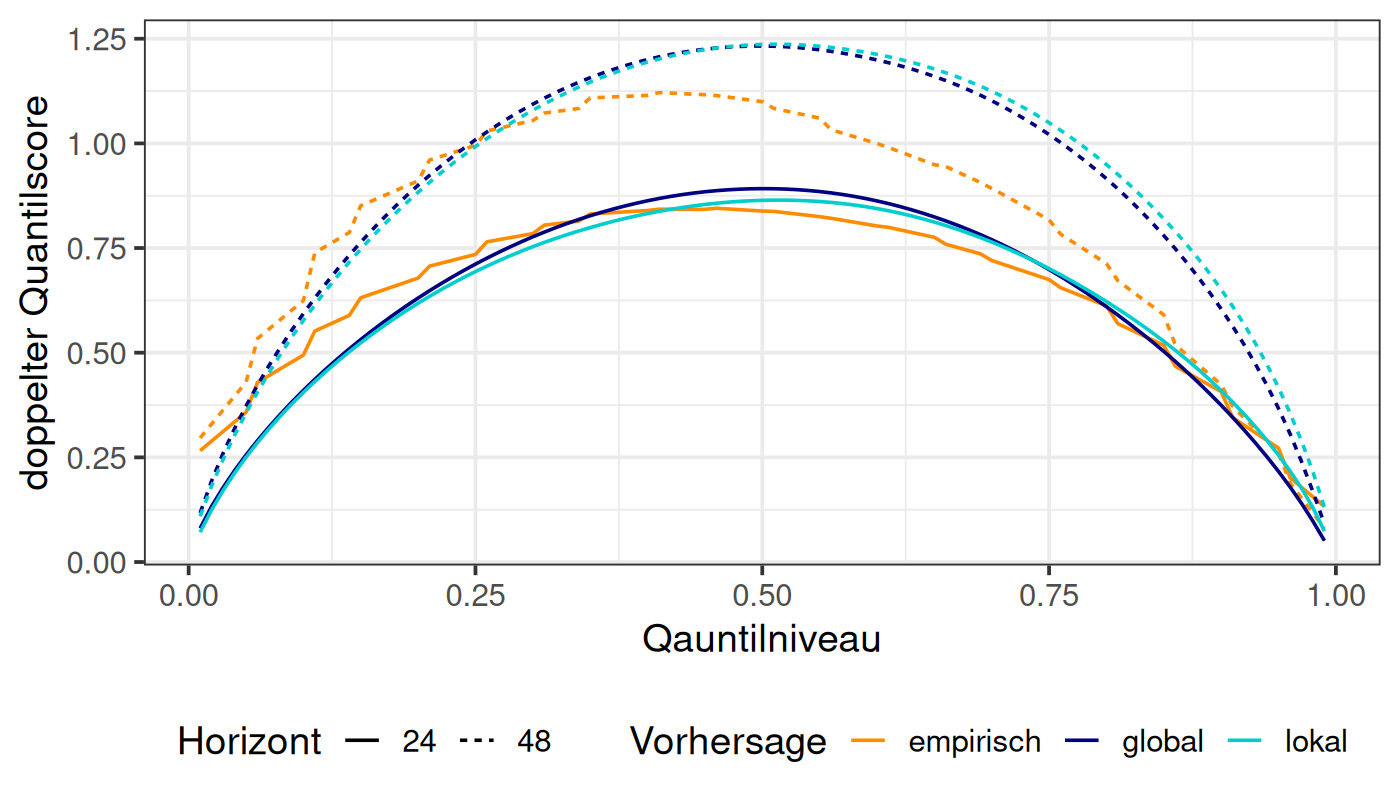
\includegraphics[width=.75\linewidth]{figs/qs_error_curve_Rplot.png}
    \caption{Doppelter Quantilscore für verschiedene Qauntilniveaus der Vorhersagen.}
    \label{fig:qs_plot}
\end{figure}




\subsection{Score Zerlegung}
Zur Analyse von Quellen der Vorhersagequalität wurde der mittlere CRPS, wie in Kapitel \ref{chap:score_decomp} erläutert, in die Komponenten Unsicherheit (UNC), Diskriminationsfähigkeit (DSC) und Misskalibrierung (MCB) zerlegt. Zusätzlich wurde der mittlere Quantilscore für die Niveaus $25\%$, $50\%$ und $75\%$ sowie die extremen Quantile $5\%$ und $95\%$ ebenfalls zerlegt, um die Vorhersagequalität für verschiedene Bereiche der Vorhersageverteilung zu analysieren. Der Quantilscore ist wieder verdoppelt, um ihn besser mit dem CRPS vergleichen zu können (vgl. \eqref{eq:crps_qs}).

%\todo{hier vielleicht mit shape und color statt textstring arbeiten}
\begin{figure}[!htbp]
    \centering
    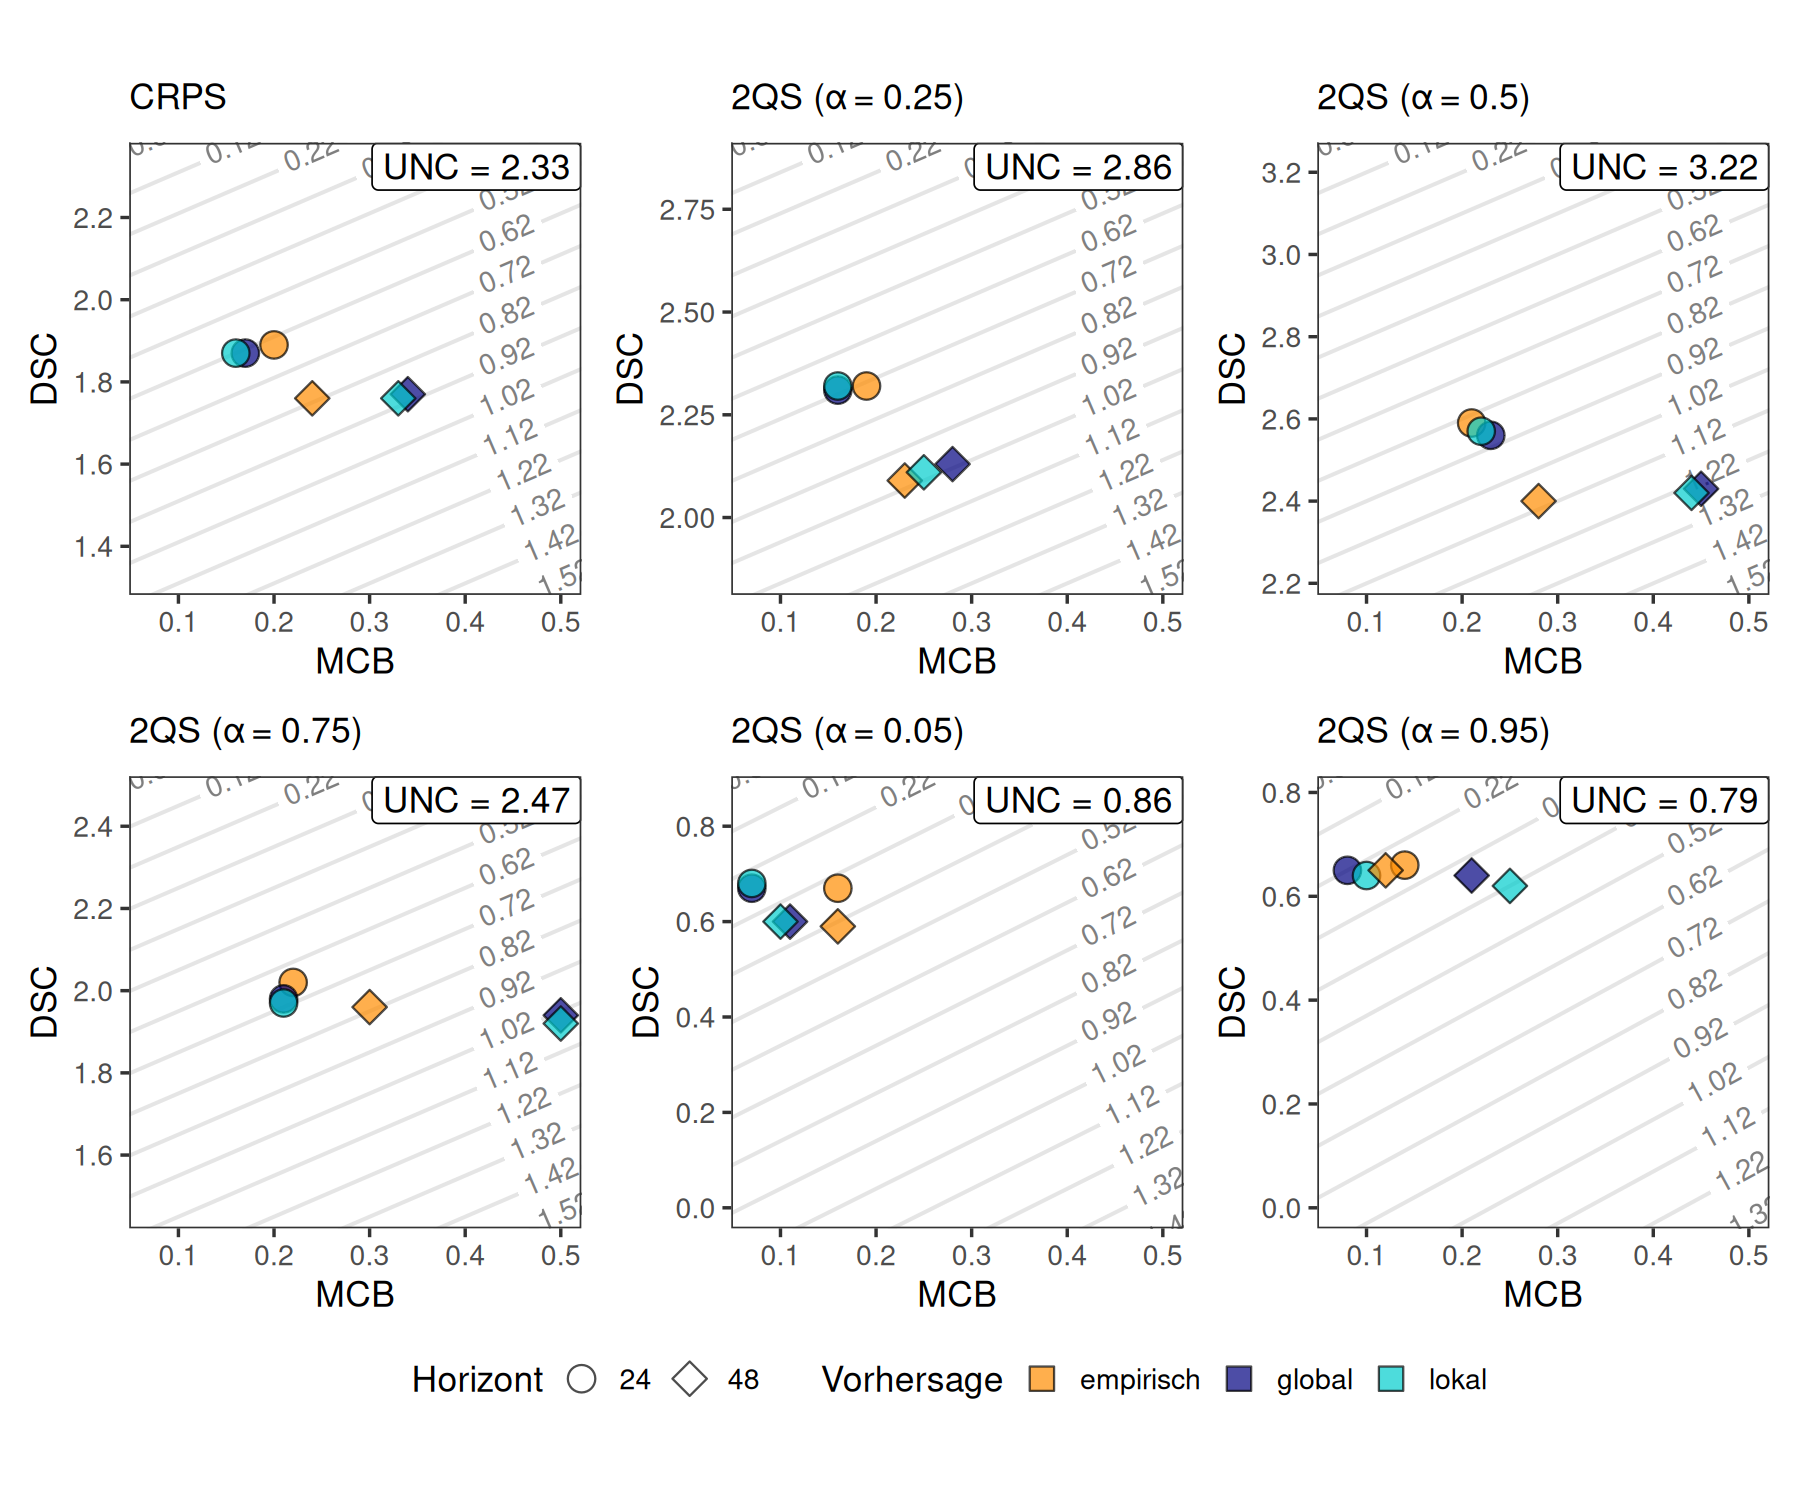
\includegraphics[width=1\linewidth]{figs/decomp_Rplot.png}
    \caption{Zerlegungsdiagramme der Scores.}
    \label{fig:decomp_plot}
\end{figure}

%Für $48\h$ verschlechtern sich sowohl Kalibrierung als auch Diskriminierung.
Abbildung \ref{fig:decomp_plot} zeigt die Zerlegungsdiagramme für die verschiedenen Scores. Die $24\h$ Vorhersagen zeigen für fast alle Scores eine bessere Kalibrierung und Diskriminierung als die $48\h$ Vorhersagen vor allem hinsichtlich Kalibrierung. Zudem bestehen zwischen der globalen und der lokalen Vorhersage wieder geringe Unterschiede.

Der CRPS zeigt für $24\h$ nur geringe Unterschiede zwischen den Vorhersagen, wobei die EMOS-Vorhersagen minimal besser kalibriert, jedoch leicht schlechter diskriminierend sind. Für $48\h$ weisen die EMOS-Vorhersagen eine ähnliche Diskriminations\-fähigkeit wie die empirischen Vorhersage auf, jedoch sind sie schlechter kalibriert, wodurch der Gesamtscore schlechter wird. Die Quantilscores zeigen ein ähnliches Muster wie der CRPS, jedoch mit etwas größeren Scoreunterschieden. Beim $25\%$-Quantil sind die EMOS-Vorhersagen für den $48\h$ Horizont ähnlich der empirischen Vorhersage kalibriert, während sie beim $50\%$- und $75\%$-Quantil eine auffallend schlechtere Kalibrierung aufweisen. Die extremen Quantile ($5\%$ und $95\%$) zeigen die niedrigsten Scores, weisen jedoch auch die geringste Unsicherheitskomponente auf. Beim $5\%$-Quantil sind alle EMOS-Vorhersagen leicht besser kalibriert als die empirischen Vorhersagen. Beim $95\%$-Quantil entspricht das Verhalten weitgehend dem des $75\%$-Quantils, jedoch sind die Unterschiede in der Kalibrierung nicht so stark ausgeprägt. Die genauen Zahlen der Zerlegung mit dem Skill Score sind in Appendix \ref{seq:decomp-table} dargestellt.


\subsection{Räumliche und zeitliche Dynamiken im CRPS} \label{sec:res_spat_time}
Die Analyse der räumlichen und zeitlichen Dynamiken der Vorhersagen im CRPS ermöglicht eine Bewertung, wie sich die Qualität der Temperaturvorhersagen über verschiedene Regionen und Vorhersagezeiträume hinweg verändert.

Abbildung \ref{fig:crps_day_plot} zeigt den mittleren CRPS über die Tage des Evaluationszeitraums getrennt nach Vorhersage. Über die verschiedenen Tage sind die Fehlerwerte ungleichmäßig verteilt, wobei sowohl Phasen mit vergleichsweise niedrigen als auch mit erhöhten CRPS-Werten auftreten. Die Scores reichen von $0.2\C$ bis über $2.5\C$. Wieder sind für den $48\h$ Horizont die Fehler deutlich größer. Auch zeigen die EMOS-Vorhersagen jeweils ein nahezu identisches Profil.

\begin{figure}[h]
    \centering
    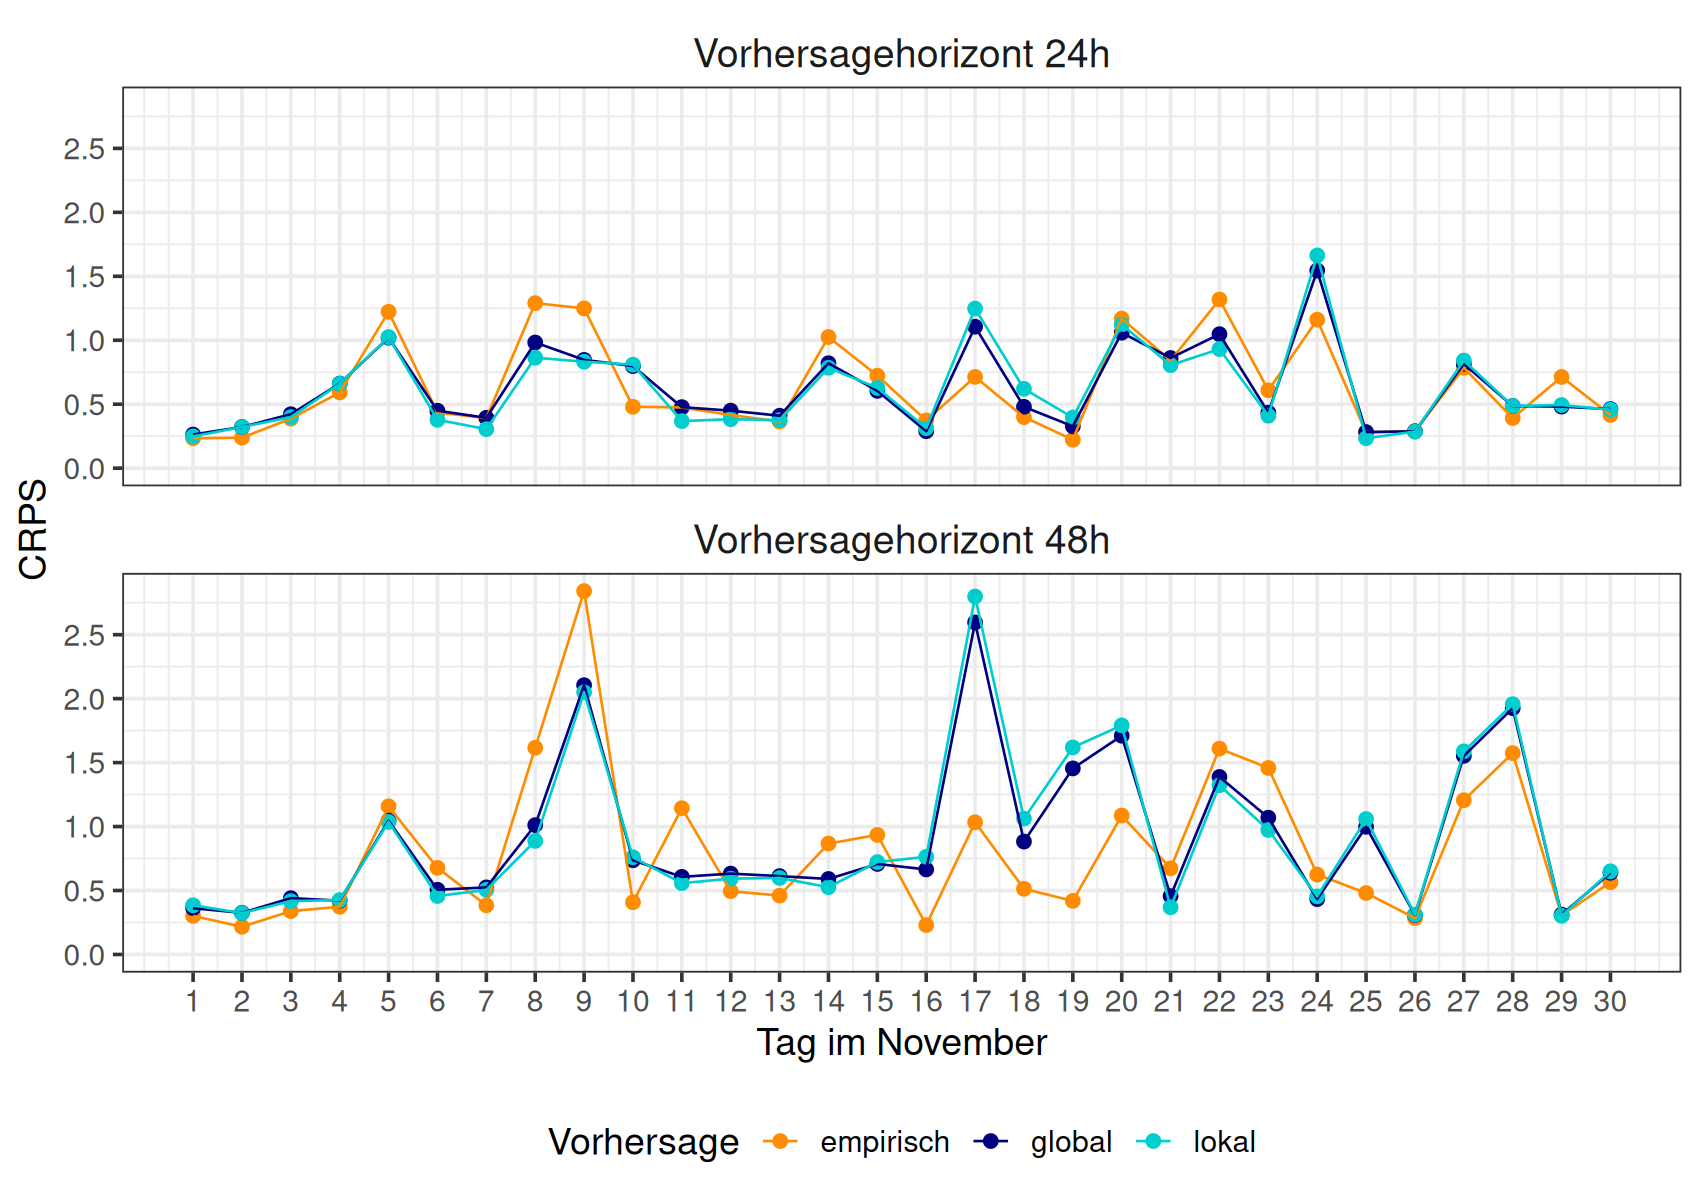
\includegraphics[width=0.9\linewidth]{figs/crps_time.png}
    \caption{Zeitlicher Verlauf des mittleren CRPS über den Evaluationszeitraum.}
    \label{fig:crps_day_plot}
\end{figure}

Für den $24\h$ Horizont liegen alle Vorhersagen recht nah beieinander, wohingegen sich beim $48\h$ die empirische und die EMOS-Vorhersagen stärker voneinander unterscheiden. Besonders fällt auf, dass über beide Vorhersagehorizonte die EMOS-Vorhersagen am 17.11. Scores besitzen, die schlechter sind als die der korrespondierenden empirischen Vorhersagen. Dieses Muster lässt sich durch den negativen Bias der EMOS-Vorhersagen erklären (vgl. Abschnitt \ref{sec:res_pit_cal}). So fällt im Vergleich mit Abbildung \ref{fig:icon_time} auf, dass die EMOS-Vorhersagen tendenziell einen höheren CRPS aufweisen, wenn viele Ensemblemitglieder unter der HOSTRADA-Temperatur liegen, also zu niedrig sind. Liegen viele Ensemblemitglieder unter der HOSTRADA-Temperatur, führt der negative Bias der EMOS-Vorhersage zu einer stärkeren Unterschätzung der Temperatur und somit zu einer größeren Abweichung von der beobachteten Temperatur, was sich in einem höheren CRPS widerspiegelt. Die empirische Vorhersage weist dagegen bei beiden Vorhersagehorizonten am 9.11. und 22.11. die höchsten Scores auf. Der Vergleich mit Abbildung \ref{fig:icon_time} zeigt, dass die Ensemblemitglieder an diesen Tagen die HOSTRADA-Temperatur tendenziell überschätzen.

Um räumliche Variationen in der Vorhersagegüte zu erfassen, ist in Abbildung \ref{fig:crps_cells} der mittlere CRPS pro Gitterzelle dargestellt. Für den Horizont $24\h$ weisen alle Vorhersagen überwiegend niedrige CRPS-Werte zwischen etwa $0.4\C$ und $0.8\C$ auf, was auf eine gute Übereinstimmung zwischen Vorhersage und Beobachtung hindeutet. Bei $48\h$ steigen die CRPS-Werte in allen Vorhersagen deutlich an.

Über alle Vorhersagen hinweg lassen sich folgende räumliche Muster erkennen. Im östlichen bzw. südöstlichen Berliner Randgebiet treten erhöhte CRPS-Werte auf, während im westlichen und zentralen Bereich geringere Fehler beobachtet werden. Insbesondere fallen bei den empirischen Vorhersagen Fehlerhotspots auf. Diese korrespondieren mit Gewässern in Berlin, dem Teglersee (links oben), der Havel (links unten) und dem Großen Müggelsee (rechts unten) (siehe Abbildung \ref{fig:berlin_spat}). Hier unterscheidet sich die lokale Vorhersage von den anderen Verfahren. Sie glättet die zuvor beobachteten Hotspots räumlich.

Diese räumliche Systematik deutet nicht notwendig auf Defizite in der Vorhersagequalität hin, sondern könnte auf Unterschiede in der Modellierung der zugrunde liegenden Datensätze zurückzuführen sein. HOSTRADA stellt einen rasterbasierten Beobachtungsdatensatz dar, dessen Temperaturfelder überwiegend durch statistische Interpolation von Stationsmessungen erzeugt werden \parencite{krahenmann_high-resolution_2018}. Die Unterscheidung zwischen Wasser und Land erfolgt dabei über die Rauhigkeit der Fläche, wobei Wasserflächen eine sehr geringe Rauhigkeit zugewiesen bekommen. Dies beeinflusst die Windgeschwindigkeit und dadurch auch die Temperatur. Demgegenüber basiert ICON-D2-ESP auf einem numerischen Wettermodell, in dem die Eigenschaften der Oberflächen explizit berücksichtigt werden \parencite{reinert2025icon_dwd}. Aufgrund der nativen räumlichen Auflösung von 2 km können Gewässerränder jedoch nur grob abgebildet werden, sodass einzelne Gitterzellen sowohl Land- als auch Wassereigenschaften enthalten können. Unterschiede oder Unsicherheiten bei der Darstellung dieser Oberflächeneigenschaften können sich ebenfalls auf die simulierten Temperaturen auswirken. Diese Aspekte wurden mir auf Anfrage von Arne Spitzer vom Deutscher Wetterdienst (DWD), per E-Mail erläutert (persönliche Kommunikation, 2026).

Vor diesem Hintergrund ist es plausibel, dass Gewässer wie der Große Müggelsee im ICON-D2-ESP einen stärkeren Einfluss auf das Temperaturfeld ausüben als im HOSTRADA, der diese möglicherweise nur eingeschränkt abbildet. Ein Indiz hierfür ist, dass in Abbildung \ref{fig:nov_temp_spat} die Gewässer in den Temperaturbeobachtungen nicht sichtbar werden. Die an den Gewässern auftretenden erhöhten CRPS-Werte der Vorhersagen könnten somit zumindest teilweise auf Unterschiede in der Darstellung der Gewässer zwischen den beiden Datensätzen zurückzuführen sein.

\begin{figure}[h]
    \centering
    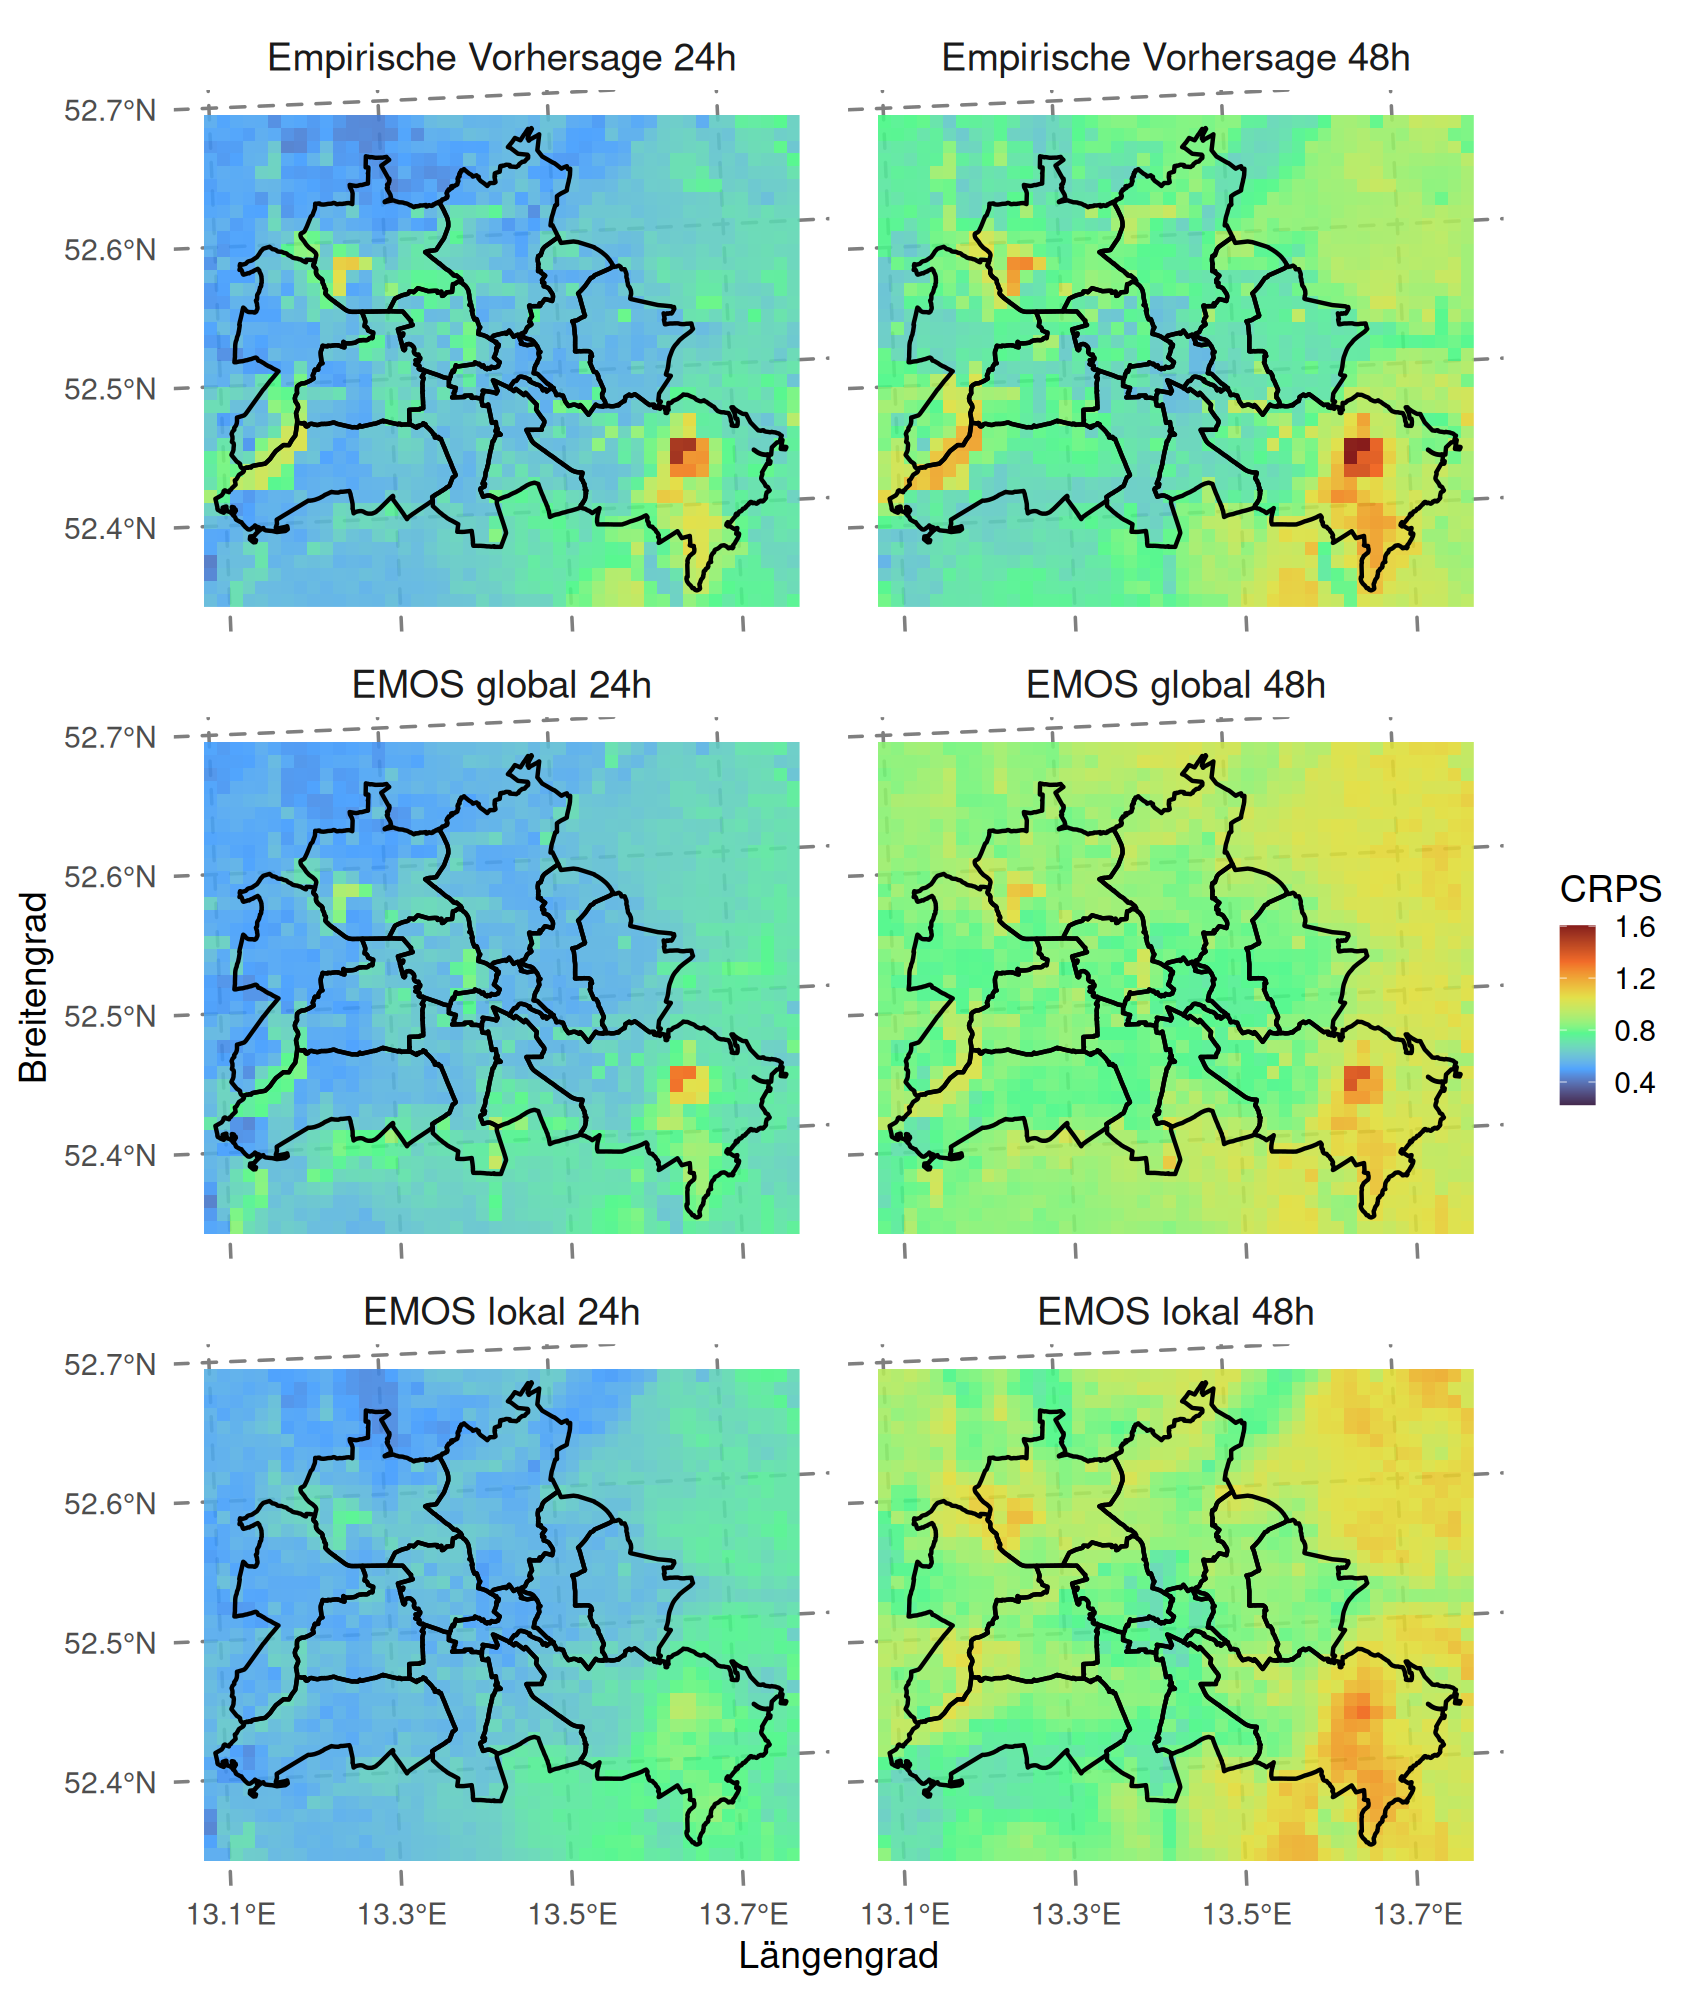
\includegraphics[width=0.89\linewidth]{figs/crps_spat.png}
    \caption{Mittlerer CRPS der Gitterzellen über den Evaluationszeitraum.}
    \label{fig:crps_cells}
\end{figure}


\FloatBarrier
\section{Zusammenfassung} \label{sec:res_sum}
Zusammenfassend zeigen die verschiedenen Kalibrierungsbegriffe ein differenziertes Bild. Die beiden EMOS-Vorhersagen unterscheiden sich dabei nur geringfügig und können daher weitgehend gemeinsam betrachtet werden. Hinsichtlich der marginalen Kalibrierung weisen für den $24\h$ Horizont alle betrachteten Vorhersagen eine vergleichbare Qualität auf, wobei die empirische Vorhersage die geringsten Abweichungen von der Idealgeraden in Abbildung \ref{fig:marg_plot} zeigt. Für den $48\h$ Horizont weisen die EMOS-Vorhersagen hingegen größere Abweichungen auf als die empirische Vorhersage.

Bei der probabilistischen Kalibrierung zeigt sich für den $24\h$ Horizont ein Vorteil der EMOS-Vorhersagen gegenüber der empirischen Vorhersage, weil die Unterdispersion der empirischen Vorhersage reduziert wird. Gleichzeitig tritt jedoch ein negativer Bias auf. Für den $48\h$ Horizont führt die EMOS-Vorhersage hingegen zu keiner Verbesserung der probabilistischen Kalibrierung, weil die Reduktion der Unterdispersion durch den stärkeren negativen Bias ausgeglichen wird.

Auch hinsichtlich der Quantilkalibrierung zeigt sich kein einheitlicher Vorteil der EMOS-Vorhersagen. Für den $24\h$ Horizont ist die Kalibrierung der betrachteten Vorhersagen insgesamt ähnlich. Für den $48\h$ Horizont weist die empirische Vorhersage hingegen eine bessere Quantilkalibrierung auf, weil bei den EMOS-Vorhersagen im Wertebereich von etwa $1\C$ bis $5\C$ Abweichungen von der Idealgraden auftreten. Insgesamt sind die betrachteten Vorhersagen als ausreichend kalibriert einzustufen, weisen jedoch weiterhin Abweichungen auf, insbesondere für den längeren Vorhersagehorizont von $48\h$.

Die Scoreanalysen bestätigen die bessere Vorhersagegüte des $24\h$ Horizonts gegenüber dem $48\h$ Horizont. Für den $24\h$ Horizont unterscheiden sich die Vorhersagen hinsichtlich ihrer Gesamtgüte nicht bedeutsam. Für den $48\h$ Horizont liefert hingegen die empirische Vorhersage die besten Ergebnisse. Insbesondere für Quantile oberhalb von etwa $25\%$ weist sie bessere Quantilscores auf. 

Die Zerlegung des CRPS zeigt, dass die schlechteren CRPS-Werte der EMOS-Vor\-hersagen hauptsächlich auf Kalibrierungs\-fehler zurückzuführen sind, insbesondere in den zentralen Quantilbereichen von $50\%$ und $75\%$. Die Diskriminationsfähigkeit unterscheidet sich hingegen kaum von der empirischen Vorhersage. Genauso wie bei der Kalibrierungsanalyse, ergeben sich für die globalen und die lokalen EMOS-Variante über die verschiedenen Analysen hinweg nur geringe Unterschiede.

Die zeitliche Analyse des CRPS zeigt, dass die Vorhersagequalität stark zwischen den Tagen variiert. Dabei treten einzelne Tage mit besonders hohen Fehlern hervor Beispielsweise der 17.11 oder der 9.11 .

Räumlich fallen insbesondere an den Gewässern Berlins erhöhte Fehlerwerte auf. Diese räumlichen Unterschiede könnten auf die unterschiedliche Modellierung und Repräsentation von Land- und Wasserflächen in den zugrunde liegenden Modellansätzen der Daten zurückzuführen sein. Die lokale EMOS-Vorhersage unterscheidet sich hier von den übrigen Vorhersagen, weil sie die auftretenden Fehlerhotspots räumlich glättet. Dieser Vorteil spiegelt sich jedoch nicht in einer insgesamt besseren Vorhersagegüte im Sinne eines bedeutsamen Unterschieds im CRPS wider. 

Bezogen auf die aufgestellten Vermutungen in Abschnitt \ref{sec:meth_hp} können wir festhalten, dass die Vermutung einer abnehmenden Vorhersagegüte mit zunehmendem Vorhersagehorizont bestätigt wird. Ebenso bestätigt sich die Vermutung, dass die empirischen Vorhersagen typische Eigenschaften von Rohensembles, insbesondere Unterdispersion, jedoch kaum Bias aufweisen. Die Vermutung, dass das EMOS-Postprocessing grundsätzlich zu einer verbesserten Kalibrierung führt, bestätigt sich jedoch nicht. Vorteile dieses Vorgehens beschränken sich auf den $24\h$ Horizont und die probabilistische Kalibrierung. Die Nachteile zeigen sich beim $48\h$ Horizont, vor allem in Form eines negativen Bias. Des Weiteren lässt sich ein Vorteil der lokalen gegenüber der globalen EMOS-Variante nicht feststellen. Die letzte Vermutung, dass sich die Diskriminationsfähigkeit aufgrund der gemeinsamen Informationsgrundlage der Vorhersagen nur geringfügig unterscheidet, wird hingegen durch die Ergebnisse der Score Zerlegung weitestgehend gestützt. Insgesamt zeigen die somit Ergebnisse entgegen der ursprünglichen Vermutung keinen generellen Vorteil des statistischen Postprocessings.


\chapter{Diskussion} \label{chap:discuss}
In diesem Kapitel werden die Ergebnisse der Arbeit eingeordnet und die verwendeten Evaluationsmethoden reflektiert. Zunächst werden auffällige Ergebnisse des praktischen Teils im Hinblick auf das eingesetzte Postprocessing sowie die Datengrundlagen diskutiert. Anschließend liegt der Schwerpunkt auf der praktischen Anwendbarkeit und Aussagekraft der verwendeten Evaluationsmethoden. Abschließend werden die Limitationen der Arbeit thematisiert und mögliche Ansatzpunkte für weiterführende Untersuchungen aufgezeigt.

\section{Ergebnisdiskussion} \label{sec:disc_res}

\subsection{Einordnung des Postprocessings}

Das auffälligste Ergebnis der praktischen Untersuchung der Berliner Temperaturvorhersagen war, dass das EMOS-Postprocessing nicht zu der erwarteten generellen Verbesserung der Vorhersagequalität geführt hat (vgl. Abschnitt \ref{sec:postproc}). Für den $24\h$ Horizont zeigt sich zwar eine Verbesserung der probabilistischen Kalibrierung durch eine Reduzierung der Unterdispersion der empirischen Vorhersage. Gleichzeitig tritt jedoch ein negativer Bias auf, der in der empirischen Vorhersage nicht zu beobachten war. Für den $48\h$ Horizont überwiegen sogar die Nachteile des Postprocessings, sodass die empirische Vorhersage vor allem auch hinsichtlich des CRPS besser abschneidet.
Insgesamt entsteht dadurch der Eindruck, dass das verwendete EMOS-Verfahren im vorliegenden Datensatz nur begrenzt robust ist. Damit stellt sich die Frage, warum das Postprocessing die erwartete Verbesserung nicht erzielt.

Für diese Ergebnisse kommen mehrere Erklärungen in Betracht. Zum einen könnte das verwendete Trainingsfenster von 30 Tagen ungünstig gewählt sein, weil es entweder zu kurz ist, um stabile Schätzungen zu ermöglichen, oder zu lang, um aktuelle saisonale Veränderungen ausreichend zu erfassen. Im November können aufgrund möglicher meteorologischer Übergänge zwischen Herbst und Winter Veränderungen in den Temperaturverteilungen auftreten, die durch ein 30-tägiges gleitendes Trainingsfenster eventuell nicht adäquat abgebildet werden konnten. Unter diesen Bedingungen könnte ein einfacheres Postprocessing, das sich auf die Korrektur der Ensemble-Dispersion beschränkt und den Mittelwert unverändert lässt, robuster sein. Die Ergebnisse verdeutlichen damit grundsätzlich, dass Postprocessing der Ensemblevorhersagen nicht automatisch zu einer besseren Vorhersage führt, sondern Methode und Wahl der Trainingsdaten für den jeweiligen Anwendungsfall angepasst und überprüft werden sollten.

\subsection{ICON-D2-EPS vs. HOSTRADA}
Nach aktuellem Stand konnten keine Veröffentlichungen gefunden werden, die ICON-D2-EPS und HOSTRADA direkt miteinander vergleichen. Die vorliegende Arbeit stellt damit einen ersten Versuch dar, HOSTRADA zur Verifikation probabilitischer Vorhersagen auf Basis des ICON-D2-EPS zu nutzen, und zeigt, dass ein solcher Vergleich grundsätzlich möglich ist. Bei der Interpretation der Ergebnisse müssen jedoch verschiedene methodische Aspekte berücksichtigt werden. So können die Projektion der Datensätze auf ein gemeinsames Gitter sowie die unterschiedlichen räumlichen Auflösungen die Vergleichbarkeit beeinflussen.

Bei der Evaluation der räumlichen Güte der Vorhersagen waren vor allem Fehlerhotspots der Temperatur im Bereich von Gewässern auffällig. Diese weisen auf mögliche Unterschiede in der Modellierung hin (siehe Abschnitt \ref{sec:res_spat_time}). Die Ergebnisse können daher auch für den DWD von Interesse sein. Ein weiterführender direkter Vergleich von ICON-D2-EPS und HOSTRADA könnte dazu beitragen, die beobachteten Unterschiede genauer einzuordnen. Insbesondere ein Vergleich der ICON-D2-EPS-Instantanvorhersage mit HOSTRADA sowie Untersuchungen in weiteren Regionen und zu anderen Zeitpunkten, könnten zusätzliche Erkenntnisse liefern, inwieweit diese Unterschiede systematisch sind.


\subsection{Bewertung der angewandten Evaluationsmethoden}

Schließlich ordnen wir ein, wie sich die im theoretischen Teil eingeführten Evaluationsmethoden in der praktischen Anwendung bewährt haben. Die Ergebnisse zeigen, dass sich die verschiedenen Evaluationsmethoden sinnvoll ergänzen. Die graphische Darstellung der marginalen Kalibrierung anhand der Reliabilitätsdiagramme eignet sich als ersten groben Qualitätscheck, während die graphische Darstellung der probabilistischen Kalibrierung besonders hilfreich war, um Unterdispersion und Bias sichtbar zu machen. Das Reliabilitätsdiagramm der Quantilkalibrierung bietet demgegenüber eine detailliertere Betrachtung einzelner Bereiche der vorhergesagten Verteilung und ermöglicht einen direkten Vergleich zwischen vorhergesagten und beobachteten Quantilen. Jedoch erschwert die große Anzahl an Plots eine übersichtliche Bewertung der Ergebnisse.

Während der CRPS eine aggregierte, quantitative Bewertung der Gesamtgüte der vorhergesagten Verteilung liefert, ermöglicht der Quantilscore eine differenziertere Betrachtung einzelner Bereiche dieser Verteilung. Damit ergänzen sich beide Maße. Zusätzlich war die Zerlegung von CRPS und Quantilscore besonders hilfreich, um zu bestätigen, dass die schlechtere Scores der EMOS-Vorhersagen auf Kalibrierungsprobleme zurückzuführen waren. Jedoch ist insbesondere die CRPS-Zerlegung durch die wiederholte Anwendung des PAVA-Verfahrens vergleichsweise rechenintensiv. 

Zusätzlich lieferten die räumlichen und zeitlichen Analysen des CRPS einen zusätzlichen Erkenntnisgewinn, weil dadurch lokale Fehlerhotspots und einzelne Tage mit besonders hohen Fehlern sichtbar wurden. Vor allem erweist sich somit die Kombination verschiedener Methoden als zielführend. Während einzelne Verfahren zunächst einen grundlegenden Überblick oder eine ganzheitliche Bewertung ermöglichen, liefern detailliertere Kalibrierungs- und Zerlegungsmethoden zusätzliche Erkenntnisse über die Ursachen der beobachteten Unterschiede. Für eine praktische Evaluation bietet sich daher ein abgestuftes Vorgehen an, bei dem zunächst einfachere Verfahren eingesetzt und anschließend diese nach Bedarf und Fragestellung durch detailliertere Analysen ergänzt werden. Eine sorgfältige deskriptive Analyse bildet dabei eine wichtige Grundlage, weil sie erste Auffälligkeiten sichtbar macht und somit gezielt das weiterführende Vorgehen informieren kann.

\section{Limitationen und Ausblick}
Im Rahmen dieser Arbeit konnte nur ein begrenzter Ausschnitt der verfügbaren Methoden zur Evaluation probabilistischer Vorhersagen betrachtet werden. Hinsichtlich der Scores konzentrierte sich die Analyse auf den CRPS und den Quantilscore, während im Bereich der Kalibrierung die verschiedenen im theoretischen Teil vorgestellten Ansätze betrachtet wurden. Weitere Scoring-Rules, wie beispielsweise der Log-Score \parencite{gneiting2014probabilistic}, wurden nicht berücksichtigt. Deren Untersuchung wäre jedoch interessant, weil sie Abweichungen unterschiedlich stark gewichten und dadurch zu einer anderen Beurteilung probabilistischer Vorhersagen führen können. Auch Kalibrierungsansätze, die eine stärkere Annäherung an das Konzept der Auto-Kalibrierung ermöglichen, wie z.B. die isotone Kalibrierung \parencite{arnold2025isotonic}, wurden im Rahmen dieser Arbeit nicht besprochen. Eine nähere Verwendung solcher Verfahren bietet somit einen interessanten Ansatzpunkt für weitere Analysen. Darüber hinaus wurde die räumliche und zeitliche Analyse nur ergänzend betrachtet und im theoretischen Teil nicht behandelt. Eine vertiefte Betrachtung könnte hier weitere Zusammenhänge und Muster aufzeigen. Trotz dieser Einschränkungen bilden die vorgestellten Methoden eine breite Grundlage für die Evaluation probabilistischer Vorhersagen, die wesentliche Aspekte abgedeckt.

Weitere Einschränkungen betreffen die im theoretischen Teil beschriebenen Konsistenzbänder für Reliabilitätsdiagramme. Aufgrund der großen Anzahl betrachteter Vorhersagen und Beobachtungen fielen diese im praktischen Teil sehr schmal aus und wurden daher nicht dargestellt. Dabei ist jedoch zu berücksichtigen, dass die betrachteten Wetterdaten aufgrund räumlicher und zeitlicher Abhängigkeiten nicht als vollständig unabhängige Beobachtungen angesehen werden können. Die aus der Gesamtzahl der Beobachtungen resultierende geringe Breite der Konsistenzbänder sollte daher mit entsprechender Vorsicht interpretiert werden. 

Darüber hinaus wurden im Rahmen dieser Arbeit keine formalen statistischen Tests zur Überprüfung der Kalibrierung durchgeführt. Für die verschiedenen Formen der Kalibrierung existieren jedoch solche, wie in \textcite[B.4]{gneiting2023regression} diskutiert wird. Für die probabilistische Kalibrierung können beispielsweise Tests auf die Uniformität der PIT-Werte eingesetzt werden. Ein Vorteil solcher Tests liegt in der Möglichkeit, die Beurteilung der Kalibrierung in Form einer einzelnen statistischen Kennzahl beziehungsweise eines p-Wertes zusammenzufassen. Dies kann für Anwender hilfreich sein, wenn eine möglichst eindeutige und kompakte Aussage zur Kalibrierung gewünscht ist. Dennoch sollte die Beurteilung primär visuell erfolgen, weil einzelne Kennzahlen nicht alle Aspekte der Kalibrierung erfassen. Zusätzlich ist jedoch zu berücksichtigen, dass viele dieser statistischen Testverfahren bestimmte Annahmen über die Daten voraussetzen, die aufgrund der möglichen temporo-räumlichen Abhängigkeiten der vorliegenden Temperaturbeobachtungen nicht notwendigerweise erfüllt sind.

Neben diesen Aspekten war die Variation der im praktischen Teil verglichenen Vorhersagen begrenzt. Sowohl empirische Vorhersage als auch die EMOS-Varianten basierten auf dem ICON-D2-EPS. Daher wurden mit den betrachteten Verfahren im Wesentlichen unterschiedliche Aufbereitungen derselben Vorhersagegrundlage untersucht. Ein Vergleich mit stärker voneinander abweichenden Vorhersagen hätte die Leistungsfähigkeit der Evaluationsmethoden besser hervorheben können, indem dadurch beispielsweise deutlichere Unterschiede in der Score Zerlegung oder Quantilkalibrierung sichtbar werden könnten. Auch das verwendete EMOS-Postprocessing stellt lediglich eine von zahlreichen Methoden des statistischen Postprocessings dar. Mittlerweile existiert eine Vielzahl parametrischer und nichtparametrischer Alternativen \parencite{vannitsem_statistical_2021}, die vielversprechende Ansätze darstellen und zu einer weiteren Verbesserung von probabilistischen Vorhersagen auf Basis von Ensemblevorhersagen führen können.

\section{Abschließende Betrachtung}
Für das praktische Geschäft des Vorhersagens besteht die zentrale Aufgabe nicht darin, die Zukunft mit Sicherheit zu kennen, sondern mit unvermeidbarer Unsicherheit umzugehen. Dafür eignen sich insbesondere probabilistische Vorhersagen, die diese Unsicherheit systematisch quantifizieren. Genau hier setzen die in der vorliegenden Arbeit vorgestellten Evaluationsmethoden an: Sie schaffen Sicherheit über die Unsicherheit einer probabilistischen Vorhersage.

Der theoretische Teil hat dafür die methodische Grundlage geschaffen, während der praktische Teil die Anwendung am konkreten Beispiel der DWD-Temperaturvorhersagen für den Raum Berlin demonstriert hat. Die Ergebnisse zeigen zugleich, dass die Bewertung probabilistischer Vorhersagen nicht auf ein einzelnes Maß reduziert werden sollte. Erst das Zusammenspiel von Kalibrierung, Scores und visueller Analysen ermöglicht ein umfassendes Bild der Vorhersagequalität.

Letztlich können Vorhersagen nur dann gezielt weiterentwickelt und verbessert werden, wenn wir ihre Stärken und Schwächen erkennen, sie vergleichen und systematisch evaluieren. So gewinnen wir nicht nur Sicherheit über die Unsicherheit, sondern schaffen zugleich die Grundlage für immer bessere Vorhersagen, die in vielen Bereichen bereits beeindruckend leistungsfähig sind. Vielleicht sogar so weit, dass selbst Laplaces Dämon staunen müsste.

\FloatBarrier
\appendix

\chapter{Stochastische Erläuterungen} \label{seq:stoch_explain}
Zur besseren Einordnung der verwendeten Notation und Begriffe im theoretischen Teil erläutern wir hier einige Konzepte genauer.
Die Grundlage der nachfolgenden Ausführungen bildet das Buch von \textcite{klenke2020wahrscheinlichkeitstheorie}. 

Eine Vorhersage $F$ haben wir hier als zufällige Verteilung aufgefasst, genauer als Markovkern. Dieser soll hier formal beschrieben werden. Dabei bezieht sich die Definition auf die im Theorieteil eingeführte Notation sowie die dort relevanten Mengen. 

\begin{defi}[Markovkern von $(\Omega, \mathcal{A}_0)$ nach $(\R, \BO)$]
    Sei $(\Omega,\mathcal{A}_0)$ ein Messraum. Eine Abbildung
    \[
    F:\Omega\times\BO\to[0,1]
    \]
    heißt \emph{Markovkern} von $(\Omega,\mathcal{A}_0)$ nach $(\R,\BO)$, falls
    \begin{itemize}
        \item für jedes $B\in \BO$ die Abbildung  \[\omega\mapsto F(\omega,B)\] $\mathcal{A}_0$-messbar ist.

    \item für jedes $\omega\in\Omega$ die Abbildung
    \[
    B\mapsto F(\omega,B)
    \]
    ein Wahrscheinlichkeitsmaß auf $(\R,\BO))$ ist.
\end{itemize}
\end{defi}
Somit liefert $F(\omega,\cdot)$ für jedes $\omega$ eine Wahrscheinlichkeitsverteilung auf $\R$, während die Abhängigkeit von $\omega$ messbar bleibt. Damit beschreibt ein Markovkern eine zufällige Wahrscheinlichkeitsverteilung, die wir als probabilistische Vorhersage betrachten können.

Bei einigen der Kalibrierungsdefinitionen steht der Begriff \glqq fast sicher\grqq{} hinter Gleichheiten von Zufallsvariablen. Die Verwendung soll genauer erläutert werden. Beim Vergleich von Zufallsvariablen ist nicht die punktweise Gleichheit für jedes $\omega\in\Omega$ entscheidend, sondern ob sie sich auf einer Nullmenge unterscheiden. Der Grund hierfür ist, dass Änderungen auf Nullmengen keinen Einfluss auf Wahrscheinlichkeiten, Integrale oder Erwartungswerte haben.
Für zwei Zufallsvariablen $X$ und $Y$ betrachten wir daher die Unterschiedsmenge
\[
N=\{X\neq Y\}=\{\omega \in \Omega: X(\omega)\neq Y(\omega)\}.
\]
Handelt es sich dabei um eine Nullmenge d.h. $\PW(N)=0$, so nennen wir $X$ und $Y$ fast sicher gleich, also
\[
X = Y \quad \text{fast sicher}.
\]

\begin{bsp}[Nicht überall gleiche, aber fast sicher gleiche Zufallsvariablen]
    Sei $\WR = \left((0,1),\mathcal{B}((0,1)),\lambda \right)$ ein Wahrscheinlichkeitsraum, wobei $\lambda$ das Lebeque-Maß ist. Seien $X$ und $Y$ zwei Zufallsvariablen mit 
    \[
    X(\omega)=\omega
    \]
    und
    \[
    Y(\omega) = \begin{cases} 
            2,                     & \text{falls } \omega \in \mathbb{Q} \cap (0,1) \\
            \omega,                & \text{falls } \omega \notin  \mathbb{Q}.
        \end{cases}
    \]
    Das heißt $X$ und $Y$ unterscheiden sich nur auf rationalen Zahlen im Intervall $(0,1)$. Für ein $q \in \mathbb{Q} \cap (0,1)$  gilt $\PW(\{q\})=\lambda(\{q\})=0$, weil jede einelementige Menge eine Nullmenge bzgl. $\lambda$ ist. Damit handelt es sich bei der Unterschiedsmenge um eine abzählbare Vereinigung von Nullmengen und somit wieder um ein Nullmenge. Also gilt $\PW(\mathbb{Q} \cap (0,1))=0$ und somit auch $X=Y$ fast sicher.
    Obwohl sich die beiden Zufallsvariablen punktweise (sogar auf unendlich vielen Punkten) unterscheiden, haben sie daher auch insb. dieselbe Verteilung. Wegen $X \sim \mathcal{U}(0,1)$, gilt auch $Y \sim \mathcal{U}(0,1)$.
\end{bsp}




\chapter{Vorliegende Daten als Vorhersageraum}
Für die Evaluation wurden alle Temperatur Vorhersage-Beobachtungspaare gemeinsam betrachtet. Um theoretische Kohärenz zum Vorhersageraum (Definition \ref{def::room}) herzustellen, soll im Folgenden für die vorliegenden Daten eine Möglichkeit skizziert werden, welche Gestalt ein Vorhersageraum annehmen könnte.

Die vorliegenden Größen interpretieren wir als Zufallsvariablen. Dazu seien die Beobachtungen $y^{(t)}_l$ Realisierungen einer Zufallsvariable $Y$. Die Ensemblevorhersagen $x_{l,h,m}^{(t)}$ fassen wir als Realisation der Zufallsvariable $X_{24\h,m}$ bzw. $X_{48\h,m}$ auf. Den räumlichen und zeitlichen Kontext beschreiben wir ebenfalls als Zufallsvariablen $\mathfrak{L},\mathfrak{T}$, die die Gitterzelle bzw. den Verifikationstag beschreiben. Obwohl diese Kontextvariablen deterministisch vorgegeben sind, behandeln wir sie als Zufallsvariablen, damit wir die Informationen, die die Vorhersagen nutzen beschreiben können. Somit wählen wir den zugrundeliegenden Wahrscheinlichkeitsraum so, dass eine Elementarereignis eine vollständige Vorhersagesituation beschreibt.

Das Wahrscheinlichkeitsmaß $\PW$ beschreibt die gemeinsame Verteilung aller im Vorhersageraum definierten Zufallsgrößen und damit insbesondere die der Ensemblevorhersagen, der Temperaturbeobachtung sowie der Kontextvariablen. Eine explizite Modellierung brauchen wir nicht, weil $\PW$ lediglich als theoretische Grundlage für die Definition der gemeinsamen Verteilung der Vorhersagen und Beobachtungen fungiert.

Der zugrundeliegende Ereignissraum lässt sich wie folgt darstellen
\[
\Omega=\R \times \R^{20} \times \R^{20} \times L \times T,
\]
wobei ein Elementarereignis eine mögliche Vorhersagesituation darstellt und aus der beobachteten Temperatur, den Ensemblevorhersagen sowie dem räumlichen und zeitlichen Kontext der Vorhersage besteht
\[
\omega = \left(Y,X_{24\h,1},\dotsc,X_{24\h,20}, X_{48\h,1},\dotsc,X_{48\h,20}, \mathfrak{L},\mathfrak{T} \right).
\]
Die zugrunde liegende Information können wir beschreiben mit
\[
\mathcal{A}_0= \sigma\!\left( X_{24\h,1},\dotsc,X_{24\h,20}, X_{48\h,1},\dotsc,X_{48\h,20}, \mathfrak{L},\mathfrak{T} \right).
\]

Als nächstes beschreiben wir die Vorhersagen, zuzüglich der von ihnen verwendeten Informationsmenge (erzeugten $\sigma$-Algebren). Die empirische Vorhersage hängt ausschließlich von den Ensemblemitgliedern ab und verwendet den räumlich-zeitlichen Kontext nicht explizit. Wir erhalten
\begin{align*}
    F^{\mathrm{emp}}_{24\h}(y)&= \frac{1}{20}\sum_{m=1}^{20} \mathds{1}\!\left\{X_{24\h,m}\le y\right\}, \\
&\sigma\!\left( F^{\mathrm{emp}}_{24\h} \right)= \sigma\!\left( X_{24\h,1},\dotsc,X_{24\h,20} \right),\\
    F^{\mathrm{emp}}_{48\h}(y)&= \frac{1}{20}\sum_{m=1}^{20} \mathds{1}\!\left\{X_{48\h,m}\le y\right\},\\
&\sigma\!\left( F^{\mathrm{emp}}_{48\h} \right) = \sigma\!\left( X_{48\h,1},\dotsc,X_{48\h,20} \right).
\end{align*}

Aufgrund des gleitenden Trainingsfensters hängen die geschätzten Regressionsparameter und damit die konkrete Vorhersageverteilung vom Verifikationstag ab. Im Vergleich zur empirischen Vorhersage, verwenden wir jedoch zur Schätzung nicht die gesamte Information des Ensembles sondern jeweils den Ensemblemittelwert und die Ensemble Standardabweichung. Diese bezeichnen wir mit $\bar{X}$  bzw. $S$.

\begin{align*}
F^{\mathrm{global}}_{24\h} &= \mathcal{N}\!\left(\hat{b}_{0,24\h}^{(\mathfrak{T})} + \hat{b}_{1,24\h}^{(\mathfrak{T})} \cdot \bar{X}_{24\h},\;\exp\!\left(\hat{c}^{(\mathfrak{T})}_{24\h} + \hat{d}^{(\mathfrak{T})}_{24\h}\cdot S_{24\h}\right)^2\right), \\
&\sigma\!\left( F^{\mathrm{global}}_{24\h} \right) = \sigma\!\left( \bar X_{24\h}, S_{24\h}, \mathfrak{T} \right)\\
    F^{\mathrm{global}}_{48\h} &= \mathcal{N}\!\left(\hat{b}_{0,48\h}^{(\mathfrak{T})} + \hat{b}_{1,48\h}^{(\mathfrak{T})} \cdot \bar{X}_{48\h},\;\exp\!\left(\hat{c}^{(\mathfrak{T})}_{48\h} + \hat{d}^{(\mathfrak{T})}_{48\h}\cdot S_{48\h}\right)^2\right), \\
&\sigma\!\left( F^{\mathrm{global}}_{48\h} \right) = \sigma\!\left( \bar X_{48\h}, S_{48\h}, \mathfrak{T} \right)
\end{align*}

Zur lokalen Vorhersage kommt hinzu, dass die Regressionsparameter abhängig von der Position der Gitterzelle sind.
\begin{align*}
    F^{\mathrm{lokal}}_{24\h} &= \mathcal{N}\!\left(\hat{b}_{0,\mathfrak{L},24\h}^{(\mathfrak{T})} + \hat{b}_{1,\mathfrak{L},24\h}^{(\mathfrak{T})} \cdot \bar{X}_{24\h},\;\exp\!\left(\hat{c}^{(\mathfrak{T})}_{\mathfrak{L},24\h} + \hat{d}^{(\mathfrak{T})}_{\mathfrak{L},24\h}\cdot S_{24\h}\right)^2\right), \\
&\sigma\!\left( F^{\mathrm{lokal}}_{24\h} \right) = \sigma\!\left( \bar X_{24\h}, S_{24\h}, \mathfrak{T}, \mathfrak{L} \right),\\
    F^{\mathrm{lokal}}_{48\h} &= \mathcal{N}\!\left(\hat{b}_{0,\mathfrak{L},48\h}^{(\mathfrak{T})} + \hat{b}_{1,\mathfrak{L},48\h}^{(\mathfrak{T})} \cdot \bar{X}_{48\h},\;\exp\!\left(\hat{c}^{(\mathfrak{T})}_{\mathfrak{L},48\h} + \hat{d}^{(\mathfrak{T})}_{\mathfrak{L},48\h}\cdot S_{48\h}\right)^2\right), \\
&\sigma\!\left(F^{\mathrm{lokal}}_{48\h}\right) = \sigma\!\left( \bar X_{48\h}, S_{48\h}, \mathfrak{T}, \mathfrak{L} \right)
\end{align*}


Zusammen mit der Temperaturbeobachtung  $Y$ ergeben sich die Vorhersage-Beobacht\-ungs\-größen für jede Kombination aus Gitterzelle, Verifikationstag, Vorhersagehorizont und Vorhersageverfahren
\begin{equation} \label{eq:weather_room}
  \left(F^{\mathrm{emp}}_{24\h}, F^{\mathrm{global}}_{24\h},  F^{\mathrm{lokal}}_{24\h}, F^{\mathrm{emp}}_{48\h}, F^{\mathrm{global}}_{48\h},  F^{\mathrm{lokal}}_{48\h}, Y \right) .
\end{equation}
Dadurch erhalten wir für jede Beobachtung aus Gitterzelle, Verifikationstag, Vorhersagehorizont und Vorhersageverfahren Vorhersage-Beobachtungspaare der Form
\begin{equation}
    \left( F^{\mathrm{emp}}_{24\mathrm{h},1}, \dots, F^{\mathrm{lokal}}_{48\mathrm{h},1}, y_1 \right), \dots, \left( F^{\mathrm{emp}}_{24\mathrm{h},n}, \dots, F^{\mathrm{lokal}}_{48\mathrm{h},n}, y_n \right)
\end{equation}
wobei $i=1,\dotsc,n \quad n=30 \times1748$ eine arbiträre Indizierung der Daten darstellt , 
die wir im Sinne des Vorhersageraums als Stichprobe der gemeinsamen Verteilung von \eqref{eq:weather_room} interpretieren unter dem Wahrscheinlichkeitsmaß $\PW$.


\chapter{Konsistenzbänder für Reliabilitätsdiagramme}

\section{Marginale Kalibrierung}\label{seq:consist_marg}
Wir erstellen Konsistenzbänder unter der Voraussetzung marginaler Kalibrierung. Die Idee besteht darin, die empirische marginale Vorhersageverteilung $\hat{F}_{mg}$ als Grundlage zur Generierung der Beobachtungen zu verwenden. Dazu führen wir ein Monte-Carlo-Resampling mit $m$ Replikationen durch. Für jede Replikation $j = 1, \dots, m$ wird eine Stichprobe der Größe $n$ aus $\hat{F}_{mg}$ erzeugt.

Die Simulation aus $\hat{F}_{mg}$ erfolgt gemäß dem in \textcite{gneiting2023regression} beschriebenen und im ergänzenden Material \parencite{gneiting2023supp} implementierten Verfahren. Dazu wird wiederholt ein Index
\[
I \sim \mathrm{Unif}(\{1,\dots,n\})
\]
gezogen und anschließend eine Realisation aus der zugehörigen Vorhersageverteilung $F_I$ simuliert. Konkret ziehen wir zunächst
\[
I^{(j)}_1,\dots,I^{(j)}_n \sim \mathrm{Unif}(\{1,\dots,n\})
\]
und anschließend
\[
\hat y^{(j)}_i \sim F_{I^{(j)}_i},
\qquad i=1,\dots,n,
\]
sodass
\[
\hat y^{(j)}_1,\dots,\hat y^{(j)}_n \sim \hat F_{mg}.
\]
Für jede Replikation $j$ berechnen wir anschließend die empirische Verteilungsfunktion
\[
\hat{F}^{(j)}(t)
=
\frac{1}{n}
\sum_{i=1}^n
\mathds{1}\{\hat y^{(j)}_i \le t\}.
\]
Damit erhalten wir $m$ Realisationen empirischer Verteilungsfunktionen, die auf unabhängigen Stichproben aus $\hat{F}_{mg}$ basieren.

Nun können wir die punktweisen Konsistenzbänder bestimmen. Für ein festes $t \in \R$ betrachten wir die Werte
\[
\hat{F}^{(1)}(t),\dots,\hat{F}^{(m)}(t)
\]
und bestimmen daraus rangbasiert die empirischen Quantile eines $\gamma$-Konsistenzbands. Hierzu sortieren wir die Werte zunächst aufsteigend und bestimmen die unteren und oberen Quantile durch symmetrisches Abschneiden an
\[
\mathrm{low}=\left\lfloor m\cdot\frac{1-\gamma}{2}\right\rfloor+1,
\quad
\mathrm{up}=m-\mathrm{low}+1.\]
Daraus ergeben sich die untere und obere Grenze des $\gamma$-Konsistenzbands am Punkt $t$ als
\[
\ell(t)=\hat F^{(\mathrm{low})}(t),
\quad
u(t)=\hat F^{(\mathrm{up})}(t),\]
wobei sich die Indizes auf die sortierten Werte beziehen.


\section{Probabilistische Kalibrierung} \label{seq:consist_pit}
Für Probabilistische Kalibrierung erstellen wir die Konsistenzbänder unter der Voraussetzung, dass die \[Z_{F,1}, \dots, Z_{F,n} \overset{\text{i.i.d.}}{\sim} \mathcal{U}(0,1)\] unabhängig und identisch stetig gleichverteilt sind. Dann ist
\[
\mathds{1}\{Z_{F,i} \le \alpha\} \sim \mathrm{Bernoulli}(\alpha) \quad \text{und} \quad
\sum_{i=1}^{n} \mathds{1}\{Z_{F,i} \le \alpha\} \sim \mathrm{Bin}(n,\alpha),
\]
wobei $\mathrm{Bin}$ für die Binomialverteilung steht. Insbesondere gilt
\[
\frac{1}{n}\sum_{i=1}^{n} \mathds{1}\{Z_{F,i} \le \alpha\}
= \frac{1}{n} B, \quad \text{mit } B \sim \mathrm{Bin}(n,\alpha).
\]
Daraus können wir jetzt die punktweisen Konsistenzbänder erzeugen. Für $\alpha \in (0,1)$ und ein Niveau $\gamma$ definieren die unteren und oberen Grenzen als
\[
\ell(\alpha) \coloneqq \frac{1}{n} q_{(1-\gamma)/2}\bigl(\mathrm{Bin}(n,\alpha)\bigr),
\qquad
u(\alpha) \coloneqq   \frac{1}{n} q_{\big(1-((1-\gamma)/2)\big)}\bigl(\mathrm{Bin}(n,\alpha)\bigr),
\]
wobei $q_{p}\bigl(\mathrm{Bin}(n,\alpha)\bigr)$ das $p$-Quantil der Binomialverteilung bezeichnet.

Dieser Ansatz entspricht weitgehend dem von \textcite{gneiting2023regression}. Sie nutzten jedoch Monte-Carlo-Simulation zur Approximation der punktweisen Konsistenzbänder anstatt der hier beschrieben direkten Berechnung. Dadurch ist die Berechnung deterministisch.


\section{\texorpdfstring{Bedingte $\alpha$-Quantilkalibrierung}{Bedingte alpha-Quantilkalibrierung}}
\label{sec:consistent_quant}
Im Folgenden beschreiben wir die Methode von \textcite[B]{gneiting2023regression} implementiert in \textcite{gneiting2023supp}. Wir betrachten Vorhersage-Beobachtungspaare der Form \eqref{eq:qaunt_stich_emp}. Wie für marginale Kalibrierung führen wir ein Monte-Carlo-Resampling für $m$ Replikationen durch. Für jede Replikation $j = 1, \dots, m$ wird durch Resampling eine Stichprobe der Größe $n$ generiert.

Die Grundidee besteht darin, unter der Annahme unabhängiger und austauschbarer Residuen sowie der Unabhängigkeit der Residuen von den vorhergesagten Quantilen Bootstrap-Stichproben zu konstruieren, bezüglich derer die Vorhersage $\alpha$-quantilkalibriert ist. Anschließend wird auf die Vorhersage zusammen mit den Stichproben der PAV-Algorithmus angewendet. Dadurch erhalten wir Stichproben rekalibrierter Werte.

Um diese Stichproben zu ziehen nutzen wir einen residuumsbasierten Ansatz. Zunächst werden empirische Residuen erneut gezogen und global um ihr empirisches $\alpha$-Quantil verschoben.
Seien
\[
r_i = y_i - x_i, \qquad i=1,\dots,n,
\]
die empirischen Residuen. Unter der Annahme, dass die Residuen unabhängig und austauschbar sind, erzeugen wir Bootstrap-Stichproben von $Y$ durch Ziehen von Indizes
\[
I_i^{(j)} \sim \mathrm{Unif}(\{1,\dots,n\}),\quad i=1,\dots,n
\]
und setzen
\[
\tilde r_i^{(j)} := r_{I_i^{(j)}}\;.
\]
Dann sind
\[
    x_i + \tilde r_i^{(j)}.
\]
Stichproben aus $Y$. 

Auf der Ebene zugrundeliegenden Zufallsvariablen ist jedoch die Quantilvorhersage $X$ bzgl. der Beobachtungen $Y$ im Allgemeinen nicht $\alpha$-quantilkalibriert. Unter der zusätzlichen Annahme, dass das Residuum $R\coloneqq Y-X$ unabhängig von $X$ ist, gilt für jedes $c\in\mathbb R$
\[
\PW(Y \le X+c \mid X) = \PW(Y-X \le c \mid X) = \PW(Y-X \le c).
\]
Damit sind unbedingte und bedingte $\alpha$-Quantilkalibrierung gemäß \eqref{eq:unb_quantcal_lower} und \eqref{eq:cond_quantcal_lower} äquivalent.
Wählen wir nun
\[
    c := q_\alpha(R)
\]
als $\alpha$-Quantil des Residuums, so folgt
\[
    \PW(Y \le X+c)\ge \alpha \quad\text{und} \quad \PW(Y < X+c)\le \alpha.
\]
Somit ist $X+c$ unbedingt $\alpha$-quantilkalibriert bzgl. $Y$ gemäß \eqref{eq:unb_quantcal_lower} und nach Voraussetzung auch bedingt gemäß \eqref{eq:cond_quantcal_lower}. Analog ist $X$ bezüglich $Y-c$ $\alpha$-quantilkalibriert.

Dieses Prinzip übertragen wir nun auf die Bootstrap-Stichproben, indem wir eine Verschiebung um das empirische Quantil der Residuen $\hat c$ vornehmen. Auf diese Weise erhalten wir Stichproben aus $Y-c$
\[
    \tilde y_i^{(j)} = x_i + \tilde r_i^{(j)} - \hat c
\]
und somit $\alpha$-quantilkalibrierte Vorhersage-Beobachtungs Replikationen
\[
(x_1,\tilde y_1^{(j)}),\dotsc,(x_n,\tilde y_n^{(j)}).
\]

Auf diese Paare wenden wir nun wieder den PAV-Algorithmus an und erhalten somit Replikationen von rekalibrierten Werten
\[
(x_1,\hat x_1^{(j)}),\dotsc,(x_n,\hat x_n^{(j)}).
\]
Nun können wir analog zur Methode bei der marginalen Kalibrierung für die Vorhersagen das punktweise Konsistenzband bestimmen. Für ein $x_i$ betrachten wir die Werte aller Realisationen der rekalibrierten Werte
\[
\hat x_i^{(1)}, \dotsc, \hat x_i^{(m)}
\]
und bestimmen rangbasiert die empirischen Quantile für das punktweise $\gamma$-Konsistenzband, indem wir 
die Werte zunächst aufsteigend sortieren und anschließend durch symmetrisches Abschneiden an den Schnittstellen 
\[
\mathrm{low} \coloneqq \left\lfloor m \cdot \frac{1-\gamma}{2} \right\rfloor+1, 
\quad
\mathrm{up} \coloneqq m - \mathrm{low}+1
\]
bestimmen. Daraus ergeben sich die untere und obere Grenze des $\gamma$-Konsistenzbands für $x_i$ als
\[
\ell(x_i) \coloneqq \hat x_i^{(\mathrm{low})}, \quad
u(x_i) \coloneqq \hat x_i^{(\mathrm{up})},
\]
wobei sich die Indizes auf die aufsteigend sortierten Werte beziehen. 

\textcite{gneiting2023regression} bezeichnen diesen Ansatz selbst als ein vergleichsweise grobes Verfahren, das auf klassischen Annahmen beruht. Sie sehen den Nutzen des Ansatzes vor allem in einer heuristischen Orientierung für Kalibrierungsanalysen.







\chapter{Weitere Beispiele und Ergebnisse zu Kalibrierung und Scores} \label{chap:other_examp}
\section{Beispiele}
\begin{bsp}[Die unfokussierte Vorhersage ist probabilistisch, aber nicht marginal kalibriert ] \label{bsp:kalunfoc}
Das folgende Beispiel stammt aus \textcite{Gneiting2007} und wird im Folgenden ausführlich hergeleitet. Wir betrachten den Vorhersagegegenstand aus Beispiel \ref{bsp:auto_kal} und dazu die Vorhersage
\[
F=\frac{1}{2}\N(\mu,1)+\frac{1}{2}\N(\mu + \tau,1)
\]
Es handelt sich um eine Mischverteilung, wobei $\tau$ gleichwahrscheinlich aus $\tau \in \{-1,1\}$ und unabhängig von $\mu$ ist. Um zu zeigen, dass $F$ probabilistisch kalibriert ist führen wir zunächst folgende Notation ein. Sei $\Phi$ die Verteilungsfunktion der Standardnormalverteilung. Dann schreiben wir
\[
\Phi_\pm(x) \coloneqq \frac{1}{2}\big(\Phi(x)+\Phi(x \pm \tau) \big)
\]
also
\[
\Phi_+(x) \coloneqq \frac{1}{2}\big(\Phi(x)+\Phi(x - 1) \big) \qquad \Phi_-(x) \coloneqq \frac{1}{2}\big(\Phi(x)+\Phi(x + 1) \big)
\]
und halten fest, dass durch die Symmetrie der Normalverteilung gilt
\begin{equation} \label{eq::unfoc}
\Phi_-(x)=1-\Phi_+(-x) \;\; \text{woraus} \;\; \Phi^{-1}_-(\alpha)= \Phi^{-1}_+(\alpha)-1 \;\; \text{folgt}.
\end{equation}
Damit können wir jetzt zeigen, dass die Vorhersage probabilistisch kalibriert ist. Sei $\alpha \in (0,1)$, dann

\begin{align*}
    \PW(F(Y) \le \alpha) &= \E_{\mu,\tau}[\PW(F(Y) \le \alpha \mid \mu,\tau)]  && \text{,iterierter Erwartungswert}\\
                         &= \E_{\mu,\tau}[\PW(Y \le F^{-1}(\alpha) \mid \mu,\tau)] && ,F^{-1}(\alpha)=\inf\{y: F(y)\ge \alpha\}  \\
                         &= \E_{\mu,\tau}\big[\Phi\big(F^{-1}(\alpha)-\mu \big)\big] && \text{,$Y \mid \mu \sim \mathcal{N}(\mu,1)$} \\
                         &= \E_\tau \big[\Phi\big(\Phi^{-1}_\pm(\alpha)\big)\big] && \text{,$F^{-1}(\alpha)=\Phi^{-1}_\pm(\alpha)+\mu$} \\
                         &= \tfrac{1}{2} \Phi\big(\Phi^{-1}_-(\alpha)\big) + \tfrac{1}{2} \Phi\big(\Phi^{-1}_+(\alpha)\big) && \text{,$\tau$ gleichvert. $-1, 1$} \\
                         &= \tfrac{1}{2}\left( \; \Phi\big(\Phi^{-1}_+(\alpha)-1\big) + \Phi\big(\Phi^{-1}_+(\alpha)\big) \; \right) && \text{,\eqref{eq::unfoc}} \\
                         &= \Phi_+(\Phi^{-1}_+(\alpha)) && \text{,Def. anwenden} \\
                         &= \alpha.
\end{align*}

%guck nochmal noch, dass b nicht vielleicht positiv sein muss oder so
\noindent
%dafür brauche ich noch eine Quelle!!. Zur not die Version mit sigma^2 = 1 dann bin ich auf der sicheren seite
Hingegen ist die Vorhersage nicht marginal kalibriert. Dafür benutzen wir folgende Identität. Sei $X \sim \N(u,\sigma^2), a,b \in \R,  b > 0$ dann ist
\begin{equation} \label{eq::normalidentity}
\E \left[ \Phi \left(\frac{a-X}{b} \right) \right] = \Phi \left(\frac{a-u}{\sqrt{b^2+\sigma^2}} \right)
\end{equation}{}

\noindent
Sei $y \in \R$
\begin{align*}
    \E[F(y)] &= \E_{\mu,\tau}[F(y)] \\
                 &= \E_{\mu,\tau}[\Phi_\pm(y-\mu)] \\
                 &= \E_{\mu}[\tfrac{1}{2} \Phi_-(y-\mu)+\tfrac{1}{2} \Phi_+(y-\mu)] \\
                 &= \E_{\mu}\left[\tfrac{1}{2}\Phi(y-\mu)+\tfrac{1}{4} \Phi(y-(\mu+1)) + \tfrac{1}{4}\Phi(y-(\mu-1)) \right] \\
                 &= \tfrac{1}{2}\E_{\mu}\left[\Phi(y-\mu) \right]+\tfrac{1}{4}\E_{\mu}\left[ \Phi(y-(\mu+1)) \right]  + \tfrac{1}{4}\E_{\mu}\left[\Phi(y-(\mu-1)) \right] \\
                 &= \tfrac{1}{2}\Phi \left(\tfrac{y}{2} \right) + \tfrac{1}{4}\Phi \left(\tfrac{y-1}{2} \right) +\tfrac{1}{4}\Phi \left(\tfrac{y+1}{2} \right) && \text{,\eqref{eq::normalidentity}} \\
\end{align*} 
\noindent
Daraus können wir die marginale Verteilung von $F$ auslesen und erkennen sofort, dass $F$ nicht marginal kalibriert ist.
\[
\E_\PW[F] = \tfrac{1}{2}\N(0,2) + \tfrac{1}{4}\N(1,2) + \tfrac{1}{4}\N(-1,2) \neq \N(0,2) = \LW(Y)
\]

\end{bsp}{}



\begin{bsp}[Proper Score ist nicht notwendig informativ für die Beurteilung einer gesamten Vorhersage]
\label{bsp:propernogood}
Betrachten wir den Erwartungswert als Funktional $T(Q) \coloneqq \mathbb{E}_{Y \sim Q}[Y]$, dann lässt sich zeigen, dass der Score
\[
S_T(x,y) = (x - y)^2
\]
konsistent bzgl. $T$ ist. Den durch $S_T(x,y)$ induzierten proper Score können wir folgendermaßen definieren
\[
S(P,y) \coloneqq S_T(\mathbb{E}_{X \sim P}[X], y) = (\mathbb{E}_{X \sim P}[X] - y)^2.
\]
Für den erwarteten Score gilt dann
\begin{align*}
    \E_{Y \sim Q}[S(P,Y)]&=\E_{Y \sim Q}[S_T(\E_{X \sim P}[X], Y)]\\
    &= \E_{Y \sim Q}[(\E_{X \sim P}[X] - Y)^2]\\ 
    &= \mathrm{Var}_Q(Y) + (\E_{X \sim P}[Y]-\E_{Y \sim Q}[Y])^2
\end{align*}
Sei nun ein Vorhersagegegenstand $Y \sim Q=\mathcal{N}(4,16)$ gegeben. Wir betrachten jetzt drei verschiedene Vorhersagen von $Y$: \[P_1=\mathcal{N}(4,81),\quad P_2=\mathcal{N}(3,15),\quad P_3=\mathcal{N}(4,15).\]
Für die Vorhersagen und die wahre Verteilung erhalten wir:
\begin{itemize}
    \item $\E_{Q}[S(Q,Y)] =  16$
    \item $\E_{Q}[S(P_1,Y)]  = 16 + (4-4)^2 = 16$
    \item $\E_{Q}[S(P_2,Y)] = 16 + (3-4)^2 = 17$
    \item $\E_{Q}[S(P_3,Y)] = 16 + (4-4)^2 = 16$
\end{itemize}
und somit
\[ 
\E_{Q}[S(Q,Y)]=\E_{Q}[S(P_1,Y)]=\E_{Q}[S(P_3,Y)]<\E_{Q}[S(P_2,Y)]
\]
Anhand dieser Scores fiele unsere Wahl der besten Vorhersage auf $P_1$ oder $P_3$. Gleichzeitig können wir jedoch erkennen, dass $P_1$, aufgrund der hohen Unsicherheit, eine deutlich schlechtere Vorhersage als $P_2$ und vor allem $P_3$ ist. 

Das Beispiel zeigt, dass Properness allein nicht ausreicht, um die Qualität einer vollständigen Vorhersageverteilung zu beurteilen. Der Score $S$ ist lediglich sensitiv gegenüber dem Erwartungswert und ignoriert sämtliche weiteren Verteilungseigenschaften. Daher können sehr unterschiedliche Vorhersageverteilungen denselben erwarteten Score erhalten, solange sie denselben Erwartungswert besitzen. Dies macht den Score für die Bewertung der gesamten Vorhersageverteilung ungeeignet.
\end{bsp}



\section{Ergebnisse zur Score Zerlegung mit Skill Score} \label{seq:decomp-table}

\begin{table}[!h]
\caption{Zerlegung der Scores sowie Skill.}
\centering
\newcolumntype{L}{>{\raggedright\arraybackslash}X}
\newcolumntype{R}{>{\raggedleft\arraybackslash}X}
\begin{tabularx}{0.95\textwidth}{L L L R R R R R}
\toprule
Horizont & Score & Vorhersage & Score & MCB & DSC & UNC & Skill\\
\midrule
\multirow[t]{18}{*}{24\,h} & \multirow[t]{3}{*}{CRPS} & empirisch & 0.64 & 0.20 & 1.89 & 2.33 & 0.73\\
&& global & 0.63 & 0.17 & 1.87 & 2.33 & 0.73\\
&& lokal & 0.62 & 0.16 & 1.87 & 2.33 & 0.73\\
\addlinespace[0.4em]
& \multirow[t]{3}{*}{$2\QS_{0.05}$} & empirisch & 0.36 & 0.16 & 0.67 & 0.86 & 0.59\\
&& global & 0.26 & 0.07 & 0.67 & 0.86 & 0.70\\
&& lokal & 0.25 & 0.07 & 0.68 & 0.86 & 0.71\\
\addlinespace[0.4em]
& \multirow[t]{3}{*}{$2\QS_{0.25}$} & empirisch & 0.73 & 0.19 & 2.32 & 2.86 & 0.74\\
&& global & 0.71 & 0.16 & 2.31 & 2.86 & 0.75\\
&& lokal & 0.69 & 0.16 & 2.32 & 2.86 & 0.76\\
\addlinespace[0.4em]
& \multirow[t]{3}{*}{$2\QS_{0.50}$} & empirisch & 0.84 & 0.21 & 2.59 & 3.22 & 0.74\\
&& global & 0.89 & 0.23 & 2.56 & 3.22 & 0.72\\
&& lokal & 0.86 & 0.22 & 2.57 & 3.22 & 0.73\\
\addlinespace[0.4em]
& \multirow[t]{3}{*}{$2\QS_{0.75}$} & empirisch & 0.67 & 0.22 & 2.02 & 2.47 & 0.73\\
&& global & 0.70 & 0.21 & 1.98 & 2.47 & 0.72\\
&& lokal & 0.70 & 0.21 & 1.97 & 2.47 & 0.71\\
\addlinespace[0.4em]
& \multirow[t]{3}{*}{$2\QS_{0.95}$} & empirisch & 0.27 & 0.14 & 0.66 & 0.79 & 0.66\\
&& global & 0.22 & 0.08 & 0.65 & 0.79 & 0.72\\
&& lokal & 0.26 & 0.10 & 0.64 & 0.79 & 0.68\\
\midrule
\multirow[t]{18}{*}{48\,h} & \multirow[t]{3}{*}{CRPS} & empirisch & 0.81 & 0.24 & 1.76 & 2.33 & 0.65\\
&& global & 0.90 & 0.34 & 1.77 & 2.33 & 0.61\\
&& lokal & 0.91 & 0.33 & 1.76 & 2.33 & 0.61\\
\addlinespace[0.4em]
& \multirow[t]{3}{*}{$2\QS_{0.05}$} & empirisch & 0.43 & 0.16 & 0.59 & 0.86 & 0.50\\
&& global & 0.37 & 0.11 & 0.60 & 0.86 & 0.57\\
&& lokal & 0.36 & 0.10 & 0.60 & 0.86 & 0.58\\
\addlinespace[0.4em]
& \multirow[t]{3}{*}{$2\QS_{0.25}$} & empirisch & 1.00 & 0.23 & 2.09 & 2.86 & 0.65\\
&& global & 1.01 & 0.28 & 2.13 & 2.86 & 0.65\\
&& lokal & 0.99 & 0.25 & 2.11 & 2.86 & 0.65\\
\addlinespace[0.4em]
& \multirow[t]{3}{*}{$2\QS_{0.50}$} & empirisch & 1.10 & 0.28 & 2.40 & 3.22 & 0.66\\
&& global & 1.23 & 0.45 & 2.43 & 3.22 & 0.61\\
&& lokal & 1.24 & 0.44 & 2.42 & 3.22 & 0.61\\
\addlinespace[0.4em]
& \multirow[t]{3}{*}{$2\QS_{0.75}$} & empirisch & 0.82 & 0.30 & 1.96 & 2.47 & 0.67\\
&& global & 1.02 & 0.50 & 1.94 & 2.47 & 0.58\\
&& lokal & 1.05 & 0.50 & 1.92 & 2.47 & 0.57\\
\addlinespace[0.4em]
& \multirow[t]{3}{*}{$2\QS_{0.95}$} & empirisch & 0.26 & 0.12 & 0.65 & 0.79 & 0.67\\
&& global & 0.37 & 0.21 & 0.64 & 0.79 & 0.54\\
&& lokal & 0.42 & 0.25 & 0.62 & 0.79 & 0.47\\
\bottomrule
\end{tabularx}
\label{tab:decomp}
\end{table}


\FloatBarrier
\printbibliography

 \end{document}{}